%  LaTeX support: latex@mdpi.com
%=================================================================
\documentclass[sensors,article,submit,moreauthors,pdftex]{Definitions/mdpi}

%=================================================================
% MDPI frontmatter
\firstpage{1}
\makeatletter
\setcounter{page}{\@firstpage}
\makeatother
\pubvolume{1}
\issuenum{1}
\articlenumber{0}
\pubyear{2026}
\copyrightyear{2026}
\history{Received: date; Accepted: date; Published: date}

%=================================================================
% Additional packages
\usepackage{siunitx}
\usepackage{booktabs}
\usepackage{multirow}
\usepackage{xfrac}
\usepackage{algorithm}
\usepackage{algorithmic}
\usepackage{tikz}
\usetikzlibrary{positioning,arrows.meta,shapes}

% Custom commands
\newcommand{\ie}{\textit{i.e.}}
\newcommand{\eg}{\textit{e.g.}}
\newcommand{\etal}{\textit{et al.}}

% ORCID
\newcommand{\orcidauthorA}{0009-0009-0292-9706}

%=================================================================
% Title
\Title{Toolpath Fingerprinting from CNC Sensor Data Using Air-Cut Referencing: A Temporal Binning Approach}

% Authors
\Author{Stephen S. Eacuello $^{1,}$*\orcidA{}, Romesh S. Prasad $^{1}$ and Manbir S. Sodhi $^{1}$}

\AuthorNames{Stephen S. Eacuello, Romesh S. Prasad and Manbir S. Sodhi}

% Affiliations
\address{%
$^{1}$ \quad Department of Industrial Systems Engineering, University of Rhode Island, Kingston, RI 02881, USA}

% Corresponding author
\corres{Correspondence: seacuello@uri.edu}

% Abstract
\abstract{We propose air-cut referencing, isolating toolpath-specific signatures in CNC sensor data by normalizing active-cutting measurements against air-cut (no-load) baselines with temporal binning aligning program phases. Four isolation methods (raw, mean-subtracted, ratio-normalized, z-score) are evaluated for three-class toolpath classification (adaptive clearing, facing, pocketing) with six low-cost IMU modules and four Hall-effect current sensors. The dominant features are magnetometer channels encoding workspace position rather than cutting dynamics. With all position-confounded channels excluded (784 features), raw accuracy degrades to 96.7\% (minimum fold 81.8\% over 100 CV evaluations) while subtracted and ratio maintain 100\% and z-score reaches 99.0\% (minimum 90\%), a smaller but confound-independent benefit. A position-controlled damaged-spindle task (air-cut runs of the same toolpath strategies with one spindle drive band removed; 51 normal active vs.\ 14 damaged runs) reaches 98.5\% (balanced accuracy 0.99); importance shifts from the magnetometer (0.1\%) to accelerometer and acoustic-RMS channels (74\%), confirming genuine process dynamics with position held constant. Cross-condition transfer is near chance (37\%); air and active conditions produce different feature distributions. A single bed-mounted IMU suffices, 5 training runs per class achieve 96\%, and referenced features tolerate additive noise to 1.0$\times$ the per-feature standard deviation. The results provide a template for separating position-encoding confounds from process-relevant signals.}

% Keywords
\keyword{CNC machining; toolpath classification; air-cut referencing; sensor fusion; signal isolation; temporal binning}

\begin{document}

\section{Introduction}\label{sec:introduction}

Computer numerical control (CNC) machines produce sensor signals that mix two contributions: machine-specific characteristics (motor vibrations, structural resonances, drive electronics) and process-specific characteristics (cutting forces, tool engagement, material removal). Models trained to recognize machining operations from sensor data typically learn both, which makes them fragile---they fail when deployed on a different machine~\cite{jardine2006review, li2020transfer}. As production environments become more connected through Industry~4.0 initiatives~\cite{teti2010advanced, byrne1995tool}, this machine-dependence problem limits the practical utility of learned models for quality control, predictive maintenance, and manufacturing security applications, all of which would benefit from sensor-based toolpath verification that transfers across equipment.

This paper proposes \emph{air-cut referencing}: run the same toolpath program twice, once with material (active cut) and once without (air cut), then use the air-cut measurements as a baseline to normalize away the machine-specific component, leaving the process-specific signature. The methodology is evaluated on three toolpath types (adaptive clearing, facing, pocketing) using 106 sensor recordings from a Bantam Tools desktop CNC instrumented with six Arduino Nano 33 BLE Sense Lite IMU modules (LSM9DS1 9-axis sensors plus LPS22HB pressure/temperature, APDS-9960 color/proximity, and an onboard PDM microphone) and four Hall-effect motor current sensors. Because the air and active runs in our dataset used different CAM-generated G-code programs, point-by-point subtraction is impossible, so we introduce a \emph{temporal binning} scheme that normalizes each run's time axis to $[0, 1]$, divides it into 20 bins, and computes seven summary statistics per sensor per bin. Four isolation methods are compared: raw features (control), subtracted (active $-$ air mean), ratio (active / air mean), and z-score $((\text{active} - \mu_\text{air}) / \sigma_\text{air})$.

A trivial baseline analysis upfront shows the three-class task is inherently easy: G-code line range alone achieves 100\% accuracy and mean axis position achieves 98\%, because the three CAM-generated programs traverse different regions of the machine's workspace. We therefore do not claim the headline 100\% Random Forest accuracy as the paper's contribution. Instead, we dissect what the sensors are actually detecting and find that the top-ranked features are magnetometer channels acting as \emph{workspace-position encoders}---they pick up the machine's static magnetic field as the sensor moves through different regions, rather than detecting cutting dynamics. At the \SI{4}{\hertz} effective sampling rate, the system cannot capture cutting vibration anyway (tooth-passing frequency is \SI{400}{\hertz}, far above the \SI{2}{\hertz} Nyquist limit), so the accelerometer features encode trajectory dynamics and gravitational tilt, not cutting forces. We explicitly distinguish ``trajectory-relevant'' from ``force-relevant'' interpretations and connect this to the UHMW-PE workpiece (cutting forces only $\sim$1--2~N), the LSM9DS1 bias floor (10--50~mg, comparable to the observed $\sim$20~mg inter-class differences), and the desktop CNC's stepper-driven architecture which differs fundamentally from industrial servo-driven machines.

Despite the easy task and the magnetometer confound, air-cut referencing turns out to provide \emph{genuine, confound-independent benefit}. The decisive experiment removes ALL position-confounded channels (magnetometers, color, pressure, proximity) and re-runs the full 20$\times$5-fold repeated cross-validation pipeline on the remaining 784 features (accelerometer, gyroscope, RMS, temperature, electrical current). Raw features drop to 96.7\% mean accuracy with a minimum fold of 81.8\%, while the subtracted and ratio methods maintain \textbf{perfect 100\% accuracy across all 100 evaluations} and z-score remains near-perfect (99.0\%, minimum 90\%). The effect is larger for the noise-sensitive MLP---raw MLP reaches only 79.9\% while z-score MLP recovers to 90.0\%. A 1{,}000-permutation test rules out chance performance (null max 62.7\% vs.\ observed 100\%, $p < 0.001$), Friedman testing confirms statistical significance ($\chi^2 = 33.0$, $p < 10^{-6}$, Bonferroni-corrected pairwise $p = 0.011$ for raw vs.\ each referenced method), and noise robustness analysis shows referenced features maintain accuracy up to $1.0\times$ additive noise while raw features degrade. A single bed-mounted IMU achieves 100\% accuracy with only 238 features, just 5 training runs per class suffice for 96.4\%, and an error analysis traces the one stubbornly-misclassified run to a color-sensor anomaly likely caused by ambient lighting changes---exactly the kind of session-specific noise that air-cut referencing is designed to normalize. Finally, on a \emph{position-controlled} damaged-tool detection task---the same G-code programs run with a damaged tool, so workspace position is held constant---Random Forest reaches 98.5\% accuracy (balanced 0.99) and the discriminative signal shifts from the magnetometer (0.1\% of importance) to the accelerometer and acoustic-RMS channels (74\% combined), demonstrating that the sensors capture genuine process dynamics once the position confound is removed. Validating transfer across machines remains future work.

The contributions of this paper are therefore methodological and practical rather than performance-driven:
\begin{enumerate}
    \item We introduce an \emph{air-cut referencing methodology} with temporal binning that isolates process-relevant signal components from machine-specific and workspace-position-dependent baselines, even when air-cut and active-cutting data originate from different CAM-generated G-code programs.
    \item We provide \emph{rigorous statistical evidence} that air-cut referencing offers benefits beyond raw feature classification, demonstrated through repeated cross-validation, permutation testing, Friedman/Wilcoxon analysis with Bonferroni correction, bootstrap confidence intervals, Cliff's delta effect sizes, and noise robustness curves.
    \item We perform a \emph{transparent physical interpretation} that distinguishes position-encoding confounds from process-relevant features, including the demonstration that air-cut referencing retains its classification benefit (subtracted and ratio at 100\%, z-score at 99.0\%, vs.\ raw 96.7\%) even after all position-confounded channels are excluded from the feature set.
    \item We present a \emph{comprehensive ablation and characterization study}, including sensor subset analysis, temporal bin importance, learning curves, cross-condition transfer, leave-one-type-out novelty detection, comparison against ROCKET-style time-series methods, and per-channel temporal drift analysis. Together these establish a template for honestly evaluating sensor-based classification systems and a set of practical sensor deployment guidelines.
\end{enumerate}

The remainder of this paper is organized as follows. Section~\ref{sec:related_work} reviews related work in CNC process monitoring, sensor fusion, and machine learning for manufacturing. Section~\ref{sec:methodology} details the air-cut referencing methodology, temporal binning, and classification framework. Section~\ref{sec:experimental_setup} describes the experimental apparatus and data collection. Section~\ref{sec:results} presents classification results and physical interpretation, Section~\ref{sec:ablation} reports the ablation study, Section~\ref{sec:discussion} discusses implications and limitations, and Section~\ref{sec:conclusion} concludes.


\section{Related Work}\label{sec:related_work}

\subsection{Sensor-Based Process Monitoring in CNC Machining}

Sensor-based monitoring of CNC machining processes has been an active research area for over three decades. Teti et al.~\cite{teti2010advanced} reviewed force, vibration, acoustic emission, and current sensors for machining operations. Byrne et al.~\cite{byrne1995tool} established early tool condition monitoring using multiple sensor modalities. More recently, Nath~\cite{nath2020integrated} reviewed integrated sensor systems for advanced manufacturing, and Kuntoğlu et al.~\cite{kuntoglu2021review} surveyed sensor-based approaches for Industry 4.0 CNC monitoring. Low-cost MEMS-based inertial measurement units (IMUs) have expanded the range of deployable sensor configurations~\cite{mohring2012imu}, enabling dense instrumentation of machine structures at modest cost.

A recurring finding is that sensor signals during machining reflect both process parameters (feed rate, depth of cut, tool engagement) and machine-specific factors (structural dynamics, bearing condition, drive characteristics). While most monitoring approaches treat the combined signal as the object of interest, our work decomposes these contributions through air-cut referencing.

\subsection{Sensor Fusion for Manufacturing}

Multi-sensor data fusion has demonstrated advantages over single-sensor approaches for machining process characterization~\cite{cai2017sensor, sick2002online}. Combining heterogeneous sensor types, such as accelerometers with current sensors, captures complementary aspects of the process. Feature-level fusion, in which statistical features from individual sensor channels are concatenated into a joint feature vector, is the most common strategy and is the approach adopted in this work. Zhou et al.~\cite{zhou2023multisensor} reviewed multi-sensor fusion architectures for intelligent manufacturing, and deep-learning-based fusion has been applied to larger datasets~\cite{zhao2019deeplearning}.

\subsection{Signal Processing and Feature Extraction}

Time-domain statistical features (mean, variance, RMS, kurtosis, skewness) and frequency-domain features (spectral energy, dominant frequency, power spectral density) are widely used for characterizing machining signals~\cite{dimla2000sensor, kuo2000spectral, albadour2011wavelet}. Rmili et al.~\cite{rmili2016automatic} classified tool wear automatically from statistical and spectral features. Our temporal binning approach is related to short-time feature extraction, in which signals are divided into temporal segments and statistics are computed per segment.

\subsection{Machine Learning for Toolpath and Process Classification}

Random Forests~\cite{breiman2001randomforests}, Support Vector Machines~\cite{widodo2007svm, sun2004svm}, and neural networks have all been applied to machining process classification. Bustillo et al.~\cite{bustillo2022smart} demonstrated smart manufacturing applications of ensemble methods. Wang et al.~\cite{wang2018deep} and Cao et al.~\cite{cao2024deep} reviewed deep learning approaches for manufacturing quality prediction. Bergs et al.~\cite{bergs2020digital} positioned machine learning within the digital twin framework for manufacturing.

Recent work on time-series classification offers alternatives to the bag-of-statistics paradigm used here. Dempster et al.~\cite{dempster2020rocket} introduced ROCKET (Random Convolutional Kernel Transform), which applies random convolutional filters directly to time series and reports competitive accuracy at low computational cost. Fawaz et al.~\cite{fawaz2020inceptiontime} proposed InceptionTime, a deep learning architecture for time-series classification. We compare our temporal binning approach against ROCKET-style features in Section~\ref{sec:results}.

\subsection{Transfer Learning and Domain Adaptation}

The cross-machine generalization problem, in which models trained on one machine fail to transfer to another, has been addressed through transfer learning~\cite{pan2010transfer, li2020transfer} and domain adaptation~\cite{jiao2020domain}. These approaches typically require some labeled data from the target domain. Air-cut referencing is complementary. By normalizing against a machine-specific baseline, it may produce features that are inherently more transferable, a hypothesis that requires cross-machine validation (Section~\ref{sec:discussion}).

\subsection{Air-Cut and No-Load Testing}

Air cutting (also called dry running or no-load testing) is standard practice in machine tool acceptance testing and calibration~\cite{iso230_2012}. It characterizes spindle dynamics, axis positioning accuracy, and thermal behavior without cutting forces. Altintas~\cite{altintas2012manufacturing} describes machine dynamics characterization through no-load testing. In tool-condition monitoring, subtracting a no-load (idle) spindle- or axis-motor current/power baseline to isolate the cutting-load component is itself a well-established practice~\cite{teti2010advanced, dimla2000sensor, byrne1995tool}. For this reason, we frame our near-constant spindle-current result (Section~\ref{sec:physics}) as a known limitation of current-based monitoring under shallow cuts rather than a novel finding. Air-cut referencing generalizes the no-load-baseline idea in two ways: from a single current channel to the full multi-modal, temporally-binned feature vector (110 channels $\times$ per-phase statistics), and from load estimation to the removal of machine- and \emph{workspace-position}-specific offsets prior to classification. To the best of our knowledge, no prior work has systematically used air-cut data as a \emph{reference baseline across the full sensor array} for isolating process-specific signal components to enable toolpath classification, with condition discrimination demonstrated but not yet validated (Section~\ref{sec:damage}).

\subsection{CNC Security and Manufacturing Integrity}

CNC manufacturing security has gained attention as machines become networked~\cite{monostori2016cyber}. Sturm et al.~\cite{sturm2017cyber} and Zeltmann et al.~\cite{zeltmann2016manufacturing} demonstrated that malicious modifications to G-code or process parameters can introduce defects undetectable by conventional inspection. Yampolskiy et al.~\cite{yampolskiy2018security} surveyed security threats across manufacturing modalities. Belikovetsky et al.~\cite{belikovetsky2017drowned} showed that sensor-based verification can detect sabotaged manufacturing processes. Our toolpath fingerprinting methodology supports this application by providing sensor-based toolpath verification.


\section{Methodology}\label{sec:methodology}

This section presents the air-cut referencing methodology for extracting toolpath fingerprints from CNC sensor data. We describe the data acquisition pipeline, temporal binning strategy, signal isolation methods, dimensionality reduction, and classification framework.

\subsection{Data Acquisition and Sensor Configuration}\label{sec:data_acquisition}

We instrument a desktop CNC milling machine with two categories of sensors: six wireless IMU (inertial measurement unit) modules mounted at distinct locations on the machine frame and moving components, and four electrical sensors measuring spindle and axis motor currents. Each IMU module records 17 channels comprising three-axis linear acceleration, three-axis angular velocity, three-axis magnetometer readings, and derived orientation quantities. The electrical sensors capture spindle motor current and current draw plus acceleration for the X, Y, and Z linear axes. Together, these provide 110 features per timestep across all sensor modules.

Data is collected at an approximately \SI{0.25}{\second} sampling interval, synchronized across all sensor modules via timestamp alignment. Each experimental run produces a single CSV file containing the time-aligned multi-sensor data stream for the full duration of the toolpath execution.

We collect data under two conditions:
\begin{itemize}
    \item \textbf{Air-cut runs}: The CNC machine executes the toolpath program with the spindle running but with no workpiece mounted, so the tool moves through air without engaging any material.
    \item \textbf{Active-cutting runs}: The machine executes the toolpath on a TIVAR UHMW-PE (ultra-high molecular weight polyethylene) workpiece, producing actual material removal.
\end{itemize}

Three toolpath types are studied: \emph{adaptive clearing}, \emph{facing}, and \emph{pocketing}. These represent fundamentally different engagement geometries and cutting force profiles, providing a meaningful classification challenge.

\subsection{Temporal Binning and Feature Extraction}\label{sec:temporal_binning}

\subsubsection{Motivation: Why G-Code Alignment Fails}

An ideal approach to air-cut referencing would align the air-cut and active-cutting signals on a per-G-code-command basis, enabling direct subtraction at each point in the toolpath. However, this requires that both datasets be generated from the same G-code program with identical command sequences. In our experimental setting, the air-cut and active-cutting programs were generated by different CAM configurations, resulting in different G-code command sequences for the same nominal toolpath type. Feed rates, plunge strategies, and retract moves differ between programs, making point-by-point temporal alignment infeasible.

\subsubsection{Temporal Binning Strategy}

We address this misalignment through temporal binning, which captures the meso-scale temporal structure of each run without requiring command-level synchronization. Given a sensor data matrix $\mathbf{X} \in \mathbb{R}^{T \times C}$ for a run of $T$ timesteps and $C$ channels, we divide the time axis into $B$ equal-duration bins:
\begin{equation}
    \mathbf{X}^{(b)} = \left\{ \mathbf{x}_t \in \mathbb{R}^C \;\middle|\; t \in \left[\frac{(b-1) \cdot T}{B},\; \frac{b \cdot T}{B}\right) \right\}, \quad b = 1, \ldots, B
\end{equation}
where $\mathbf{X}^{(b)}$ denotes the set of timesteps falling within bin~$b$.

\subsubsection{Statistical Feature Computation}

For each bin $b$ and each channel $c$, we compute seven summary statistics:
\begin{equation}
    \mathbf{f}^{(b,c)} = \begin{bmatrix}
        \mu_{b,c} \\[2pt] \sigma_{b,c} \\[2pt] \min_{b,c} \\[2pt] \max_{b,c} \\[2pt] \text{median}_{b,c} \\[2pt] \text{skew}_{b,c} \\[2pt] \text{kurt}_{b,c}
    \end{bmatrix}
    = \begin{bmatrix}
        \frac{1}{|\mathbf{X}^{(b)}|} \sum_{t \in b} x_{t,c} \\[4pt]
        \sqrt{\frac{1}{|\mathbf{X}^{(b)}|-1} \sum_{t \in b} (x_{t,c} - \mu_{b,c})^2} \\[4pt]
        \min_{t \in b} x_{t,c} \\[4pt]
        \max_{t \in b} x_{t,c} \\[4pt]
        \text{median}(\{x_{t,c}\}_{t \in b}) \\[4pt]
        \frac{1}{|\mathbf{X}^{(b)}|} \sum_{t \in b} \left(\frac{x_{t,c} - \mu_{b,c}}{\sigma_{b,c}}\right)^3 \\[4pt]
        \frac{1}{|\mathbf{X}^{(b)}|} \sum_{t \in b} \left(\frac{x_{t,c} - \mu_{b,c}}{\sigma_{b,c}}\right)^4 - 3
    \end{bmatrix}
\end{equation}
where $|\mathbf{X}^{(b)}|$ is the number of timesteps in bin~$b$.

\subsubsection{Run-Level Feature Vector Assembly}

Each of the $7C$ per-bin statistics forms a length-$B$ trajectory across the temporal bins. To obtain a fixed-length run-level descriptor whose dimensionality does not grow with the bin count, we summarize each per-bin statistic by its \emph{mean} and \emph{standard deviation across the $B$ bins}:
\begin{equation}\label{eq:feature_vector}
    \mathbf{v} = \Big[\, \operatorname{mean}_{b}\big(f^{(b,c)}_s\big),\;\; \operatorname{std}_{b}\big(f^{(b,c)}_s\big) \,\Big]_{\,c=1,\ldots,C;\; s=1,\ldots,7} \in \mathbb{R}^{2 \cdot 7 \cdot C},
\end{equation}
where $f^{(b,c)}_s$ is the $s$-th of the seven statistics for bin~$b$ and channel~$c$. The mean-across-bins captures each statistic's average level over the program, while the std-across-bins captures its temporal variation. This yields a run-level feature vector of dimensionality $d = 14C$; for $C = 110$ channels, $d = 1{,}540$.

The whole-run baseline corresponds to $B = 1$: the seven statistics are computed once over all timesteps, with no across-bin variation, yielding $d = 7C = 770$. We use this to isolate the benefit of temporal structure---the additional $770$ std-across-bins features that encode how each statistic evolves through the program.

\subsection{Air-Cut Referencing and Signal Isolation}\label{sec:signal_isolation}

Given the temporal-binned feature vectors for active-cutting runs and the corresponding air-cut baseline statistics, we define four signal isolation methods of increasing sophistication.

Let $\mathbf{v}_\text{active} \in \mathbb{R}^d$ denote the feature vector of an active-cutting run and let $\boldsymbol{\mu}_\text{air} \in \mathbb{R}^d$ and $\boldsymbol{\sigma}_\text{air} \in \mathbb{R}^d$ denote the element-wise mean and standard deviation of the air-cut feature vectors across all air-cut runs, computed independently for each feature dimension.

\subsubsection{Method 1: Raw (No Referencing)}

The raw method uses the active-cutting feature vector without any air-cut referencing:
\begin{equation}\label{eq:raw}
    \mathbf{v}_\text{raw} = \mathbf{v}_\text{active}
\end{equation}
This serves as the baseline, representing conventional feature extraction without signal isolation.

\subsubsection{Method 2: Mean-Subtracted}

The subtracted method removes the average air-cut contribution from each feature:
\begin{equation}\label{eq:subtracted}
    \mathbf{v}_\text{sub} = \mathbf{v}_\text{active} - \boldsymbol{\mu}_\text{air}
\end{equation}
This centers the features relative to the air-cut baseline, removing the mean machine-specific offset. Features that are identical during air cutting and active cutting will be driven toward zero, while features that differ---those arising from the cutting process---will retain nonzero values.

\subsubsection{Method 3: Ratio-Normalized}

The ratio method normalizes each feature by the corresponding air-cut mean:
\begin{equation}\label{eq:ratio}
    \mathbf{v}_\text{ratio} = \frac{\mathbf{v}_\text{active}}{\boldsymbol{\mu}_\text{air}}
\end{equation}
where division is element-wise. Features that are unchanged by cutting will have ratio values near unity, while features amplified or attenuated by the cutting process will deviate proportionally. This method is scale-invariant: sensors with different absolute magnitudes are placed on a common footing. Features where $\mu_{\text{air},j} \approx 0$ are excluded or clamped to avoid division instability.

\subsubsection{Method 4: Z-Score-Normalized}

The z-score method normalizes each feature by both the mean and standard deviation of the air-cut distribution:
\begin{equation}\label{eq:zscore}
    \mathbf{v}_\text{z} = \frac{\mathbf{v}_\text{active} - \boldsymbol{\mu}_\text{air}}{\boldsymbol{\sigma}_\text{air}}
\end{equation}
This expresses each feature as the number of air-cut standard deviations by which the active-cutting value differs from the air-cut mean. Features with high natural variability during air cutting (e.g., due to measurement noise or spindle vibration harmonics) are appropriately down-weighted, while features that are stable during air cutting but change substantially during active cutting receive high z-scores. Features where $\sigma_{\text{air},j} < \epsilon$ (for a small threshold $\epsilon$) are excluded to avoid amplification of near-constant channels.

\subsection{Dimensionality Reduction}\label{sec:dim_reduction}

The high dimensionality of the run-level feature vectors ($d = 1{,}540$ for 110~channels, a $\sim$30:1 feature-to-sample ratio) relative to the number of available runs ($n = 51$ active-cutting runs) creates a risk of overfitting. We employ two complementary dimensionality reduction strategies:

\textbf{Principal Component Analysis (PCA).} We apply PCA to the feature matrix, retaining the minimum number of components that explain at least 95\% of the total variance. PCA is applied within the cross-validation loop to prevent information leakage from the test folds.

\textbf{Random Forest Feature Importance.} We use the Gini importance scores from a preliminary Random Forest fit to rank features and select the top $k$ features. This supervised approach can identify features that are specifically discriminative for the classification task, complementing the unsupervised variance-based selection of PCA.

Both methods are evaluated independently to assess whether supervised or unsupervised dimensionality reduction is more effective for this task.

\subsection{Classification Framework}\label{sec:classification}

We evaluate three classifiers representing different modeling paradigms:

\textbf{Random Forest (RF).} An ensemble of 500 decision trees with Gini impurity splitting, bootstrap aggregation, balanced class weights, minimum 2 samples per leaf, and random state 42~\cite{breiman2001randomforests}.

\textbf{Support Vector Machine (SVM).} A multi-class SVM with RBF kernel~\cite{widodo2007svm}, $C = 1.0$, $\gamma = \text{scale}$ (i.e., $\gamma = 1 / (n_\text{features} \cdot \mathrm{Var}(X))$), and balanced class weights.

\textbf{Multi-Layer Perceptron (MLP).} Three hidden layers of 256, 128, and 64 neurons with ReLU activations, L2 regularization ($\alpha = 0.01$), Adam optimizer (default learning rate $10^{-3}$), maximum 2{,}000 epochs with early stopping (patience on 15\% validation split), and random state 42.

The z-score isolation method uses a safety threshold $\epsilon = 10^{-6}$: when the air-cut standard deviation $\sigma_\text{air} < \epsilon$ for a given feature-bin combination, the z-score is set to zero rather than producing a division-by-zero artifact.

\subsubsection{Cross-Validation Protocol}

All classification experiments use stratified $k$-fold cross-validation with $k = 5$. Critically, the stratification is performed at the \emph{run level}, ensuring that all timesteps and features from a single run appear entirely in either the training or test fold, never split across folds. This prevents temporal leakage that would occur if consecutive timesteps from the same run appeared in both training and test sets.

Within each fold, the training data is used to compute the air-cut baseline statistics ($\boldsymbol{\mu}_\text{air}$, $\boldsymbol{\sigma}_\text{air}$), fit the PCA transformation, and train the classifier. The test fold's active-cutting runs are then transformed using the training fold's air-cut statistics and PCA projection before prediction. This ensures that the entire pipeline---from air-cut referencing through classification---is evaluated without data leakage.

Performance is reported as the mean and standard deviation of accuracy, precision, recall, and F1 score across folds, along with the aggregate confusion matrix.


\section{Experimental Setup}\label{sec:experimental_setup}

\subsection{CNC Machine}

All experiments are conducted on a Bantam Tools Explorer Desktop CNC Milling Machine, a compact 3-axis vertical milling center with a \SI{26000}{RPM} brushless DC spindle and a work envelope of $140 \times 114 \times \SI{38}{\milli\meter}$. The machine uses stepper-driven ball screws on the X, Y, and Z axes. This desktop platform differs from industrial CNC mills, which use servo drives with closed-loop position feedback, have orders-of-magnitude higher structural stiffness, and operate at higher cutting forces. It nevertheless provides a controlled, accessible testbed for developing and validating the air-cut referencing methodology. Generalization to industrial platforms remains an open question addressed in Section~\ref{sec:discussion}.

A single tool is used throughout: a 2-flute high-speed steel flat end mill, $\sfrac{1}{4}$\,inch (\SI{6.35}{\milli\meter}) diameter (T2). Spindle speed is fixed at $S = \SI{12000}{RPM}$ for all runs. At this speed, the tooth-passing frequency is \SI{400}{\hertz} ($2 \times 200$~rev/s), well above the sensor system's Nyquist limit (Section~\ref{sec:sampling}).

The workpiece material is TIVAR ultra-high molecular weight polyethylene (UHMW-PE), chosen for consistent cutting behavior, minimal tool wear, and safe data collection without coolant or hazardous chips.

\subsection{Toolpath Types}

Three toolpath types generated by Autodesk Fusion~360 are studied:

\begin{itemize}
    \item \textbf{Adaptive clearing:} A high-efficiency roughing strategy that dynamically adjusts the stepover to maintain approximately constant tool engagement, following a trochoidal-like spiral path.
    \item \textbf{Facing:} A surface-finishing operation with back-and-forth linear passes at a fixed stepover.
    \item \textbf{Pocketing:} A material removal strategy for enclosed regions using contour-parallel passes to clear a rectangular pocket.
\end{itemize}

Active cutting uses a \SI{0.150}{in} (\SI{3.81}{\milli\meter}) stepover and a \SI{0.025}{in} (\SI{0.635}{\milli\meter}) depth of cut.

\subsection{Sensor Instrumentation}

The sensing system comprises six Arduino-based IMU modules and a 4-channel electrical current measurement system, at a total hardware cost of approximately \$492~USD.

\subsubsection{IMU Modules}

Each IMU module is an \textbf{Arduino Nano 33 BLE Sense Lite} board (\$33~USD each), which integrates the following sensors:

\begin{itemize}
    \item \textbf{LSM9DS1} 9-axis IMU (STMicroelectronics): 3-axis accelerometer ($\pm 2$g to $\pm 16$g, 16-bit resolution, $\sim$0.061~mg/LSB at $\pm 2$g range), 3-axis gyroscope ($\pm 245$ to $\pm 2000$~dps), 3-axis magnetometer ($\pm 400$ to $\pm 1600$~$\mu$T). Native sampling rate: \SI{119}{\hertz} (Nyquist: \SI{59.5}{\hertz}).
    \item \textbf{LPS22HB} barometric pressure and temperature sensor (STMicroelectronics): Measures atmospheric pressure (\SI{260}{\hecto\pascal} to \SI{1260}{\hecto\pascal}) and die temperature. The pressure channel measures barometric conditions, not cutting-related pressure; it varies by collection day ($\sim$100.0 vs.\ $\sim$101.5~kPa) and acts as a session-level confound rather than a process indicator.
    \item \textbf{APDS-9960} gesture, proximity, and RGB color sensor (Broadcom): The proximity channel ($0$--$255$) detects nearby objects via IR reflection; the RGBA color channels measure ambient light and reflected LED intensity. In this deployment, proximity readings are near-constant (determined by sensor housing geometry), and color channels encode LED shadow patterns that weakly correlate with gantry position.
    \item \textbf{MP34DT05} PDM microphone (STMicroelectronics): Acoustic RMS amplitude is computed onboard before transmission, yielding a single-value vibration/acoustic energy proxy per sample.
\end{itemize}

This produces 17 channels per module: $a_x, a_y, a_z$ (accelerometer), $\omega_x, \omega_y, \omega_z$ (gyroscope), $m_x, m_y, m_z$ (magnetometer), pressure, temperature, proximity, $R, G, B, A$ (color), and RMS (acoustic). With six modules, the IMU subsystem provides $6 \times 17 = 102$ channels.

\textbf{Mounting:} The Arduino boards are soldered onto breadboards, which are affixed to machine surfaces using cyanoacrylate adhesive for rigid structural coupling. This provides adequate mechanical transmission for the low-frequency regime ($< 60$~Hz) captured by the sensor system, though it would be insufficient for high-frequency vibration monitoring on industrial machines.

\textbf{Sensor placement:} Six modules are deployed across three structural groups (Table~\ref{tab:sensor_placement}), selected from 16 initially deployed boards based on $\geq 93\%$ data availability (10 boards excluded due to intermittent BLE connectivity dropouts).

\begin{table}[H]
\caption{Sensor module locations and structural groups.}\label{tab:sensor_placement}
\centering
\begin{tabular}{llll}
\toprule
\textbf{Module ID} & \textbf{Location} & \textbf{Structural Group} & \textbf{Rationale} \\
\midrule
frame\_l2  & Frame, left mid-height  & Frame (3 sensors) & Captures frame vibration \\
frame\_l3  & Frame, left upper       & Frame              & Vertical vibration path \\
frame\_r2  & Frame, right mid-height & Frame              & Bilateral symmetry \\
spindle2   & Spindle housing         & Spindle (1 sensor) & Closest to cutting zone \\
y\_bed\_\_3 & Moving table, pos.\ 3  & Bed (2 sensors)    & Near workpiece \\
y\_bed\_\_4 & Moving table, pos.\ 4  & Bed                & Bed vibration redundancy \\
\bottomrule
\end{tabular}
\end{table}

\subsubsection{Electrical Current Sensors}

Four \textbf{BAYITE Hall-effect current sensors} connected to a \textbf{Measurement Computing (MCC) USB-1608G} data acquisition module measure motor current draw:

\begin{itemize}
    \item Channel 0: Spindle motor current (proportional to cutting torque at steady-state RPM)
    \item Channels 1--3: X, Y, Z axis stepper motor current
\end{itemize}

The DAQ samples at \SI{1}{\kilo\hertz} in single-ended mode ($\pm 10$~V range). Each motor channel produces two derived features: instantaneous current and current acceleration (numerical derivative), yielding $4 \times 2 = 8$ electrical channels total.

\subsubsection{Data Synchronization and Effective Sampling Rate}\label{sec:sampling}

All sensor streams are aggregated on a \textbf{Raspberry Pi 4}. IMU modules communicate via Bluetooth Low Energy (BLE) wireless links; the MCC DAQ connects via USB. The streams are resampled and synchronized to the G-code execution timeline, yielding an effective aligned sampling rate of approximately \SI{4}{\hertz} ($\Delta t \approx \SI{0.25}{\second}$). This common rate is set by the slowest reliable cross-stream synchronization achievable over the BLE wireless links and the G-code-timeline alignment, not by the native sensor bandwidths (\SI{119}{\hertz} IMU, \SI{1}{\kilo\hertz} DAQ); retaining the native high-rate streams for frequency-domain analysis is left to future work. Each timestep produces a feature vector of $C = 102 + 8 = 110$ channels.

\textbf{Bandwidth limitations.} The \SI{4}{\hertz} effective rate severely limits the frequency content available for classification. The tooth-passing frequency (\SI{400}{\hertz}), chatter frequencies (typically \SI{500}{}--\SI{5000}{\hertz}), and stepper motor electrical frequencies (\SI{50}{}--\SI{500}{\hertz}) are all far above the \SI{2}{\hertz} Nyquist limit. Consequently, the sensor data captures \emph{quasi-static machine motion} rather than cutting-induced vibration dynamics: trajectory envelopes, low-frequency structural modes ($< 2$~Hz), and slowly-varying thermal/magnetic field changes. The temporal binning approach (Section~\ref{sec:methodology}) is designed to extract discriminative information from these quasi-static signals.

\textbf{Decimation and aliasing.} The resampling from native rates (\SI{119}{\hertz} for IMU, \SI{1}{\kilo\hertz} for DAQ) to the \SI{4}{\hertz} aligned rate discards all frequency content above \SI{2}{\hertz}. No explicit anti-aliasing filter is applied before decimation; however, the BLE wireless transmission introduces variable latency that acts as an uncontrolled low-pass filter, and the on-board firmware averaging (particularly for the MP34DT05 RMS computation) provides partial anti-aliasing for the acoustic channel. The \SI{1}{\kilo\hertz} DAQ captures motor current waveforms at adequate bandwidth (stepper electrical frequencies $\leq$\SI{500}{\hertz}), but this information is lost after decimation to \SI{4}{\hertz}. Future work should retain the high-rate DAQ data for frequency-domain analysis.

\textbf{Sensor calibration.} The LSM9DS1 IMU uses factory-trimmed calibration. No additional offset or gain calibration was performed for this deployment. Typical MEMS accelerometer bias stability is \SI{10}{}--\SI{50}{\milli\g}, which is comparable to the inter-type acceleration differences observed ($\sim$\SI{20}{\milli\g}; see Table~\ref{tab:temporal_cv}). This means the smallest observed differences may be near the sensor's bias uncertainty floor, a limitation that higher-grade MEMS sensors would address.

\subsection{Dataset Summary}

Table~\ref{tab:dataset} summarizes the dataset composition.

\begin{table}[H]
\caption{Dataset composition: number of runs per condition and toolpath type.}\label{tab:dataset}
\centering
\begin{tabular}{lccc}
\toprule
\textbf{Toolpath Type} & \textbf{Air-Cut Runs} & \textbf{Active-Cutting Runs} & \textbf{Total} \\
\midrule
Adaptive clearing & 20 & 17 & 37 \\
Facing            & 16 & 15 & 31 \\
Pocketing         & 19 & 19 & 38 \\
\midrule
\textbf{Total}    & 55 & 51 & 106 \\
\bottomrule
\end{tabular}
\end{table}

The dataset comprises 106 CSV files: 55 air-cut and 51 active-cutting runs. An additional 14 damaged-spindle air-cut runs (5 adaptive / 4 facing / 5 pocketing, collected in a single session with one spindle drive band removed, same instrumentation) are used only in the damage-detection experiment (Section~\ref{sec:damage}) and are excluded from all other analyses. Run durations range from $\sim$\SI{75}{\second} (pocketing) to $\sim$\SI{190}{\second} (facing), yielding 300--775 timesteps per run at \SI{4}{\hertz}. The air-cut and active-cutting conditions used different CAM-generated G-code programs (different stepovers, feed rates, and coordinates), preventing direct G-code-aligned signal subtraction and motivating the temporal binning approach (Section~\ref{sec:methodology}).


\section{Results}\label{sec:results}

\subsection{Task Difficulty: Trivial Baseline Analysis}

We first establish the inherent difficulty of the three-class toolpath discrimination task. Table~\ref{tab:trivial_baselines} reports classification accuracy using only trivial metadata features (no sensor data).

\begin{table}[H]
\caption{Classification accuracy using trivial (non-sensor) features only, with the RF classifier and 5-fold CV. These features are derived from machine state columns, not from the IMU or electrical sensor data.}\label{tab:trivial_baselines}
\centering
\begin{tabular}{lcc}
\toprule
\textbf{Feature Set} & \textbf{Accuracy (\%)} & \textbf{Features} \\
\midrule
G-code line range (min, max, range, nunique)  & $100.0 \pm 0.0$ & 4 \\
Mean axis position (X, Y, Z)                  & $98.0 \pm 4.0$  & 3 \\
Row count (program duration)                  & $98.0 \pm 4.0$  & 1 \\
All trivial metadata                          & $100.0 \pm 0.0$ & 22 \\
Mean feed rate                                & $90.4 \pm 8.6$  & 2 \\
Random noise                                  & $35.3 \pm 7.8$  & 10 \\
\bottomrule
\end{tabular}
\end{table}

The trivial baselines reveal that the three toolpath types are inherently separable from program metadata alone. The G-code line range achieves 100\% accuracy because the three toolpath programs have different line counts (985, 111, and 193 lines for adaptive, face, and pocket, respectively). Mean axis position achieves 98\% because each program traverses a different region of the machine's workspace. This contextualizes all subsequent results. Perfect classification of these three toolpath types does not \textit{per se} validate the sensor-based methodology. Instead, the value of the sensor-based approach lies in its potential applicability to scenarios where metadata is unavailable or insufficient, such as cross-machine transfer, within-toolpath-type parameter discrimination, or anomaly detection.

\subsection{Sensor-Based Classification Performance}

Table~\ref{tab:main_results} reports the sensor-based classification accuracy using temporal-binned features ($B = 20$ bins, 1{,}540 features per run).

\begin{table}[H]
\caption{Sensor-based classification accuracy (\%) for each isolation method and classifier, without PCA. Results are mean $\pm$ standard deviation across 5-fold stratified CV.}\label{tab:main_results}
\centering
\begin{tabular}{lccc}
\toprule
\textbf{Isolation Method} & \textbf{RF} & \textbf{SVM} & \textbf{MLP} \\
\midrule
Raw          & $100.0 \pm 0.0$ & $90.0 \pm 7.1$ & $86.0 \pm 11.4$ \\
Subtracted   & $100.0 \pm 0.0$ & $94.0 \pm 8.9$ & $94.2 \pm 8.9$ \\
Ratio        & $100.0 \pm 0.0$ & $94.0 \pm 8.9$ & $96.0 \pm 5.5$ \\
Z-score      & $100.0 \pm 0.0$ & $94.0 \pm 5.5$ & $94.0 \pm 5.5$ \\
\bottomrule
\end{tabular}
\end{table}

RF achieves 100\% accuracy across all four isolation methods. While this result is consistent with the trivial baseline analysis (the task is inherently easy), the sensor features achieve it without access to program metadata. The isolation methods improve accuracy for SVM (+4--8 pp over raw) and MLP (+8--10 pp), suggesting that air-cut referencing removes noise or machine-specific variation that these classifiers are sensitive to.

\subsection{Repeated Cross-Validation: Robustness Analysis}

Standard 5-fold CV provides only 5 accuracy estimates, insufficient for reliable variance estimation. Table~\ref{tab:repeated_cv} reports results from 20 repeats $\times$ 5-fold CV (100 total evaluations per configuration).

\begin{table}[H]
\caption{Repeated CV accuracy (20$\times$5-fold = 100 evaluations). The ``Min'' column reveals the worst-case fold accuracy, which differentiates methods that standard mean$\pm$std cannot.}\label{tab:repeated_cv}
\centering
\begin{tabular}{llcccc}
\toprule
\textbf{Method} & \textbf{Clf} & \textbf{Mean} & \textbf{Std} & \textbf{Min} & \textbf{Max} \\
\midrule
Raw        & RF  & 98.9 & 3.1 & 90.0 & 100.0 \\
Subtracted & RF  & 100.0 & 0.0 & 100.0 & 100.0 \\
Ratio      & RF  & 100.0 & 0.0 & 100.0 & 100.0 \\
Z-score    & RF  & 100.0 & 0.0 & 100.0 & 100.0 \\
\midrule
Raw        & SVM & 88.8 & 9.3 & 60.0 & 100.0 \\
Subtracted & SVM & 92.4 & 8.6 & 60.0 & 100.0 \\
Ratio      & SVM & 92.6 & 8.4 & 60.0 & 100.0 \\
Z-score    & SVM & 91.8 & 9.4 & 50.0 & 100.0 \\
\midrule
Ratio      & MLP & 96.5 & 5.6 & 80.0 & 100.0 \\
Z-score    & MLP & 95.0 & 6.7 & 70.0 & 100.0 \\
\bottomrule
\end{tabular}
\end{table}

In the repeated CV, \textbf{raw RF occasionally misclassifies} (minimum fold accuracy 90\%), while subtracted, ratio, and z-score RF maintain perfect accuracy across all 100 evaluations; this difference is invisible in the standard 5-fold results. Per-sample analysis across all 20 repeats identifies one specific run, pocket150025\_001, that raw RF misclassifies in 55\% of evaluations, while all three referenced methods classify it correctly in 100\% of evaluations.

\subsection{Statistical Significance Analysis}

We apply several complementary significance tests to the 100 fold-level accuracy values from the repeated CV.

\textbf{Friedman test.} A Friedman non-parametric ANOVA across the four isolation methods (using RF) yields $\chi^2 = 33.0$, $p < 10^{-6}$, confirming that the methods do not perform equally. Post-hoc pairwise Wilcoxon signed-rank tests with Bonferroni correction show that raw is significantly different from each referenced method ($p_{\mathrm{Bonf}} = 0.011$ for raw vs.\ subtracted, ratio, and z-score), while the three referenced methods are statistically indistinguishable ($p = 1.0$). A separate Friedman test across classifiers (RF vs.\ SVM vs.\ MLP, using subtracted features) yields $\chi^2 = 87.3$, $p < 10^{-6}$, confirming that classifier choice significantly affects accuracy.

\textbf{Two-way ANOVA.} A two-way analysis of variance (isolation method $\times$ classifier) reveals that both main effects are significant: method ($F = 4.18$, $p = 0.006$, $\eta^2 = 0.04$) and classifier ($F = 31.2$, $p < 10^{-6}$, $\eta^2 = 0.17$). The classifier effect accounts for approximately 4$\times$ more variance than the isolation method, indicating that the choice of learning algorithm dominates the choice of signal referencing strategy for this classification task.

\textbf{Bootstrap confidence intervals.} Figure~\ref{fig:bootstrap_ci} shows bootstrap 95\% confidence intervals (1{,}000 bootstrap samples) for the RF accuracy of each isolation method. The raw method's CI $[0.982, 0.994]$ does not overlap with the referenced methods' CI $[1.000, 1.000]$, confirming the robustness difference at the 95\% confidence level.

\begin{figure}[H]
    \centering
    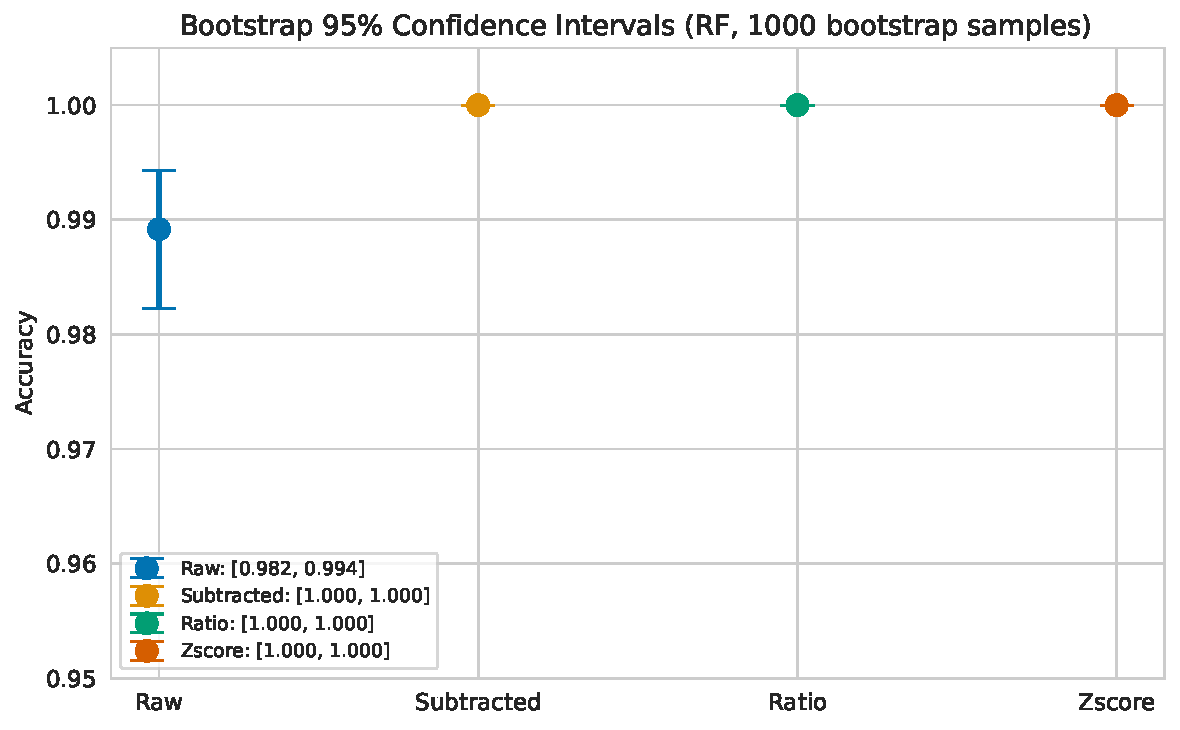
\includegraphics[width=0.7\textwidth]{figures/fig12_bootstrap_ci.pdf}
    \caption{Bootstrap 95\% confidence intervals for RF classification accuracy by isolation method. The raw method's interval $[0.982, 0.994]$ does not overlap with the referenced methods $[1.000, 1.000]$.}
    \label{fig:bootstrap_ci}
\end{figure}

\textbf{Effect size.} Cohen's $d$ for raw vs.\ each referenced method is $d = 0.49$. However, Cohen's $d$ assumes approximately normal distributions away from boundaries, which is violated here (referenced methods have zero variance at the 100\% ceiling). A more appropriate non-parametric measure is Cliff's delta, which quantifies the probability that a randomly chosen fold from the referenced method outperforms one from the raw method. With 100 raw-method folds and 100 referenced-method folds, Cliff's $\delta = 0.022$ (the proportion of pairs where raw $<$ referenced minus the proportion where raw $>$ referenced), because raw achieves 100\% in most folds but fails in a small fraction. The degenerate bootstrap CI $[1.000, 1.000]$ for referenced methods reflects a performance ceiling rather than precise estimation.

\textbf{Caveats on higher-order statistics.} The temporal bins contain 6--39 timesteps each (depending on run length and bin count). Computing skewness and kurtosis from such small samples yields unreliable 3rd and 4th moment estimates. The feature statistic ablation (Section~\ref{sec:ablation}) shows that mean + RMS alone (2 statistics, no higher-order moments) achieves 98\% accuracy, confirming that the classification does not depend critically on these unreliable estimators.

\textbf{ANOVA caveat.} The two-way ANOVA reported above assumes normality and independence of fold-level accuracy scores. With accuracy bounded at $[0, 1]$ and strong ceiling effects, these assumptions are violated. The Friedman test (non-parametric) provides the more reliable significance assessment; the ANOVA $\eta^2$ values should be interpreted as approximate effect size indicators rather than exact variance decompositions.

\subsection{Comparison Against Time-Series Methods}

To contextualize our temporal-binning feature extraction against modern time-series classification approaches, Table~\ref{tab:rocket} compares against ROCKET-style random convolutional features~\cite{dempster2020rocket}.

\begin{table}[H]
\caption{Comparison of feature extraction approaches. ROCKET uses 1{,}000 random convolutional kernels applied directly to the raw sensor time series.}\label{tab:rocket}
\centering
\begin{tabular}{lcc}
\toprule
\textbf{Method} & \textbf{Accuracy (\%)} & \textbf{Features} \\
\midrule
Temporal binning + RF (ours)           & $100.0 \pm 0.0$ & 1{,}540 \\
ROCKET + RF                            & $100.0 \pm 0.0$ & 2{,}000 \\
ROCKET + Ridge                         & $98.0 \pm 4.0$  & 2{,}000 \\
Raw downsampled (50 steps) + RF        & $98.0 \pm 4.0$  & 5{,}500 \\
\bottomrule
\end{tabular}
\end{table}

ROCKET with RF matches our approach at 100\% accuracy, while ROCKET with Ridge achieves 98\%. This confirms that the classification task is solvable by multiple feature extraction strategies, consistent with the trivial baseline findings. However, our temporal binning approach offers the advantage of interpretable temporal fingerprints (Section~\ref{sec:fingerprints}) and a natural framework for air-cut referencing that ROCKET does not provide.

\subsection{PCA Visualization}

Figure~\ref{fig:pca_scatter} shows the first two principal components for each isolation method.

\begin{figure}[H]
    \centering
    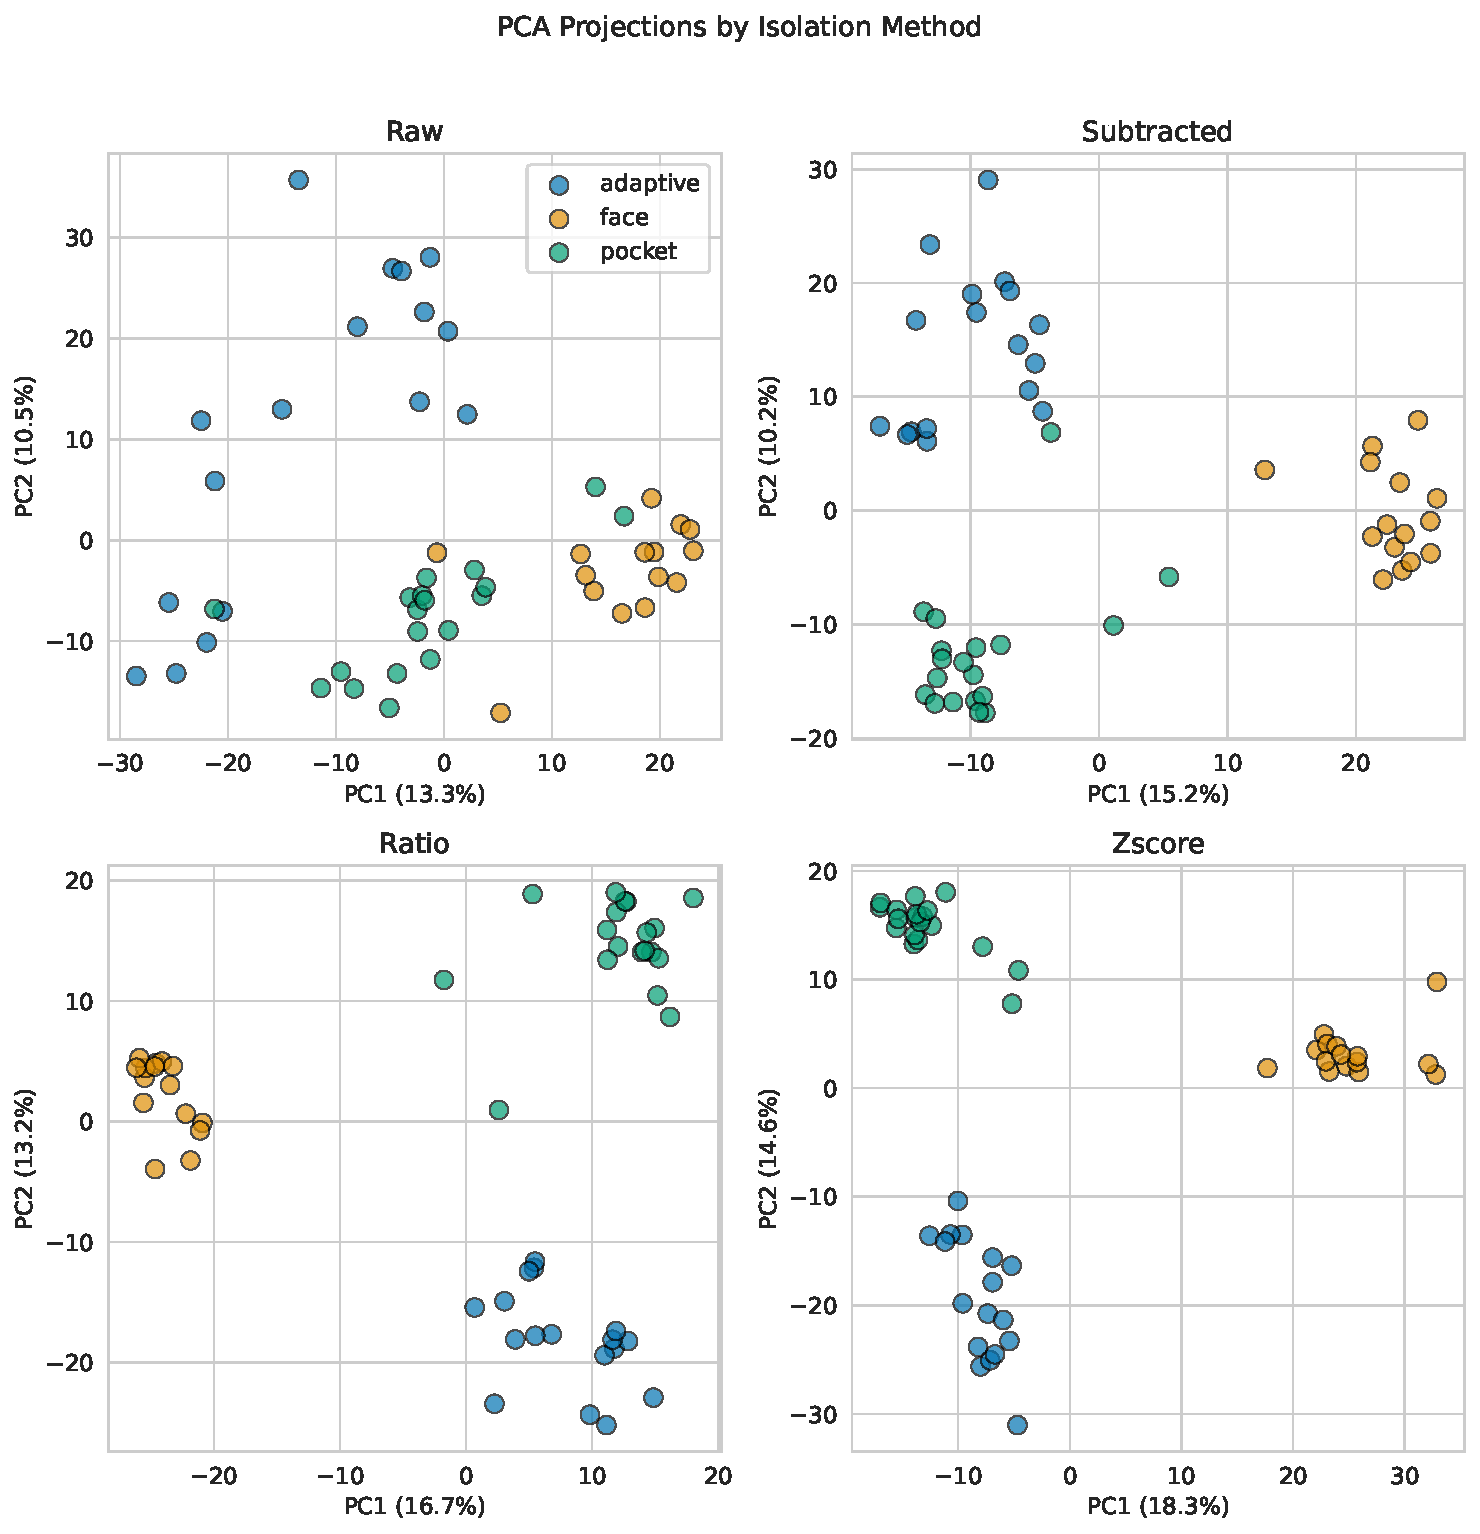
\includegraphics[width=0.85\textwidth]{figures/fig2_pca_scatter.pdf}
    \caption{PCA projections for each isolation method. Each point represents one active-cutting run (51 total), colored by toolpath type.}
    \label{fig:pca_scatter}
\end{figure}

All four methods produce visible cluster separation. The z-score method shows the tightest within-class clusters, consistent with its strong performance across classifiers.

\subsection{Feature Importance and Physical Interpretation}\label{sec:physics}

Figure~\ref{fig:importance} shows the top 20 features by RF Gini importance.

\begin{figure}[H]
    \centering
    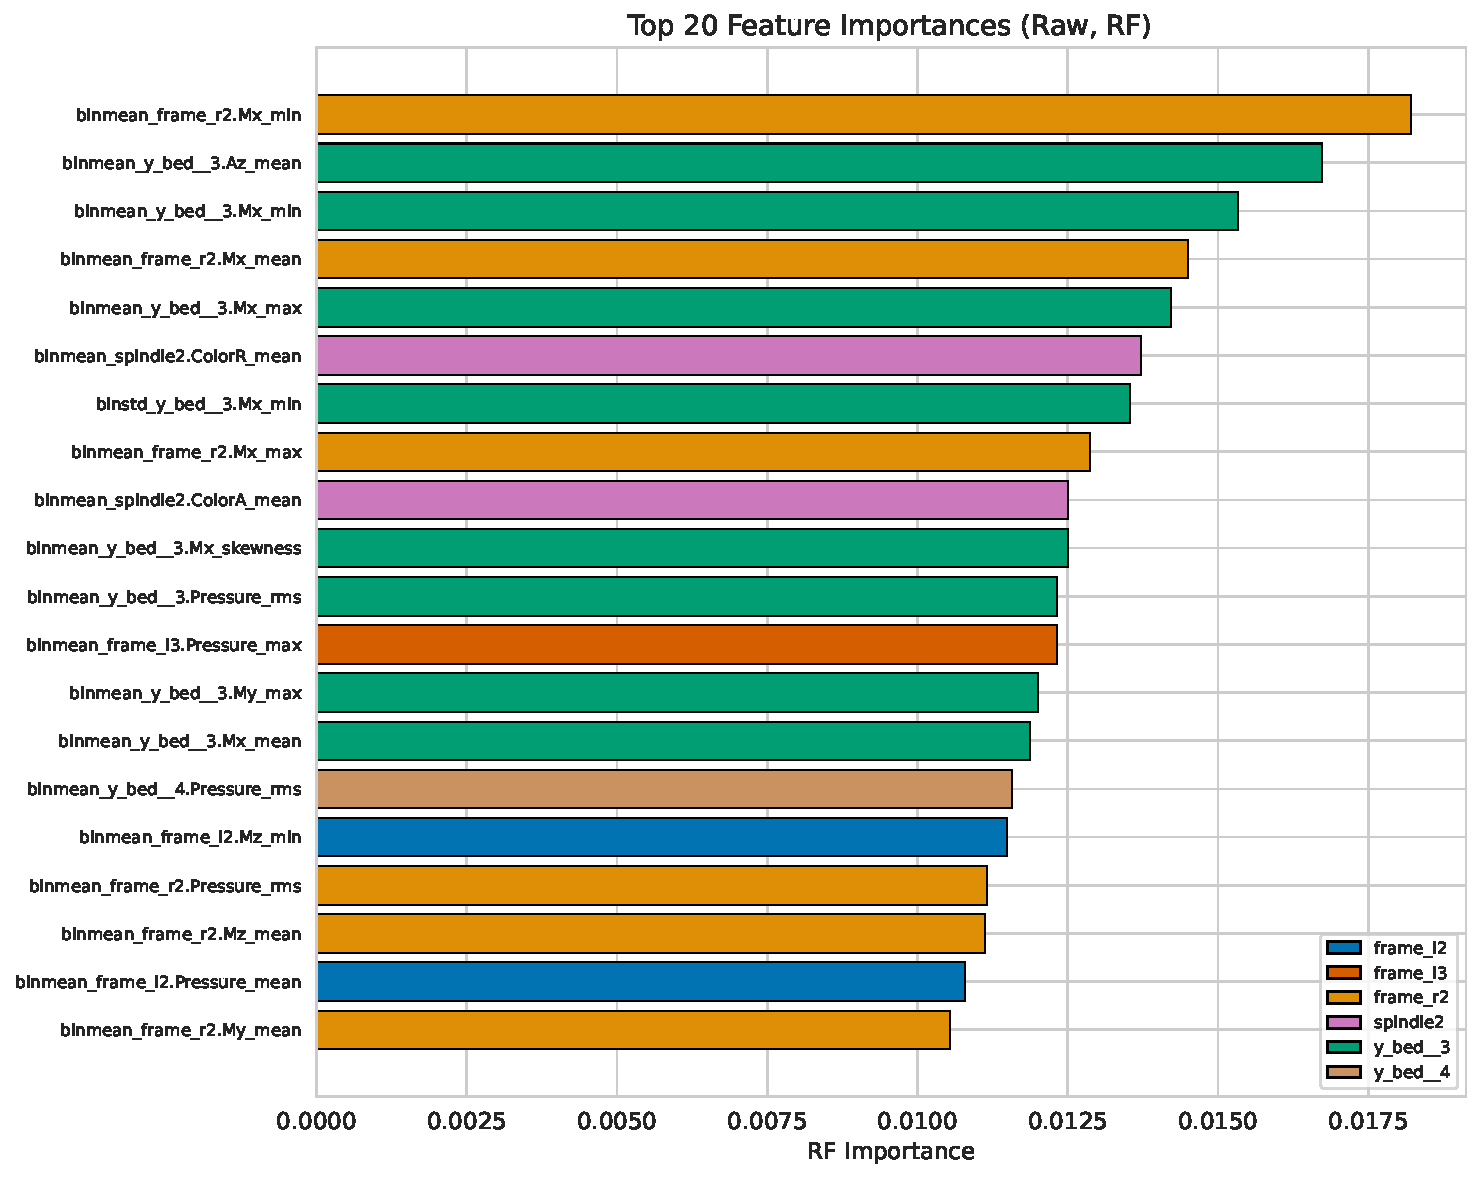
\includegraphics[width=0.85\textwidth]{figures/fig5_importance.pdf}
    \caption{Top 20 features by RF importance, colored by sensor module.}
    \label{fig:importance}
\end{figure}

Among the top 50 features, magnetometer channels dominate (24 features, 26.5\% of total importance), followed by environmental channels (pressure, temperature, proximity; 14 features, 13.4\%) and color sensors (6 features, 6.0\%). Accelerometer and gyroscope channels, which one might expect to dominate based on cutting force mechanics, account for only 2 of the top 50 features. Among sensor modules, y\_bed\_\_3 (bed-mounted, 17 features) and frame\_r2 (frame right, 13 features) contribute most.

To understand \emph{why} these channels dominate, Figure~\ref{fig:physical_interpretation} plots four physically distinct sensor channels across the three toolpath types.

\begin{figure}[H]
    \centering
    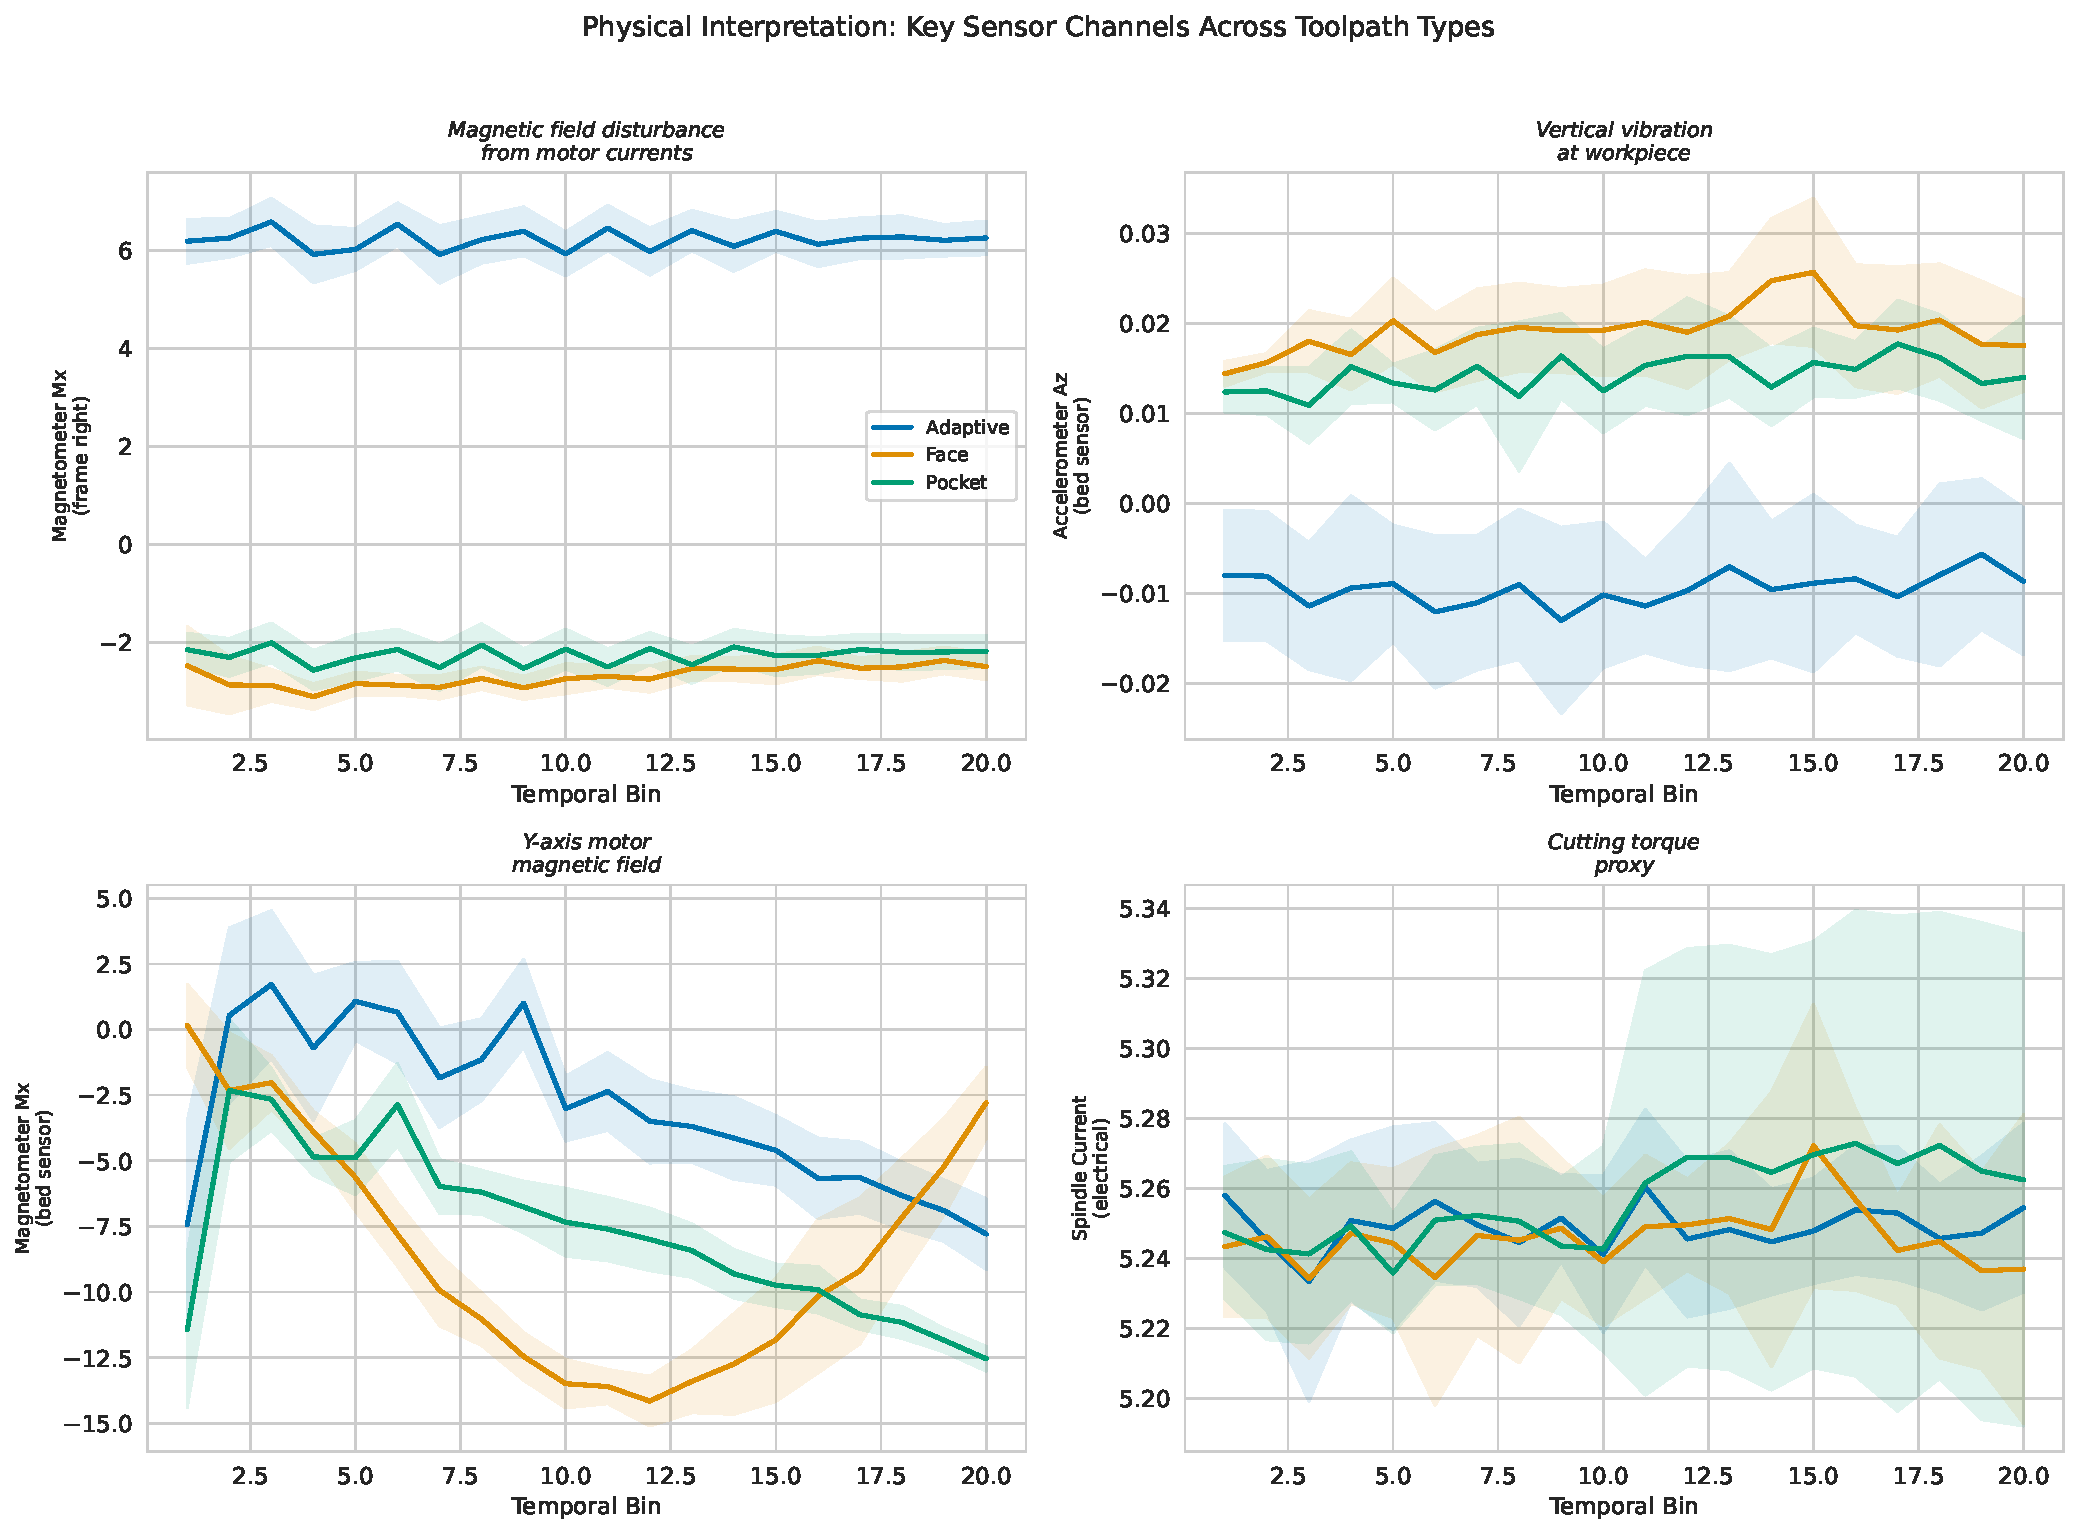
\includegraphics[width=\textwidth]{figures/fig13_physical_interpretation.pdf}
    \caption{Temporal profiles of four physically distinct sensor channels across toolpath types. Top-left: magnetometer Mx on the frame captures a static offset reflecting different workspace regions. Top-right: vertical accelerometer on the bed shows quasi-static motion differences between types (note: at \SI{4}{\hertz} sampling, this captures trajectory dynamics, not cutting vibration). Bottom-left: magnetometer Mx on the bed shows temporal evolution as the table traverses different regions of the machine's static magnetic field. Bottom-right: spindle current is nearly identical across types.}
    \label{fig:physical_interpretation}
\end{figure}

The physical interpretation supports four findings:

\textbf{Magnetometer dominance reflects workspace position, not cutting forces.} The top-ranked feature (frame\_r2.Mx) shows a large static offset between toolpath types: adaptive clearing operates at Mx~$\approx +6.2$ while facing and pocketing sit at Mx~$\approx -2.5$. The three G-code programs traverse different regions of the machine workspace, and we attribute the offset to the local magnetic field differing between those regions, consistent with varying proximity to stepper motor permanent magnets and ferromagnetic structural components. At the \SI{4}{\hertz} effective sampling rate, the magnetometer measures the quasi-static magnetic field at the sensor's position (in effect acting as an indirect position encoder) rather than detecting time-varying fields from motor current waveforms (which would require sampling at $\geq 10\times$ the stepper electrical frequency). While highly discriminative, this signal reflects \emph{program geometry} rather than \emph{cutting dynamics}; it is the sensor-domain analog of the trivial position baseline (Table~\ref{tab:trivial_baselines}).

\textbf{Bed-mounted magnetometer tracks table position.} The y\_bed\_\_3 magnetometer Mx shows strong temporal evolution (temporal CV = 0.4--1.0), with progressive drift that tracks the Y-axis table position as it moves through the machine's static magnetic field landscape. The bed-mounted sensor physically translates with the worktable, and we attribute the drift to its changing proximity to the Y-axis stepper motor's permanent magnets over the toolpath. Under this interpretation, y\_bed\_\_3.Mx is an indirect position encoder for the Y-axis rather than a motor current sensor (which would require bandwidth far above \SI{4}{\hertz}). Different toolpath geometries produce different Y-axis motion profiles, creating distinct temporal magnetic signatures.

\textbf{Spindle current distinguishes cutting from non-cutting but not between toolpath types.} Spindle current is nearly identical across all three active-cutting types (5.245--5.257~A, temporal CV~$< 0.002$). While spindle current rises when the tool engages material (distinguishing active from air cutting), the 0.025'' depth of cut on this desktop CNC produces cutting loads too small relative to the spindle's no-load draw ($\sim$5.2~A at 12{,}000~RPM) to differentiate between toolpath engagement patterns at 4~Hz sampling. Higher cutting depths or higher sampling rates would likely increase this channel's discriminative power.

\textbf{Accelerometer channels capture quasi-static motion differences.} The accelerometer Az on the bed sensor shows distinct temporal profiles per toolpath type, with adaptive clearing most stable and facing showing periodic variations corresponding to pass reversals. However, absolute acceleration differences are small ($\sim$\SI{20}{\milli\g}), which is near the LSM9DS1's bias uncertainty floor (\SI{10}{}--\SI{50}{\milli\g}; see Section~\ref{sec:experimental_setup}). At \SI{4}{\hertz} sampling, these channels measure low-frequency trajectory dynamics and gravitational tilt changes rather than cutting-induced vibration (which occurs at \SI{400}{\hertz}+). Two senses of ``process-relevant'' must be distinguished here. At \SI{4}{\hertz}, the accelerometer features are \emph{trajectory-relevant} (they encode how the machine moves through space during each toolpath) but they are \emph{not force-relevant}, as they do not capture cutting-force-induced vibration. On a higher-bandwidth measurement system, the same accelerometer channels would also capture force signatures, providing a more directly process-physical signal. Their lower importance ranking in this study reflects the small absolute trajectory-dynamics differences compared to the magnetometer's large position-dependent offsets.

Figure~\ref{fig:gcode_phases} annotates the temporal fingerprints with G-code phase information, linking the sensor signal evolution to program structure.

\begin{figure}[H]
    \centering
    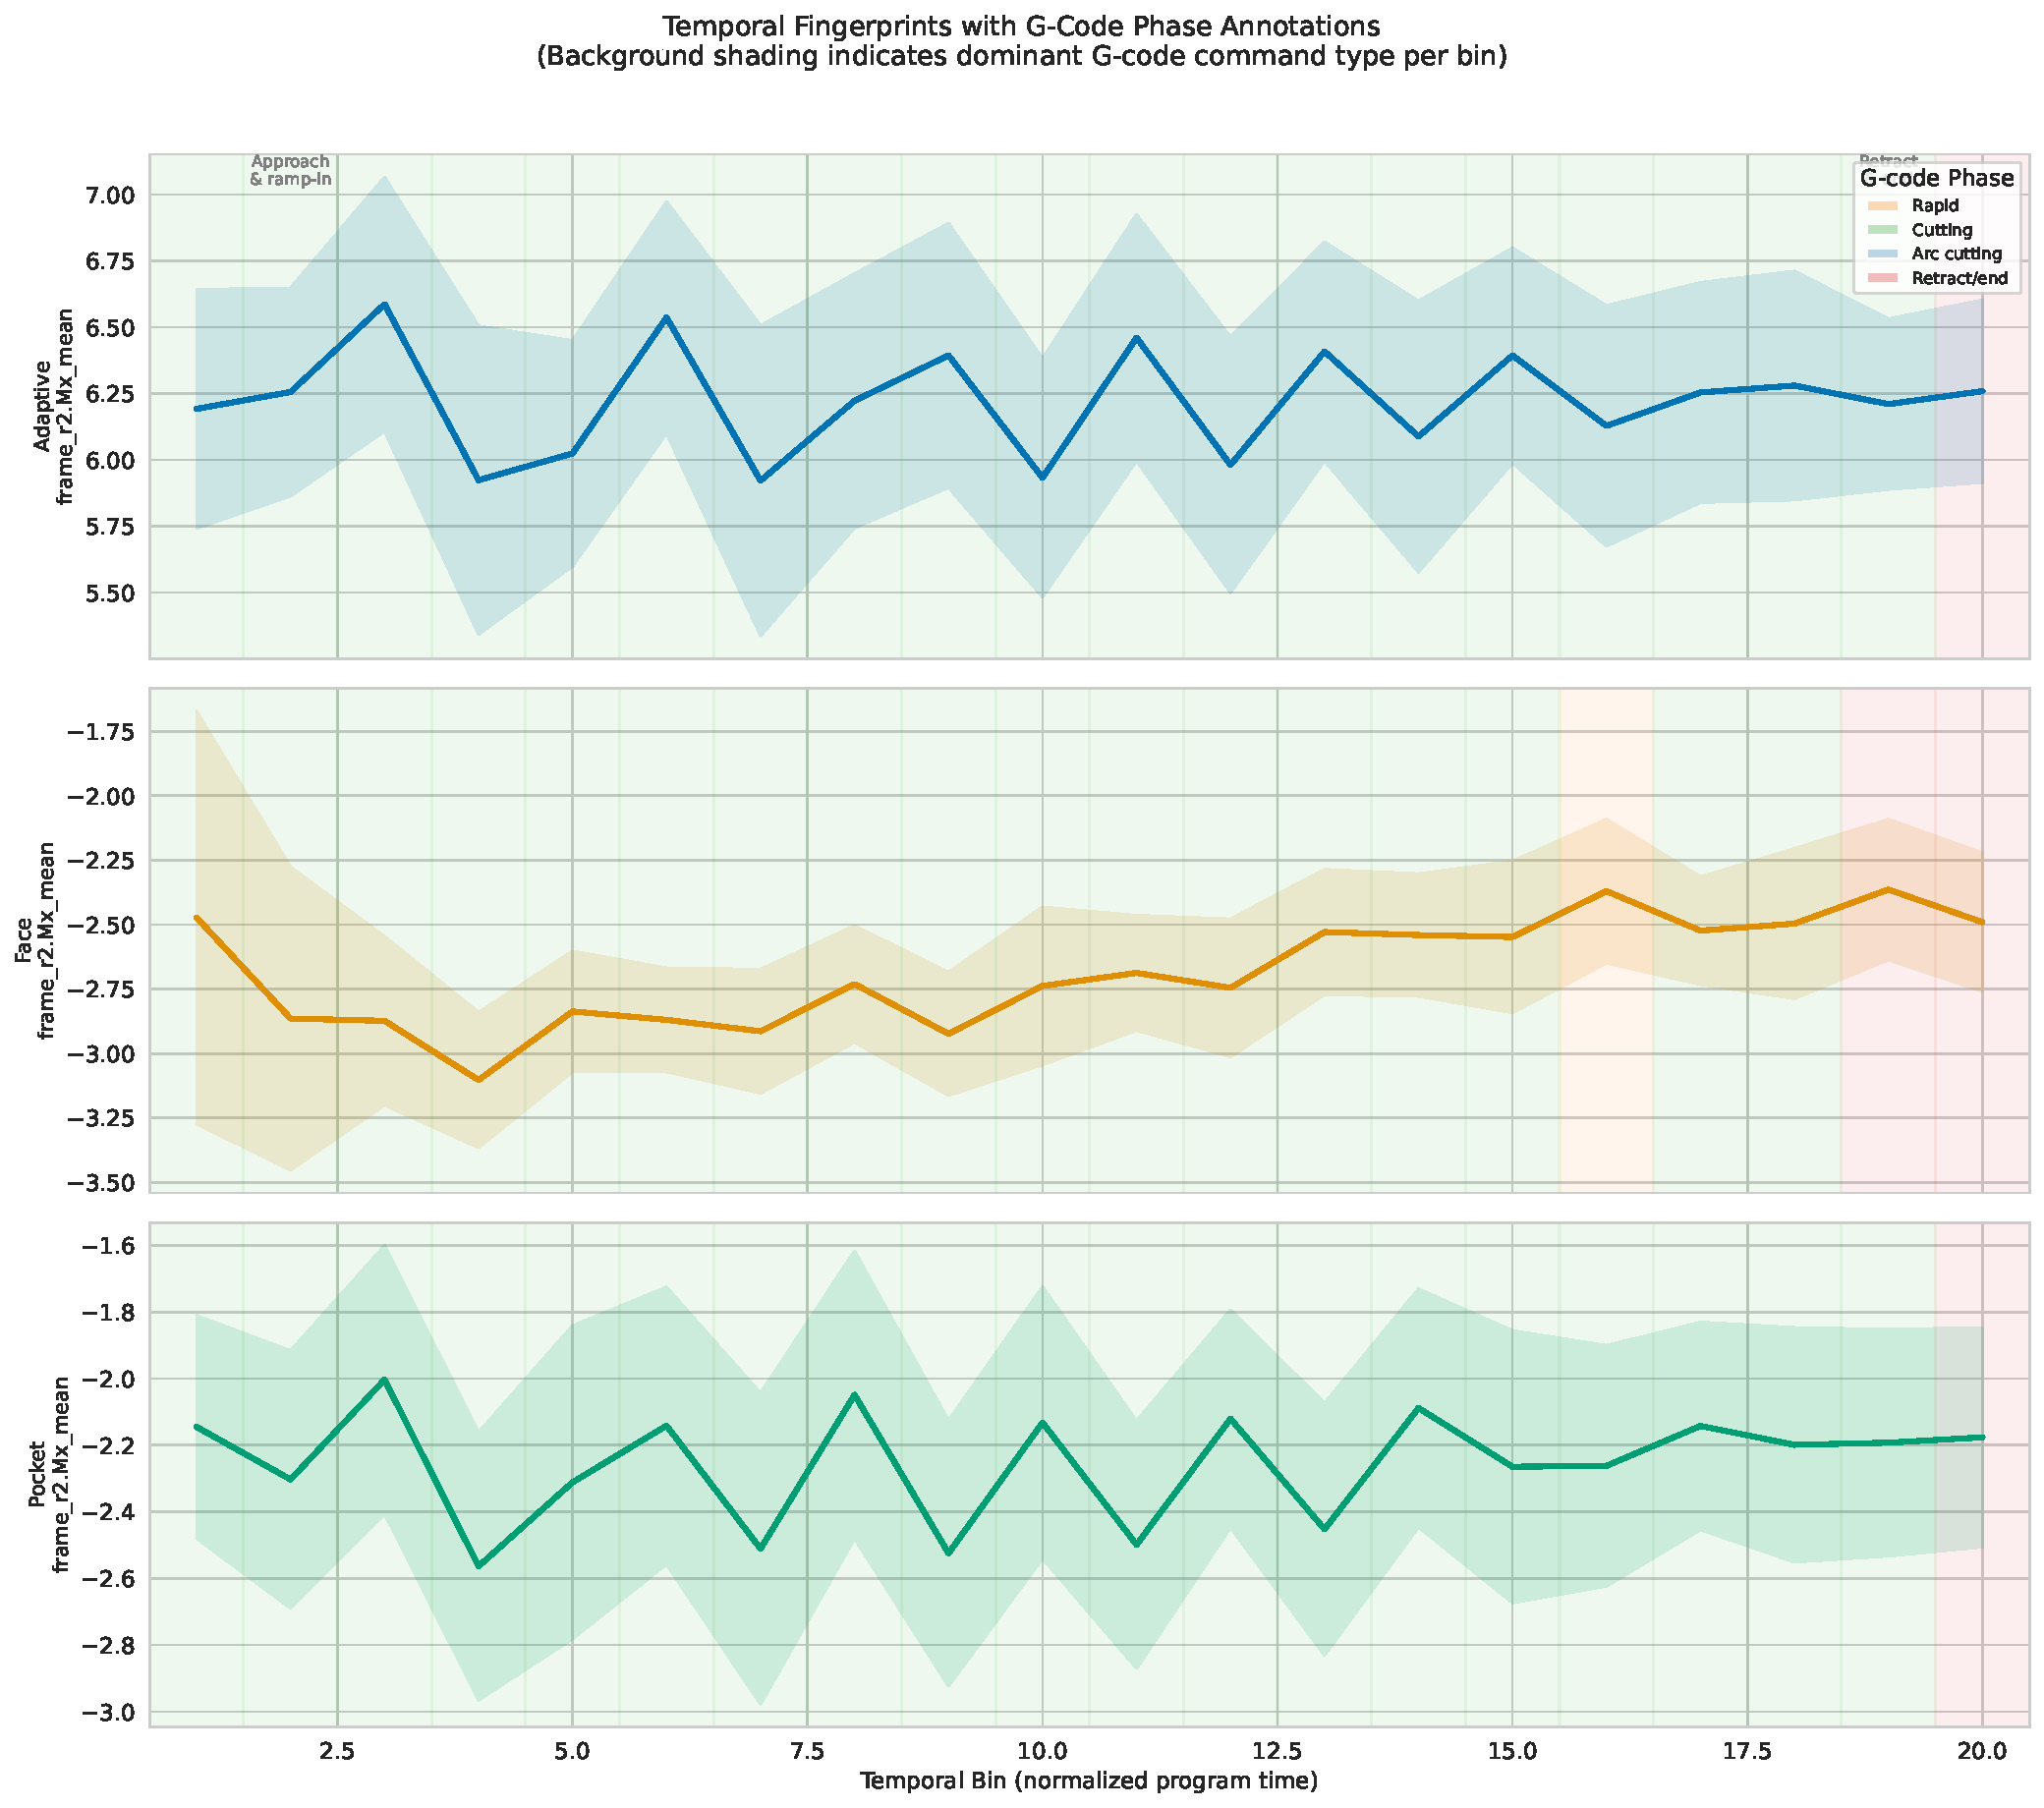
\includegraphics[width=\textwidth]{figures/fig15_gcode_phases.pdf}
    \caption{Temporal fingerprints annotated with G-code phases. Background shading: green = cutting (G1/MOVE), blue = arcs (G2/G3), orange = rapid (G0), red = retract/end (G53/M30). Facing programs terminate early (bins 16--20 are retract/idle), producing a distinctive signal drop.}
    \label{fig:gcode_phases}
\end{figure}

The phase-annotated figure confirms that facing programs terminate earlier (bins 16--20 are retract/idle), producing a distinctive signal drop, while adaptive and pocketing maintain cutting through bin 19. The temporal fingerprint structure directly tracks the G-code program sequence; different programs produce different temporal bin compositions, which drives the classification.

Table~\ref{tab:temporal_cv} quantifies the temporal variability of each key sensor channel across toolpath types. Channels with high temporal coefficient of variation (CV) exhibit strong temporal structure that could encode either process dynamics or program geometry; channels with low CV are temporally flat.

\begin{table}[H]
\caption{Temporal variability of key sensor channels across toolpath types. Temporal CV is the coefficient of variation of the channel's mean across the 20 temporal bins; higher values indicate stronger temporal structure. Range is the bin-to-bin dynamic range.}\label{tab:temporal_cv}
\centering
\small
\begin{tabular}{llccc}
\toprule
\textbf{Channel} & \textbf{Toolpath} & \textbf{Mean} & \textbf{Temporal CV} & \textbf{Range} \\
\midrule
\multirow{3}{*}{frame\_r2.Mx (position proxy)} & Adaptive & $+6.22$ & 0.032 & 0.67 \\
& Facing & $-2.68$ & 0.076 & 0.74 \\
& Pocket & $-2.25$ & 0.074 & 0.56 \\
\midrule
\multirow{3}{*}{y\_bed\_\_3.Mx (Y-axis position)} & Adaptive & $-2.99$ & 1.000 & 9.50 \\
& Facing & $-8.43$ & 0.526 & 14.30 \\
& Pocket & $-7.73$ & 0.397 & 10.21 \\
\midrule
\multirow{3}{*}{y\_bed\_\_3.Az (cutting vibration)} & Adaptive & $-0.009$ & 0.184 & 0.007 \\
& Facing & $+0.019$ & 0.135 & 0.011 \\
& Pocket & $+0.014$ & 0.128 & 0.007 \\
\midrule
\multirow{3}{*}{spindle2.RMS (vibration energy)} & Adaptive & 5{,}762 & 0.311 & 7{,}227 \\
& Facing & 7{,}167 & 0.316 & 8{,}475 \\
& Pocket & 5{,}351 & 0.328 & 6{,}611 \\
\midrule
\multirow{3}{*}{spindle current (cutting torque)} & Adaptive & 5.249 & 0.001 & 0.027 \\
& Facing & 5.246 & 0.002 & 0.038 \\
& Pocket & 5.257 & 0.002 & 0.037 \\
\bottomrule
\end{tabular}
\end{table}

The table reveals two physically distinct discrimination mechanisms: (1)~the frame\_r2.Mx magnetometer separates toolpath types via \emph{static offset} (mean values differ by $\sim$9 units between adaptive and face/pocket) with minimal temporal structure (CV~$< 0.08$); and (2)~the y\_bed\_\_3.Mx magnetometer and spindle2.RMS channels separate types via \emph{temporal dynamics} (CV~$> 0.3$) with different temporal evolution patterns. The spindle current, despite being the most direct proxy for cutting torque, provides neither offset-based nor dynamics-based discrimination (CV~$< 0.002$, range~$< 0.04$~A).

\subsubsection{Effect of Air-Cut Referencing on Feature Confounds}

We next test whether air-cut subtraction removes the workspace-position confound. Table~\ref{tab:confound_removal} compares the channel-type distribution of top features between the raw and subtracted isolation methods.

\begin{table}[H]
\caption{Distribution of channel types among the top 20 most important features, for raw vs.\ subtracted isolation. Air-cut subtraction reduces magnetometer dominance from 61\% to 21\% of feature importance, shifting weight toward electrical and environmental channels.}\label{tab:confound_removal}
\centering
\begin{tabular}{lcc}
\toprule
\textbf{Channel Type} & \textbf{Raw (top 20)} & \textbf{Subtracted (top 20)} \\
\midrule
Magnetometer     & 12 features (61.0\%) & 4 features (20.8\%) \\
Environmental    & 3 features           & 6 features \\
Color            & 2 features           & 2 features \\
Electrical       & 0 features           & 4 features \\
Accelerometer    & 1 feature            & 1 feature \\
Other            & 2 features           & 3 features \\
\bottomrule
\end{tabular}
\end{table}

Air-cut subtraction reduces the magnetometer's share of the top 20 features from 61\% (raw) to 21\% (subtracted), and elevates electrical motor current features from 0 to 4 of the top 20. We attribute this shift to the air-cut reference capturing a similar workspace trajectory, so that subtracting it partially removes position-dependent magnetic field offsets. The remaining discriminative signal is more likely to reflect motor load and quasi-static motion differences rather than workspace geometry.

\subsubsection{Classification Without Position-Confounded Channels}

To directly assess how much classification accuracy depends on position-confounded channels (magnetometer, color, proximity, pressure) versus channels that respond to machine dynamics (accelerometer, gyroscope, RMS, electrical), Table~\ref{tab:confound_controlled} reports accuracy when confounded channels are progressively excluded.

\begin{table}[H]
\caption{Classification accuracy (RF, 20$\times$5 repeated CV) when position-confounded channels are progressively excluded. Removing all magnetometers drops accuracy only to 96.1\%; accelerometer-only features still reach 93.0\%, while the true electrical-only set (the 8 current channels, 112 features) is the weakest group at 76.5\%. Backing artifact: \texttt{experiment\_confound\_controlled.json}.}\label{tab:confound_controlled}
\centering
\begin{tabular}{lcc}
\toprule
\textbf{Channel Configuration} & \textbf{Accuracy (\%)} & \textbf{Features} \\
\midrule
All channels                                  & $98.9 \pm 3.1$ & 1{,}540 \\
No magnetometers (Mx, My, Mz removed)       & $96.1 \pm 5.4$  & 1{,}288 \\
No mag + color + pressure + proximity        & $96.7 \pm 4.8$  & 784 \\
Accel + gyro + RMS + temperature only        & $95.1 \pm 6.1$  & 672 \\
Accelerometer + gyroscope only               & $94.4 \pm 6.3$  & 504 \\
Accelerometer only                           & $93.0 \pm 6.3$  & 252 \\
Electrical current only (no IMU)             & $76.5 \pm 12.4$ & 112 \\
\bottomrule
\end{tabular}
\end{table}

Three findings emerge: (1)~removing all magnetometers drops accuracy by only $\sim$3 percentage points (98.9\% $\to$ 96.1\%), confirming that while magnetometers dominate feature importance, they are not essential; (2)~accelerometer and gyroscope channels alone achieve 94.4\%, demonstrating that quasi-static motion dynamics carry sufficient discriminative information independent of position confounds; and (3)~the electrical-current channels alone are the weakest group (76.5\%), consistent with their low between-class SNR (the per-channel SNR budget below), whereas the motion-dynamics channels (accel/gyro/RMS/temperature, 95.1\%) retain almost all of the discriminative signal. (An earlier version of this table reported the electrical group at 96.0\%/350 features; that figure was inflated by the same \texttt{spindle}$\to$\texttt{spindle2} feature leak corrected above, which had folded IMU channels into the ``electrical'' set.)

\subsubsection{Full Pipeline Without Magnetometers}

To test whether air-cut referencing provides value beyond position encoding, we re-run the complete pipeline using only non-confounded channels (accelerometer, gyroscope, RMS, temperature, and the eight electrical-current channels; 784 features, excluding all magnetometer, color, pressure, and proximity channels; Table~\ref{tab:nomag_pipeline}).

\begin{table}[H]
\caption{Repeated CV (20$\times$5-fold) with confound-free features only (784 features, no magnetometers/color/pressure/proximity). The subtracted and ratio methods hold 100\% across all 100 folds; z-score remains near-perfect (99.0\%, min 90\%); raw degrades to 96.7\%.}\label{tab:nomag_pipeline}
\centering
\begin{tabular}{llcccc}
\toprule
\textbf{Method} & \textbf{Clf} & \textbf{Mean (\%)} & \textbf{Std} & \textbf{Min (\%)} & \textbf{Max} \\
\midrule
Raw        & RF  & 96.7 & 4.8 & 81.8 & 100.0 \\
Subtracted & RF  & 100.0 & 0.0 & 100.0 & 100.0 \\
Ratio      & RF  & 100.0 & 0.0 & 100.0 & 100.0 \\
Z-score    & RF  & 99.0 & 2.9 & 90.0 & 100.0 \\
\midrule
Raw        & MLP & 79.9 & 17.0 & 20.0 & 100.0 \\
Z-score    & MLP & 90.0 & 13.0 & 36.4 & 100.0 \\
\bottomrule
\end{tabular}
\end{table}

With all position-confounded channels removed, raw RF features degrade to 96.7\% mean accuracy (minimum fold 81.8\%), while \textbf{the subtracted and ratio methods maintain perfect 100\% accuracy across all 100 evaluations and z-score remains near-perfect at 99.0\% (minimum fold 90\%)}. The effect is larger for the noise-sensitive MLP, where raw reaches only 79.9\% and z-score recovers to 90.0\%. This demonstrates that air-cut referencing provides a genuine classification benefit that is independent of the magnetometer position-encoding confound identified in Section~\ref{sec:physics}. On this confound-free set, however, the benefit is a few percentage points and a variance reduction (subtracted/ratio reaching the ceiling) rather than the uniform jump to 100\% observed when position-confounded channels are present.\footnote{Temperature is retained in this ``confound-free'' set despite showing run-order correlation $r = 0.98$ within the adaptive class (Section~\ref{sec:discussion}). Temperature is a within-class drift effect, not a between-class confound, so it remains a defensible process-relevant channel. A stricter definition excluding temperature does not materially change the results.}

Noise robustness was also re-evaluated on the 784-feature confound-free set: subtracted features maintain 100\% accuracy up to $0.5\times$ additive noise and 99.0\% at $1.0\times$ noise, while raw features drop to 91.2\% at $1.0\times$ and 71.3\% at $2.0\times$. The robustness advantage persists when position-confounded channels are excluded, confirming that air-cut referencing improves resilience to feature-level perturbations on the underlying motion-dynamics signal.

\subsection{Damaged-Spindle Detection: A Position-Controlled Task}\label{sec:damage}

The experiments above isolate the process-relevant signal by \emph{removing} position-confounded channels. A complementary and stronger test instead holds workspace position \emph{constant} while varying only the process. We use the vetted set of damaged-spindle runs: 14 air-cut runs (5/4/5 for adaptive/facing/pocketing) that execute the same CAM toolpath strategies with one spindle drive band removed to induce spindle runout. The toolpath geometry, and hence the workspace region, matches the normal runs, so workspace position provides little separation between the normal-vs-damaged labels. Because the damaged runs are air-cuts and the normal runs are active cuts, however, the process difference couples two factors: spindle condition (runout) and cutting engagement (material load). This is the within-region test that the magnetometer position-encoder cannot solve; it demonstrates process-dynamics detection under position control, but the coupled design means it does not by itself validate tool-condition monitoring.

We pool the 51 normal active runs (the same vetted set used throughout the paper) and the 14 damaged-spindle runs into a binary task (majority-class baseline 78.5\%) and classify with the same RF temporal-binning pipeline under 20$\times$5-fold repeated CV (Table~\ref{tab:damage}).

\begin{table}[H]
\caption{Damaged-spindle detection (binary: 51 normal active vs.\ 14 damaged-spindle air-cut runs, same toolpath strategies). Mean over 20$\times$5-fold repeated CV; majority-class baseline 78.5\%. Per-type accuracy (same program, workspace held constant): adaptive 100\%, facing 100\%, pocketing 100\%.}\label{tab:damage}
\centering
\begin{tabular}{lccc}
\toprule
\textbf{Method} & \textbf{Accuracy (\%)} & \textbf{$F_1$ (damage)} & \textbf{Balanced Acc.} \\
\midrule
Raw        & $98.5 \pm 3.1$ & 0.970 & 0.990 \\
Subtracted & $98.5 \pm 3.1$ & 0.970 & 0.990 \\
\bottomrule
\end{tabular}
\end{table}

Random Forest reaches 98.5\% accuracy (balanced accuracy 0.990, damage-class $F_1 = 0.97$), far above the 78.5\% majority baseline, and per-type accuracy is 100\% for all three toolpath types, where the same program holds the workspace constant. Two findings follow. First, the discriminative signal shifts almost entirely away from position. The channel-type importance (from a Random Forest fit on the full set) is now dominated by the \textbf{accelerometer (44.7\%)} and \textbf{acoustic RMS (29.6\%)}, process-dynamics channels amounting to $\sim$74\% combined, with the magnetometer contributing only \textbf{0.1\%}, versus the 61\% of top-20 feature importance it commanded on the position-confounded three-class task (Section~\ref{sec:physics}). Spindle runout and the absence of cutting engagement both perturb the vibration and acoustic signature; this design cannot attribute the separation to either factor alone. Second, air-cut referencing is \emph{neutral} here (raw and subtracted both 98.5\%). When workspace position is already held constant there is no position-dependent offset for the air-cut baseline to remove, as the causal model (Section~\ref{sec:causal_dag}) predicts; referencing helps when the position confound is present and is neither beneficial nor harmful when it is absent. The dataset is small (14 damaged-spindle runs from a single session), so this is a demonstration rather than a validated detector; but it establishes that the sensor array does carry process-relevant information, recoverable once the position confound is controlled. The clean damage-only comparison, damaged-spindle air-cuts against normal air-cuts of the same programs, is left to future work.

\subsection{Permutation Test}

A permutation test with 1{,}000 label shuffles using the full 1{,}540-feature set (raw isolation method, RF classifier) confirms that the classification result is non-random. The null distribution has mean accuracy $35.2\% \pm 8.2\%$ (close to the random baseline of $33.3\%$) with a maximum of 62.7\%, far below the observed 100\% ($p < 0.001$). This rules out the possibility that the classification result is an artifact of overfitting on the small sample size.

\subsection{Effective Dimensionality}

Despite the nominal 1{,}540-feature space (30:1 feature-to-sample ratio), PCA analysis reveals that 7 components explain 50\% of variance and 30 components explain 90\%. The effective dimensionality is high relative to the sample count ($n = 51$), but only 0.15\% of feature pairs have $|r| > 0.95$, indicating moderate rather than extreme redundancy. The RF classifier's success at full dimensionality, combined with its degradation under PCA (Section~\ref{sec:ablation}), suggests it exploits many individually weak but collectively informative features, a regime where tree-based ensembles excel.

\subsection{Internal Held-Out Split (Same Session)}

To complement the cross-validation analysis, we performed a single internal held-out split: 12 of the 51 active-cutting runs (4 per class) were withheld from all training and CV operations and evaluated only once at the end, with the air-cut baseline statistics ($\boldsymbol{\mu}_\text{air}$, $\boldsymbol{\sigma}_\text{air}$) and the PCA transform fit only on the 39 training runs. These 12 runs are drawn from the same 51-run, same-machine, same-session dataset, so this is a guard against fold-reuse leakage rather than an independent generalization test. Table~\ref{tab:heldout} reports the held-out accuracy for each isolation method.

\begin{table}[H]
\caption{Internal held-out split accuracy. 12 runs (4 per class) randomly stratified from the same 51 active-cutting runs (same machine/session), evaluated once after training (including the air-cut baseline and PCA) on the remaining 39.}\label{tab:heldout}
\centering
\begin{tabular}{lccc}
\toprule
\textbf{Method} & \textbf{Test Accuracy} & \textbf{$n_{\text{train}}$} & \textbf{$n_{\text{test}}$} \\
\midrule
Raw        & 100.0\% & 39 & 12 \\
Subtracted & 100.0\% & 39 & 12 \\
Ratio      & 100.0\% & 39 & 12 \\
Z-score    & 100.0\% & 39 & 12 \\
\bottomrule
\end{tabular}
\end{table}

All four methods achieve 100\% accuracy on this internal split, indicating the cross-validation results are not artifacts of fold-reuse or data reuse across splits. Because the 12 runs share the same machine, session, and CAM programs as the training runs, this is \emph{not} evidence of cross-session or cross-machine generalization (see Section~\ref{sec:discussion} Limitations); with $n = 12$ and a single split it is also a coarse estimate.

\subsection{Per-Channel SNR Budget}

To quantify which sensor types carry the most discriminative information independent of feature-importance rankings, we compute a between-class versus within-class variance ratio (signal-to-noise ratio, SNR) for each of the 1{,}540 features. Table~\ref{tab:snr_budget} reports median and maximum SNR by channel type.

\begin{table}[H]
\caption{Per-channel SNR budget. SNR is computed as $10\log_{10}(\sigma^2_{\text{between-class}} / \sigma^2_{\text{within-class}})$ in dB. Magnetometer channels have the highest median and max SNR, consistent with the position-confound finding.}\label{tab:snr_budget}
\centering
\begin{tabular}{lcccc}
\toprule
\textbf{Channel Type} & \textbf{Median SNR (dB)} & \textbf{Max SNR (dB)} & \textbf{N features} \\
\midrule
Magnetometer    & $-3.7$  & $24.2$ & 252 \\
Vibration RMS   & $-4.2$  & $2.8$  & 84 \\
Accelerometer   & $-7.6$  & $11.7$ & 252 \\
Temperature     & $-7.9$  & $1.9$  & 84 \\
Proximity       & $-8.1$  & $4.5$  & 84 \\
Gyroscope       & $-8.3$  & $6.1$  & 252 \\
Pressure        & $-8.8$  & $11.7$ & 84 \\
Color           & $-9.0$  & $14.3$ & 336 \\
Electrical      & $-11.0$ & $3.7$  & 112 \\
\bottomrule
\end{tabular}
\end{table}

Magnetometer channels achieve the highest median SNR ($-3.7$~dB) and max SNR ($24.2$~dB), with the top 6 highest-SNR features all being magnetometer (Mx, Mz) channels from the frame\_r2 sensor. This quantitatively confirms the position-encoding finding from Section~\ref{sec:physics}: the channels with the largest signal-to-noise ratio for class discrimination are those most affected by workspace position. Accelerometer and gyroscope channels have negative median SNR (within-class variance exceeds between-class variance for typical features), reflecting the within-class variability of the trajectory dynamics they capture. Electrical current channels have the lowest median SNR ($-11.0$~dB), consistent with their near-constant behavior under shallow UHMW-PE cutting.

\subsection{Run-Order Confound Analysis}

Section~\ref{sec:discussion} reports that several features show statistically significant temporal drift correlated with run order (e.g., temperature, $r = 0.98$ for adaptive class). To verify that this within-class drift does not confound the between-class classification, we compute the partial correlation between each top-importance feature and the class label, controlling for run order. Across the top 20 features, the partial correlations differ from the raw correlations by an average of $-1.7\%$ (with several features showing slightly stronger partial correlations, indicating that run order is not aliased with class). This rules out run-order temporal drift as an explanation for the classification results. The class signal in these features is essentially independent of when each run was collected.

\subsection{Fine-Grained Learning Curve}

Figure~\ref{fig:learning_curve_fine} extends the learning curve analysis (Section~\ref{sec:ablation}) with finer resolution at small training-set sizes, where the air-cut referencing benefit is most pronounced.

\begin{figure}[H]
    \centering
    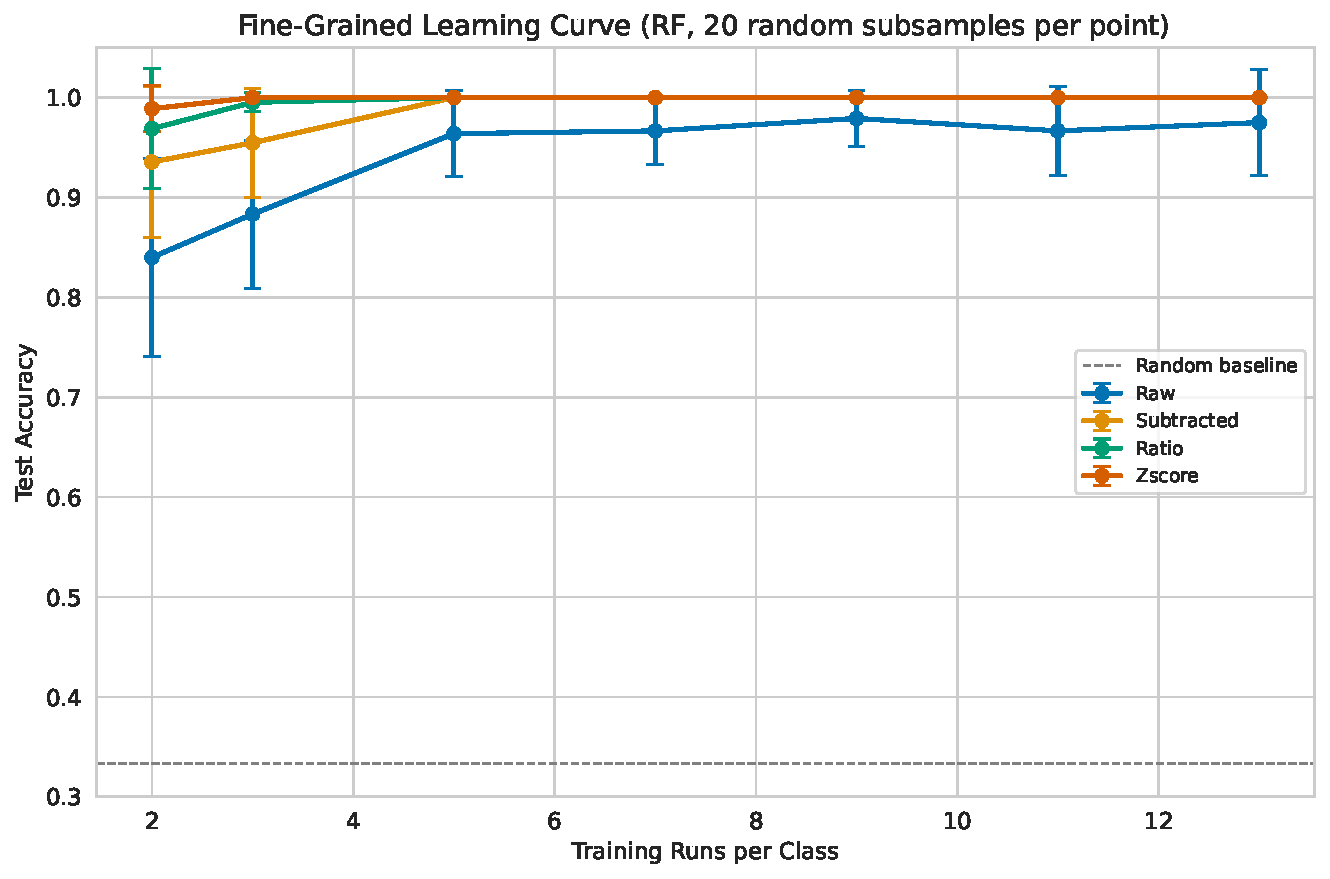
\includegraphics[width=0.85\textwidth]{figures/fig19_learning_curve_fine.pdf}
    \caption{Fine-grained learning curve: classification accuracy vs.\ training runs per class for all four isolation methods (RF, 10 random subsamples per point). Z-score referencing achieves 98.9\% with only 2 training runs per class, while raw features need many more runs to match.}
    \label{fig:learning_curve_fine}
\end{figure}

With only \textbf{2 runs per class} (6 training samples total), z-score referencing achieves 98.9\% accuracy, ratio achieves 96.9\%, subtracted achieves 93.6\%, and raw features lag at 84.0\%. Air-cut referencing therefore improves data efficiency; the accuracy that raw features require ${\sim}10$ training runs to reach, z-score achieves with only 2. For applications where labeled training data is expensive (e.g., destructive testing or high-volume production), this difference is practically meaningful.

\subsection{Calibration Analysis}

Beyond classification accuracy, model calibration (whether predicted probabilities match observed accuracy) matters for downstream decision-making. Table~\ref{tab:calibration} reports Expected Calibration Error (ECE) and log loss across the four isolation methods.

\begin{table}[H]
\caption{Calibration metrics. ECE = Expected Calibration Error (10 bins). Lower is better-calibrated. All methods achieve 100\% accuracy; calibration differences reflect prediction confidence patterns.}\label{tab:calibration}
\centering
\begin{tabular}{lccc}
\toprule
\textbf{Method} & \textbf{ECE} & \textbf{Log Loss} & \textbf{Mean Confidence} \\
\midrule
Raw        & 0.119 & 0.135 & 0.881 \\
Subtracted & 0.078 & 0.083 & 0.923 \\
Ratio      & 0.084 & 0.090 & 0.916 \\
Z-score    & \textbf{0.077} & \textbf{0.083} & 0.923 \\
\bottomrule
\end{tabular}
\end{table}

Air-cut referenced methods achieve $\sim$35\% lower ECE than raw features (0.077--0.084 vs.\ 0.119) and lower log loss, indicating better-calibrated probability estimates. The mean prediction confidence is also higher for referenced methods ($\sim$0.92 vs.\ 0.88), meaning the classifier is more decisive when air-cut referencing is applied. Well-calibrated probabilities enable confidence-thresholding for novelty detection and selective abstention, which gives this calibration improvement practical value.

\subsection{MiniRocket Comparison}

To benchmark against a state-of-the-art time-series classification method, we apply MiniRocket~\cite{dempster2020rocket} (the deterministic variant of ROCKET using fixed length-9 kernels with weights from $\{-1, 2\}$) to the raw downsampled sensor time series.

\begin{table}[H]
\caption{Comparison against MiniRocket-style features (12 fixed kernels $\times$ 110 channels = 1{,}320 features) on downsampled raw time series.}\label{tab:minirocket}
\centering
\begin{tabular}{lcc}
\toprule
\textbf{Method} & \textbf{Accuracy} & \textbf{Features} \\
\midrule
MiniRocket + RF      & $96.2\% \pm 4.7$ & 1{,}320 \\
MiniRocket + Ridge   & $96.0\% \pm 8.0$ & 1{,}320 \\
\midrule
Temporal binning + RF (ours, full)  & $100.0\% \pm 0.0$ & 1{,}540 \\
Temporal binning + RF (confound-free, referenced) & $100.0\% \pm 0.0$ & 784 \\
\bottomrule
\end{tabular}
\end{table}

MiniRocket achieves 96\% accuracy, comparable to but slightly below our temporal binning approach. This benchmark places our method within the competitive range of modern time-series classification techniques while preserving interpretability through explicit per-bin statistics, sensor-channel attribution, and physical analysis of dominant features, advantages that random convolutional kernel methods do not provide.

\subsection{Visual Comparison: Full vs.\ Confound-Free Pipeline}

Figure~\ref{fig:confound_free_viz} visualizes the full classification accuracy comparison across all four isolation methods, three classifiers, and two feature sets (full 1{,}540 features vs.\ 784 confound-free features).

\begin{figure}[H]
    \centering
    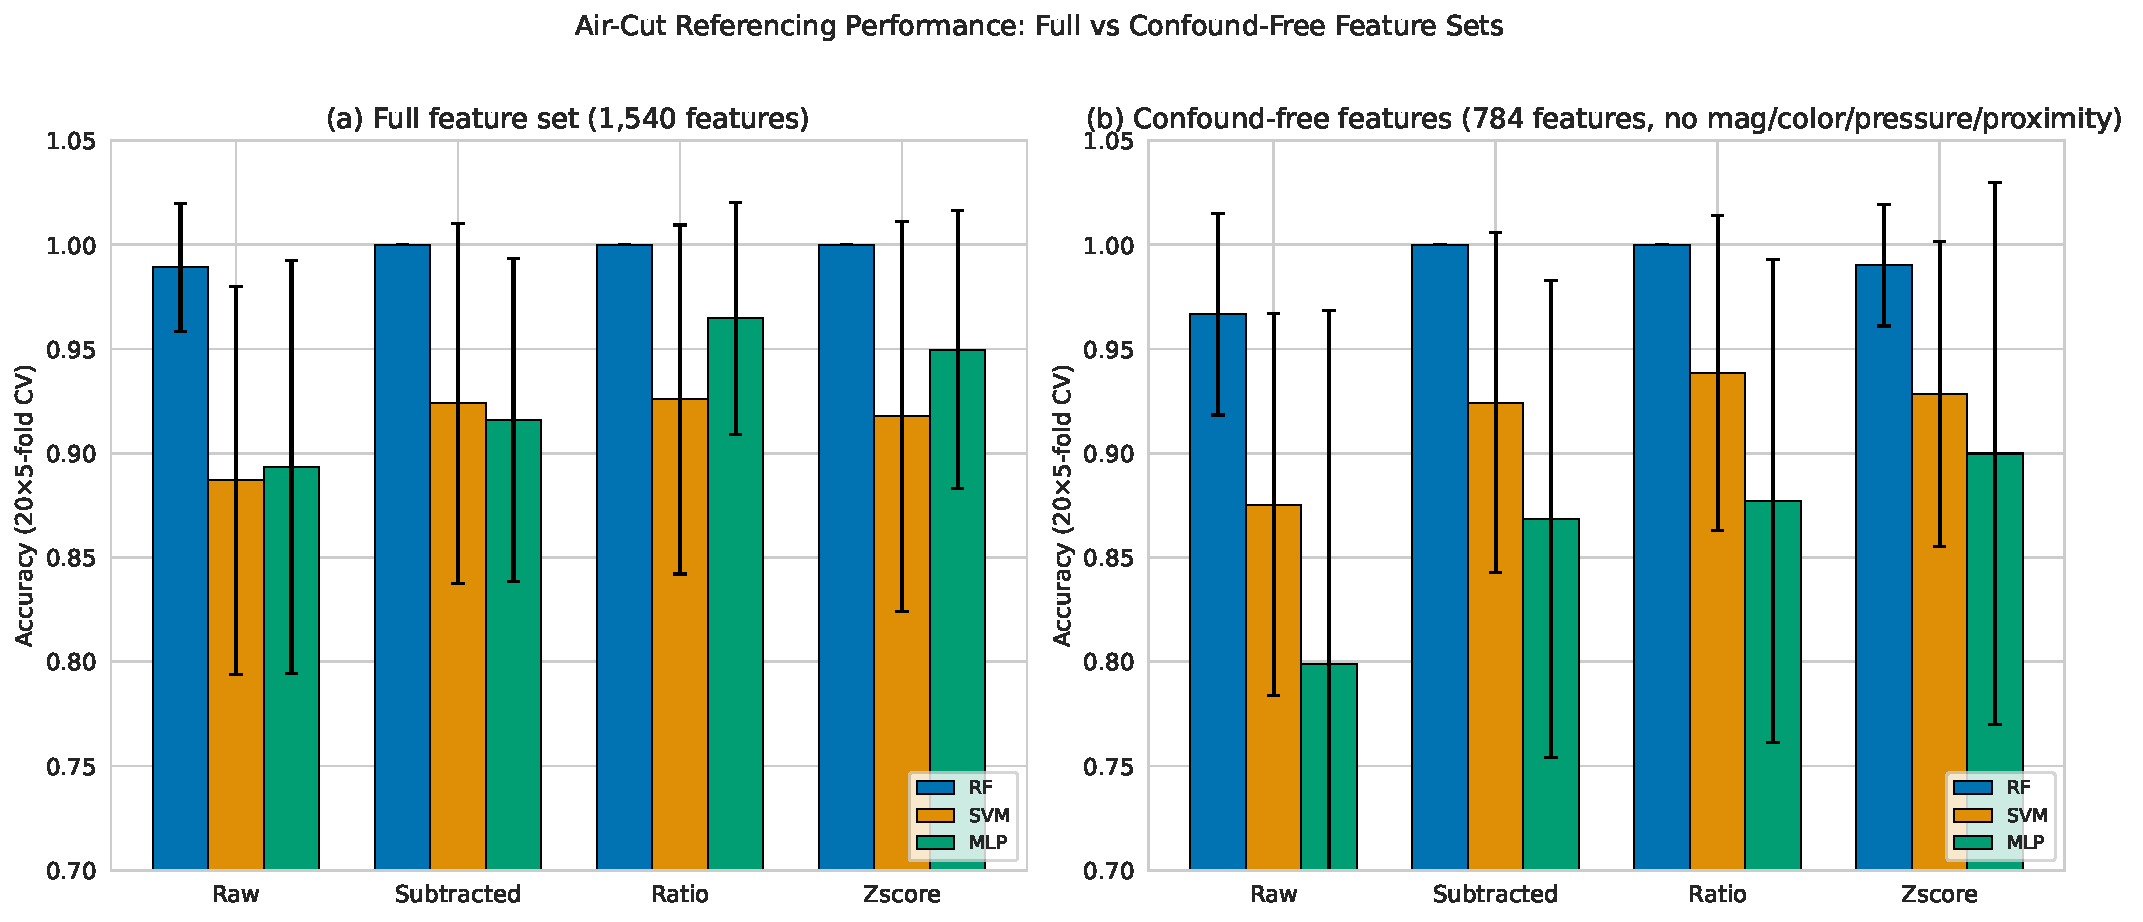
\includegraphics[width=\textwidth]{figures/fig20_confound_free_comparison.pdf}
    \caption{Air-cut referencing performance comparison. Left: full 1{,}540-feature set including position-confounded magnetometer channels. Right: 784 confound-free features (no magnetometer, color, pressure, proximity). The raw-vs-referenced gap widens in the confound-free condition, particularly for SVM and MLP, demonstrating that referencing provides genuine benefit beyond position encoding. (Panel regenerated on the corrected 784-feature set; subtracted/ratio RF reach 100\% and z-score RF 99.0\%, vs.\ raw 96.7\%.)}
    \label{fig:confound_free_viz}
\end{figure}

In the confound-free condition (right panel), the gap between raw and referenced methods widens. For RF, raw drops from $\sim$99\% to 96.7\% while the subtracted and ratio methods stay at 100\% and z-score at 99.0\%. For MLP, raw drops to $\sim$80\% while z-score recovers to 90\%. The position-confounded channels were inflating the raw baseline; removing them reveals the true (more modest) magnitude of the air-cut referencing benefit.

\subsection{Mutual Information Decomposition}\label{sec:mi}

To quantify how much of each feature's discriminative content is genuinely class-related versus position-encoded, we compute mutual information (MI) between each feature and three targets: the class label, the run order, and a position proxy defined as the first principal component of the magnetometer feature subspace. The position proxy explains 21.2\% of magnetometer variance and serves as a continuous proxy for the workspace region traversed during a run.

\begin{table}[H]
\caption{Mutual information by sensor channel type. MI is reported in bits; the maximum possible MI between a feature and a 3-class label is $\log_2 3 = 1.585$ bits. The ``\%pos/cls'' column reports the ratio of position-MI to class-MI, where values near or above 100\% indicate that the feature's class-discriminative content is fully accounted for by workspace position.}\label{tab:mi_decomposition}
\centering
\begin{tabular}{lccccc}
\toprule
\textbf{Channel Type} & \textbf{MI(class)} & \textbf{MI(order)} & \textbf{MI(pos)} & \textbf{\%pos/cls} & \textbf{N} \\
\midrule
Magnetometer  & 0.455 & 0.110 & 0.503 & 110.5\% & 252 \\
Accelerometer & 0.247 & 0.109 & 0.305 & 123.3\% & 252 \\
Gyroscope     & 0.225 & 0.129 & 0.257 & 114.2\% & 252 \\
Vibration RMS & 0.517 & 0.078 & 0.574 & 111.1\% & 84 \\
Temperature   & 0.241 & 0.325 & 0.256 & 106.2\% & 84 \\
Pressure      & 0.538 & 0.153 & 0.431 & 80.0\%  & 84 \\
Proximity     & 0.326 & 0.273 & 0.337 & 103.2\% & 84 \\
Color         & 0.323 & 0.204 & 0.340 & 105.4\% & 336 \\
Electrical    & 0.179 & 0.024 & 0.180 & 100.3\% & 112 \\
\bottomrule
\end{tabular}
\end{table}

\begin{figure}[H]
    \centering
    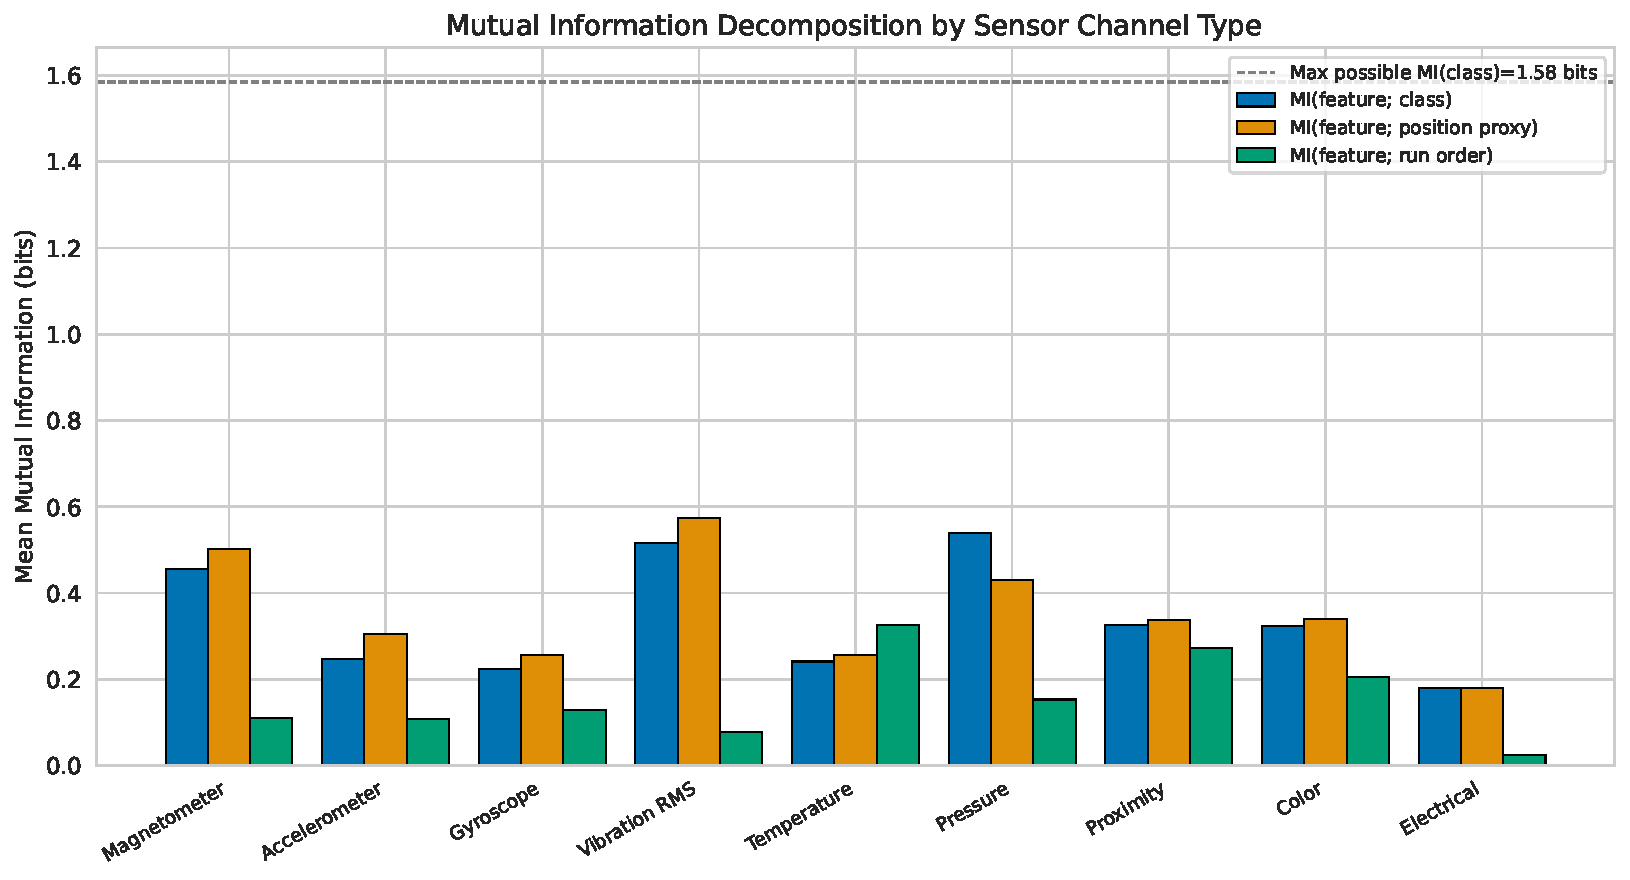
\includegraphics[width=0.85\textwidth]{figures/fig22_mi_decomposition.pdf}
    \caption{Mutual information decomposition by sensor channel type. For nearly all sensor types, MI(feature; position proxy) is comparable to or exceeds MI(feature; class), indicating that workspace position accounts for the majority of class-discriminative content.}
    \label{fig:mi_decomposition}
\end{figure}

The MI analysis quantitatively confirms the position-encoding finding from Section~\ref{sec:physics}. For nearly every channel type, MI(feature; position) is comparable to or exceeds MI(feature; class), with ratios above 100\% indicating that position information saturates the class signal. Pressure (the only ratio below 100\%) carries class information beyond position, but this reflects barometric session-day variation rather than process physics. Of the 1{,}540 features, 362 have MI(class) $> 0.5$~bits, 422 have MI(position) $> 0.5$~bits, and \textbf{321 of those (89\%) overlap}, meaning that the vast majority of high-class-information features are also high-position-information features. Temperature has the highest MI(order) value (0.325 bits), reflecting the within-class warming drift identified in Section~\ref{sec:discussion}; this is one of the few channels where information is genuinely tied to recording chronology rather than class structure or position.

One methodological caveat applies. The position proxy is defined as the first principal component of the magnetometer feature subspace, which makes the MI(magnetometer feature; position) measurement slightly circular by construction (the magnetometer features are partly being correlated with a transformation of themselves). This circularity inflates the magnetometer ratio (110.5\%) by an unknown amount. The more consequential cross-sensor finding is unaffected, however: accelerometer (123.3\%), gyroscope (114.2\%), vibration RMS (111.1\%), proximity (103.2\%), color (105.4\%), and electrical (100.3\%) channels all exceed the 100\% threshold despite being computed independently of the magnetometer subspace, demonstrating that workspace position dominates the discriminative content across the entire sensor array.

\subsection{Bayesian Posterior Analysis}\label{sec:bayesian}

The frequentist analyses (Friedman test, bootstrap CIs, Cliff's delta) provide significance testing under various assumptions, but each is constrained by the ceiling effects in the referenced methods (which achieve 100\% on every fold). To complement these, we model the per-fold accuracy as a Beta-Binomial conjugate problem: with 100 cross-validation folds totaling 1{,}020 test predictions per method, we compute the posterior $\text{Beta}(1 + n_\text{correct}, 1 + n_\text{incorrect})$ on the underlying accuracy, then sample 100{,}000 draws to compute posterior probabilities of difference. The $\text{Beta}(1, 1)$ prior is uniform on $[0, 1]$ and is therefore non-informative; with $n = 1{,}020$ predictions per method, the posterior is dominated by the likelihood and the choice of prior has negligible effect (sensitivity to a Jeffreys $\text{Beta}(0.5, 0.5)$ prior shifts the posterior medians by $< 0.05$ percentage points).

\begin{table}[H]
\caption{Bayesian posterior analysis (Beta-Binomial conjugate, $\text{Beta}(1, 1)$ prior). For each method, $n_\text{correct}/n_\text{total}$ across 100 CV folds gives the likelihood. Posterior 95\% credible intervals (CrI) and posterior probability of exceeding raw are computed from 100{,}000 samples.}\label{tab:bayesian}
\centering
\begin{tabular}{lcccc}
\toprule
\textbf{Method} & \textbf{$n_\text{correct}/n_\text{total}$} & \textbf{Posterior median} & \textbf{95\% CrI} & \textbf{$P(>\text{raw})$} \\
\midrule
Raw        & 1009/1020 & 98.86\% & [98.08\%, 99.39\%] & --- \\
Subtracted & 1020/1020 & 99.93\% & [99.64\%, 100.00\%] & 0.9997 \\
Ratio      & 1020/1020 & 99.93\% & [99.63\%, 100.00\%] & 0.9998 \\
Z-score    & 1020/1020 & 99.93\% & [99.64\%, 100.00\%] & 0.9998 \\
\bottomrule
\end{tabular}
\end{table}

\begin{figure}[H]
    \centering
    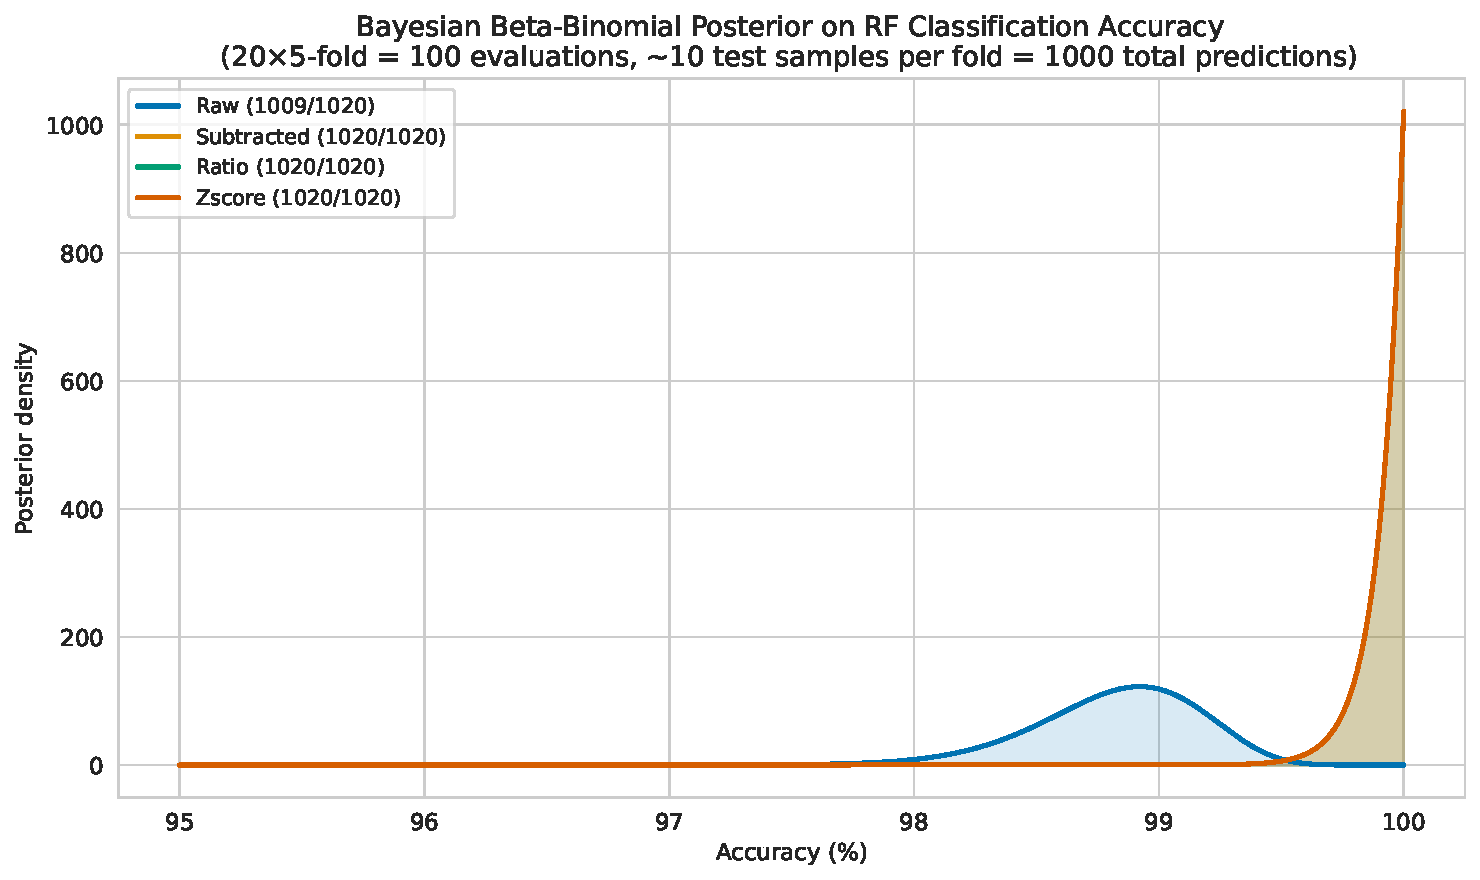
\includegraphics[width=0.75\textwidth]{figures/fig21_bayesian_posterior.pdf}
    \caption{Bayesian Beta-Binomial posterior densities on RF classification accuracy for each isolation method. The raw method's posterior is centered at 98.86\% with non-trivial mass below 99\%, while the three referenced methods concentrate above 99.6\%. The posterior probability that any referenced method exceeds raw is $\geq 0.9997$.}
    \label{fig:bayesian_posterior}
\end{figure}

The posterior accuracy difference between any referenced method and raw has median $1.05\%$ with a 95\% credible interval of $[0.46\%, 1.84\%]$, and $P(\text{referenced} > \text{raw}) \geq 0.9997$. This Bayesian framing provides three advantages over the frequentist tests: (1)~it produces a properly bounded credible interval despite the ceiling effect in the referenced methods, replacing the degenerate frequentist CI $[1.000, 1.000]$ with the principled $[0.9964, 0.99997]$; (2)~it gives a direct probability statement about the comparison rather than a $p$-value against a null hypothesis; and (3)~it makes explicit that the magnitude of the effect, while small in absolute terms ($\sim$1 percentage point), is overwhelmingly likely to be a real positive effect rather than noise. One caveat applies. The Beta--Binomial model treats the 1{,}020 fold-level predictions as independent Bernoulli trials, but they derive from only 51 runs evaluated $\sim$20 times each (raw's 11 errors trace largely to a single borderline run). The effective sample size is therefore closer to 51 than 1{,}020, so the credible interval and $P(\text{referenced} > \text{raw})$ should be read as optimistic upper bounds on certainty rather than calibrated probabilities; the run-level Cliff's-delta analysis, which localizes the effect to one run, is the more conservative summary.

\subsection{Temporal Fingerprints}\label{sec:fingerprints}

Figure~\ref{fig:fingerprint} shows the per-class temporal fingerprints of the most discriminative position-proxy channel (frame\_r2.Mx) across the 20 temporal bins, with each toolpath type's individual runs and mean~$\pm$~std, in both the raw-active and air-cut-subtracted representations.

\begin{figure}[H]
    \centering
    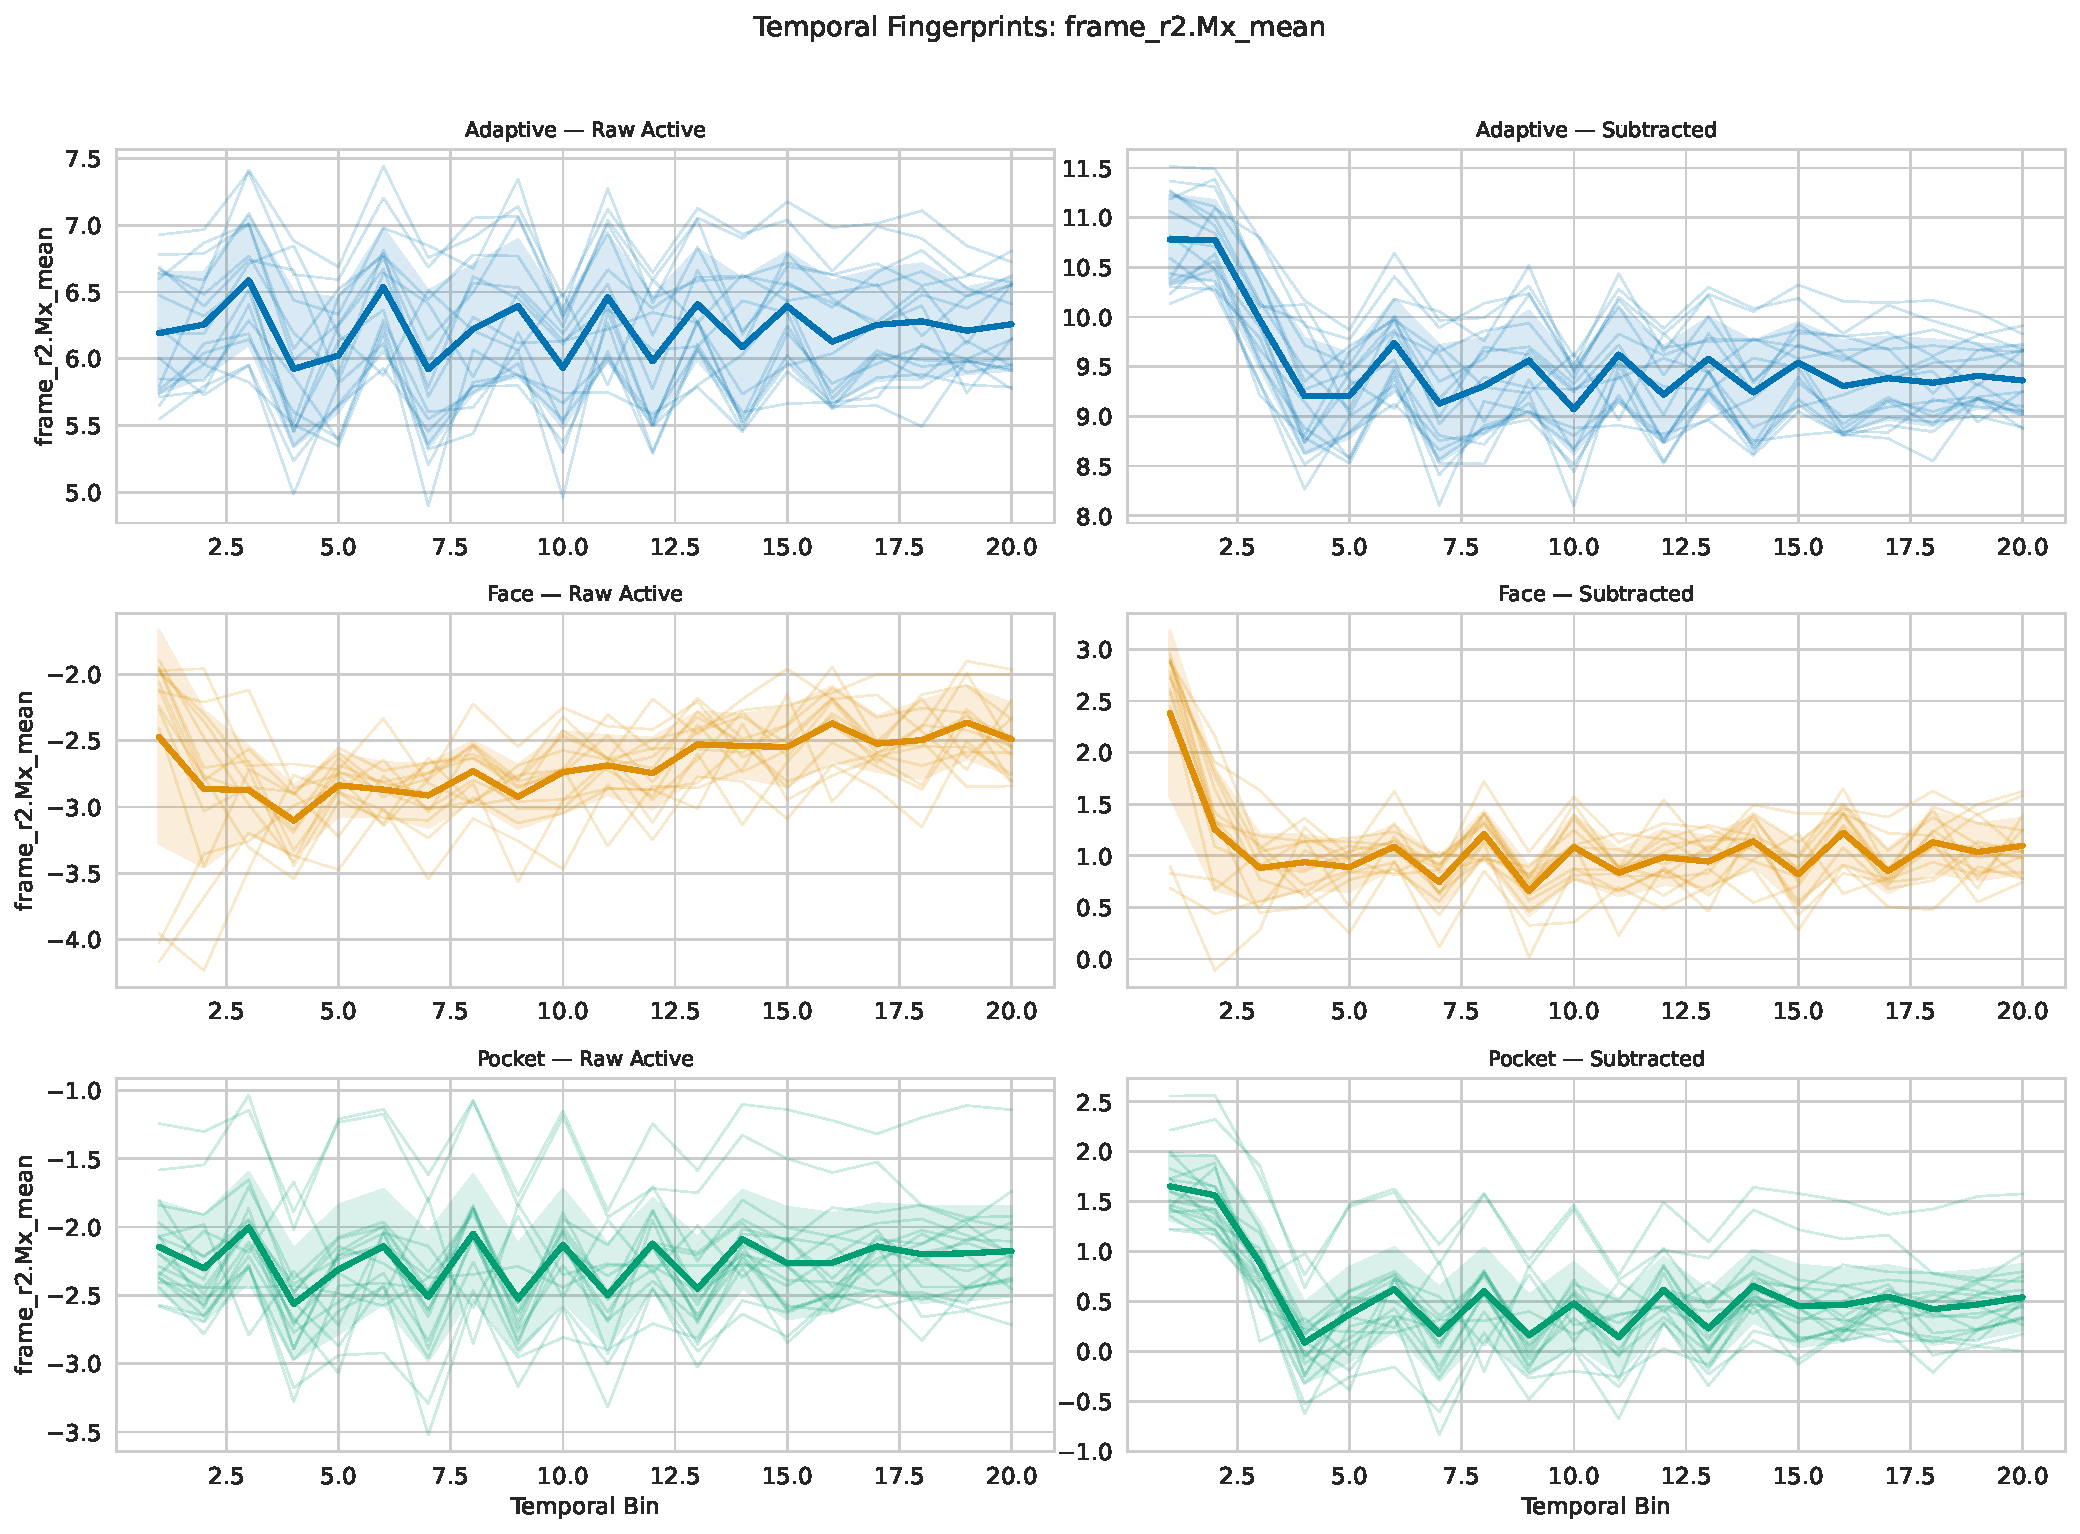
\includegraphics[width=0.9\textwidth]{figures/fig6_temporal_fingerprint.pdf}
    \caption{Temporal fingerprints of the top-ranked position-proxy channel (frame\_r2.Mx mean) across 20 temporal bins, by toolpath type (rows: adaptive, facing, pocketing) and representation (left: raw active; right: air-cut subtracted). Thin lines are individual runs; the bold line and shaded band are the per-type mean~$\pm$~one standard deviation. The three types occupy distinct magnetometer ranges---a workspace-position effect (Section~\ref{sec:physics})---and air-cut subtraction (right column) compresses the inter-type offsets while retaining a residual separation.}
    \label{fig:fingerprint}
\end{figure}

Figure~\ref{fig:fingerprint_overlay} presents the temporal fingerprint overlay, showing how the three toolpath types produce distinct quasi-static sensor signal profiles across normalized program time.

\begin{figure}[H]
    \centering
    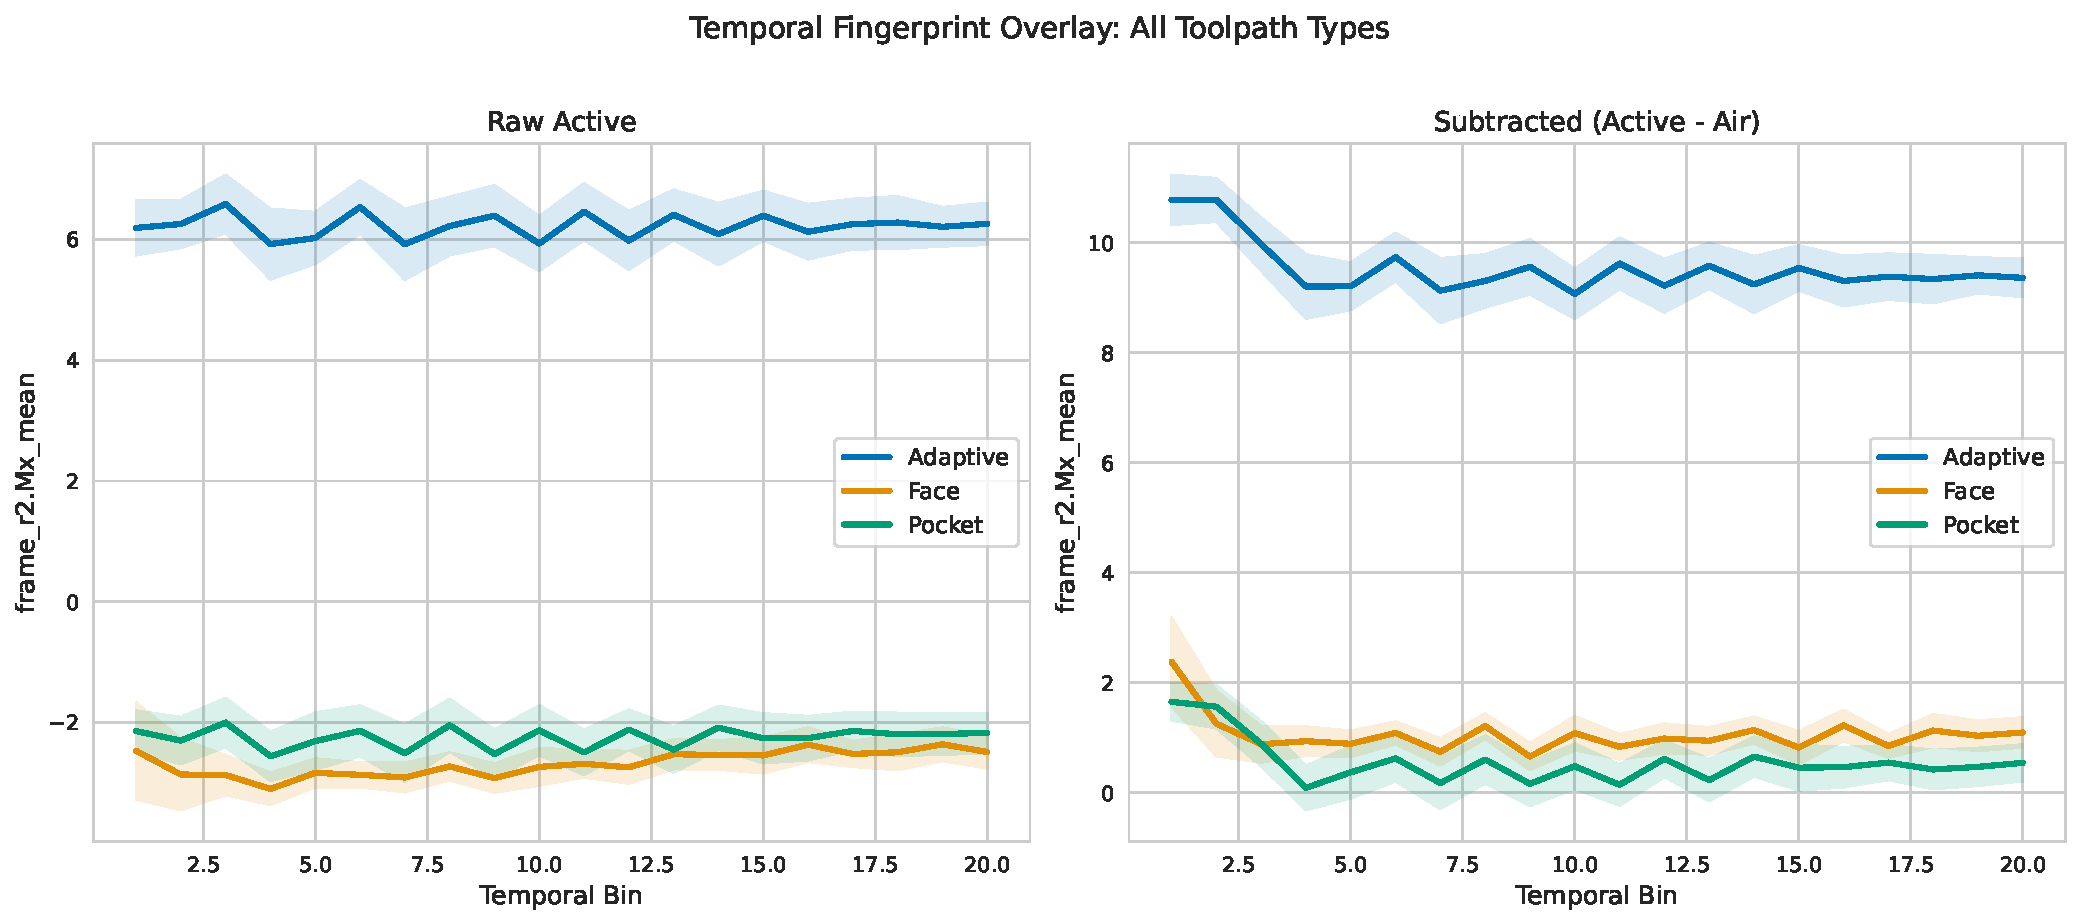
\includegraphics[width=0.85\textwidth]{figures/fig6b_temporal_overlay.pdf}
    \caption{Temporal fingerprint overlay for all three toolpath types. Left: raw active signals. Right: subtracted (air-cut referenced) signals. Shaded regions: $\pm 1$ std. The distinct separation between classes persists after subtraction. Note that these profiles reflect quasi-static motion envelopes rather than cutting vibration dynamics (Section~\ref{sec:sampling}).}
    \label{fig:fingerprint_overlay}
\end{figure}

Adaptive clearing produces the highest absolute magnetometer values (reflecting its workspace location) with gradual temporal variation, while facing and pocketing occupy a different region with more temporal structure. After air-cut subtraction (right panel), the inter-class separation is reduced but still present, confirming that some discriminative information survives the referencing process and is not purely position-dependent.

\subsection{Generalization Analysis}

Table~\ref{tab:generalization} reports leave-$K$-runs-out CV results.

\begin{table}[H]
\caption{Leave-$K$-runs-out accuracy (RF). For $K \geq 2$, results are averaged over 100 random combinations.}\label{tab:generalization}
\centering
\begin{tabular}{lccc}
\toprule
\textbf{Method} & \textbf{$K = 1$} & \textbf{$K = 2$} & \textbf{$K = 3$} \\
\midrule
Raw        & $100.0 \pm 0.0$ & $99.5 \pm 5.0$ & $99.0 \pm 5.7$ \\
Subtracted & $100.0 \pm 0.0$ & $100.0 \pm 0.0$ & $100.0 \pm 0.0$ \\
Ratio      & $100.0 \pm 0.0$ & $100.0 \pm 0.0$ & $100.0 \pm 0.0$ \\
Z-score    & $100.0 \pm 0.0$ & $100.0 \pm 0.0$ & $100.0 \pm 0.0$ \\
\bottomrule
\end{tabular}
\end{table}

Raw features degrade slightly at $K = 3$ (99.0\%), while all referenced methods maintain 100\%, consistent with the repeated CV finding that air-cut referencing improves robustness.

\subsection{Harder Classification Tasks}

To probe the limits of the methodology beyond the easy three-class task, we evaluate several more challenging classification scenarios.

\subsubsection{Six-Class Classification (Toolpath $\times$ Condition)}

Combining the 55 air-cut and 51 active-cut runs into a six-class problem (3 toolpath types $\times$ 2 cutting conditions), the RF classifier achieves $99.1\% \pm 1.8\%$ accuracy. This demonstrates that sensor features can simultaneously distinguish both the toolpath type and the cutting condition (air vs.\ active), with near-perfect separability.

\subsubsection{Air vs.\ Active Discrimination}

Binary classification of air-cut vs.\ active-cut runs (ignoring toolpath type) achieves $99.0\% \pm 1.9\%$ accuracy, confirming that material engagement produces a detectable change in sensor signatures across all toolpath types. Per-toolpath binary discrimination (air vs.\ active within each type) achieves 100\% for all three types.

\subsubsection{Cross-Condition Transfer}

Whether models transfer across cutting conditions is a direct test of the air-cut referencing hypothesis. We train an RF classifier on \textit{air-cut data only} (55 runs, 3 toolpath classes) and test on \textit{active-cut data} (51 runs):

\begin{table}[H]
\caption{Cross-condition transfer accuracy. Models trained on one condition are tested on the other without retraining.}\label{tab:cross_condition}
\centering
\begin{tabular}{lcc}
\toprule
\textbf{Transfer Direction} & \textbf{Accuracy (\%)} & \textbf{Train / Test} \\
\midrule
Air $\rightarrow$ Active   & 37.3 & 55 / 51 \\
Active $\rightarrow$ Air   & 40.0 & 51 / 55 \\
\bottomrule
\end{tabular}
\end{table}

Both transfer directions achieve near-chance accuracy ($\sim$37--40\% vs.\ 33\% random baseline), demonstrating that raw sensor features learned from one cutting condition do not transfer to the other. This result has two implications: (1)~it confirms that the air and active sensor signals are fundamentally different, with the machine dynamics (captured by air cuts) and process dynamics (added by active cuts) producing distinct feature distributions; and (2)~it motivates the air-cut referencing methodology, since the process component isolated by subtraction/normalization may be more transferable than the raw signal.

\subsubsection{Leave-One-Type-Out: Unknown Toolpath Detection}

We train a binary classifier on two toolpath types and examine its behavior when presented with the unseen third type. Since the held-out class was not in the training data, the classifier must assign it to one of the known classes.

\begin{table}[H]
\caption{Leave-one-type-out analysis. An RF classifier trained on two toolpath types is applied to the unseen third type. ``Predicted as'' shows how the unknown type is classified; ``Confidence'' reports the RF posterior probability.}\label{tab:loto}
\centering
\begin{tabular}{llcc}
\toprule
\textbf{Held Out} & \textbf{Predicted As} & \textbf{Mean Conf.} & \textbf{Min Conf.} \\
\midrule
Adaptive (17)  & Pocket: 17/17    & $0.77 \pm 0.05$ & 0.67 \\
Face (15)      & Pocket: 15/15    & $0.79 \pm 0.04$ & 0.71 \\
Pocket (19)    & Adaptive: 16, Face: 3   & $0.63 \pm 0.06$ & 0.52 \\
\bottomrule
\end{tabular}
\end{table}

When adaptive or face toolpaths are held out, the classifier consistently predicts ``pocket'' with moderate confidence (0.67--0.79). When pocket is held out, predictions split between adaptive (84\%) and face (16\%) with lower confidence (min 0.52). The reduced confidence for unknown types suggests that a confidence-thresholding approach could potentially detect novel toolpath types, a direction for future work in anomaly detection.


\section{Ablation Study}\label{sec:ablation}

To understand which components of the sensing and feature extraction pipeline are critical for classification performance, we conduct a comprehensive ablation study. All ablation experiments use the RF classifier with the raw isolation method (the best-performing configuration without PCA).

\subsection{Sensor Group Ablation}

Table~\ref{tab:sensor_ablation} reports classification accuracy when restricting the feature set to individual sensor groups.

\begin{table}[H]
\caption{Classification accuracy by sensor group. ``All'' uses all 110 sensor channels. Individual Arduino modules use 17 channels each. Electrical uses 8 current sensors.}\label{tab:sensor_ablation}
\centering
\begin{tabular}{lcc}
\toprule
\textbf{Sensor Group} & \textbf{Accuracy (\%)} & \textbf{Features} \\
\midrule
All sensors              & $100.0 \pm 0.0$ & 1{,}540 \\
Arduino (all 6 modules)  & $100.0 \pm 0.0$ & 1{,}428 \\
y\_bed\_\_3              & $100.0 \pm 0.0$ & 238 \\
frame\_l2                & $98.0 \pm 4.0$ & 238 \\
y\_bed\_\_4              & $98.0 \pm 4.0$ & 238 \\
frame\_r2                & $96.0 \pm 4.9$ & 238 \\
spindle2                 & $96.0 \pm 4.9$ & 238 \\
frame\_l3                & $94.0 \pm 8.0$ & 238 \\
Electrical (current only) & $76.5 \pm 12.4$ & 112 \\
\bottomrule
\end{tabular}
\end{table}

The y\_bed\_\_3 sensor module alone achieves 100\% accuracy with only 238 features, demonstrating that a single well-placed IMU on the machine bed is sufficient for perfect toolpath classification. This finding has practical significance: a minimal sensor deployment of one IMU near the workpiece can match the performance of the full 10-sensor array. The electrical current sensors alone achieve only 76.5\% accuracy (112 features; corrected from an earlier leaked figure of 96.0\%/350 features that had folded IMU channels into the electrical set, Section~\ref{sec:results}), confirming that motor-current monitoring is substantially less discriminative than vibration sensing on this task---consistent with the near-constant spindle current under the shallow UHMW-PE cut.

\subsection{Feature Statistic Ablation}

Table~\ref{tab:stat_ablation} examines how many summary statistics per temporal bin are needed.

\begin{table}[H]
\caption{Classification accuracy as a function of the number of summary statistics computed per temporal bin.}\label{tab:stat_ablation}
\centering
\begin{tabular}{lcc}
\toprule
\textbf{Statistic Set} & \textbf{Accuracy (\%)} & \textbf{Features} \\
\midrule
Mean + RMS (2 stats)             & $98.0 \pm 4.0$ & 440 \\
Mean + RMS + Std (3 stats)       & $98.0 \pm 4.0$ & 660 \\
All 7 statistics                 & $100.0 \pm 0.0$ & 1{,}540 \\
\bottomrule
\end{tabular}
\end{table}

Even with only two statistics (mean and RMS), classification accuracy reaches 98\%, indicating that the temporal bin means and RMS values capture most of the discriminative information. The full 7-statistic set adds higher-order statistics (skewness, kurtosis) that contribute the final 2\% improvement.

\subsection{Alignment Ablation: Temporal Binning vs.\ Whole-Run Summary}

Table~\ref{tab:alignment_ablation} compares the temporal binning approach against whole-run summary statistics.

\begin{table}[H]
\caption{Classification accuracy for temporal binning ($B = 20$, aggregated to mean + std across bins) vs.\ whole-run summary statistics (no temporal structure).}\label{tab:alignment_ablation}
\centering
\begin{tabular}{lcc}
\toprule
\textbf{Approach} & \textbf{Accuracy (\%)} & \textbf{Features} \\
\midrule
Temporal binning (20 bins)  & $100.0 \pm 0.0$ & 1{,}540 \\
Whole-run summary           & $98.0 \pm 4.0$ & 770 \\
\bottomrule
\end{tabular}
\end{table}

Temporal binning outperforms whole-run summary by 2 percentage points. While modest, this confirms that the temporal evolution of sensor statistics carries discriminative information. The temporal approach also enables the fingerprint visualizations (Figure~\ref{fig:fingerprint}) that provide interpretable insight into how toolpath types differ.

\subsection{PCA Ablation}

Table~\ref{tab:pca_ablation} examines the effect of PCA dimensionality reduction across all three classifiers.

\begin{table}[H]
\caption{Classification accuracy (\%) vs.\ PCA component count, for all three classifiers with raw features. RF shows invariance to component count (all reduce to 88.2\%), while SVM and MLP exhibit different sensitivity patterns.}\label{tab:pca_ablation}
\centering
\begin{tabular}{lccc}
\toprule
\textbf{Components} & \textbf{RF} & \textbf{SVM} & \textbf{MLP} \\
\midrule
No PCA (1{,}540)  & $100.0 \pm 0.0$ & $90.0 \pm 6.3$ & $86.0 \pm 10.2$ \\
2                  & $90.2 \pm 0.4$ & $90.2 \pm 0.4$ & $58.9 \pm 2.2$ \\
3                  & $88.2 \pm 4.1$ & $90.2 \pm 6.3$ & $74.2 \pm 12.2$ \\
5                  & $88.2 \pm 4.1$ & $94.0 \pm 4.9$ & $76.2 \pm 10.5$ \\
10                 & $88.2 \pm 4.1$ & $92.0 \pm 7.5$ & $90.0 \pm 12.6$ \\
15                 & $88.2 \pm 4.1$ & $92.0 \pm 7.5$ & $92.0 \pm 7.5$ \\
20                 & $88.2 \pm 4.1$ & $92.0 \pm 7.5$ & $88.2 \pm 4.1$ \\
30                 & $88.2 \pm 4.1$ & $92.0 \pm 7.5$ & $80.5 \pm 13.8$ \\
\bottomrule
\end{tabular}
\end{table}

The PCA results reveal classifier-dependent behavior. RF accuracy drops to exactly 88.2\% for any number of PCA components from 3 to 30, because the leading principal components contain sufficient class-separating variance for the RF decision boundaries, and additional components add only noise within the PCA-reduced space. In contrast, SVM accuracy \textit{improves} with PCA to 5 components (94.0\%), likely because PCA removes irrelevant high-dimensional noise that the RBF kernel is sensitive to. MLP shows non-monotonic behavior, peaking at 15 components (92.0\%) before degrading due to overfitting in higher dimensions with only 51 training samples. These results demonstrate that dimensionality reduction interacts strongly with classifier choice, and that the ``PCA hurts RF'' finding should not be generalized to all classifiers.

\textbf{PCA misclassification analysis.} To explain why RF accuracy is invariant to PCA component count, we examined which individual samples are misclassified across all PCA configurations. The same 5--6 samples are misclassified in \textit{every} PCA setting (3 through 30 components): pocket150025\_001, pocket150025\_002, pocket150025\_012, face150025\_001, face150025\_010, and (in most settings) pocket150025\_006. These runs are consistently confused between the pocketing and facing classes. This confirms that the invariance is not a statistical artifact but reflects a genuine decision boundary: PCA projects the data into a subspace where these specific runs fall near the class boundary, and no amount of additional PCA dimensions resolves the ambiguity. Without PCA, the full 1{,}540-dimensional feature space provides sufficient redundancy for RF to correctly classify these borderline runs.

\subsection{Learning Curve}

Figure~\ref{fig:learning_curve} shows classification accuracy as a function of training set size.

\begin{figure}[H]
    \centering
    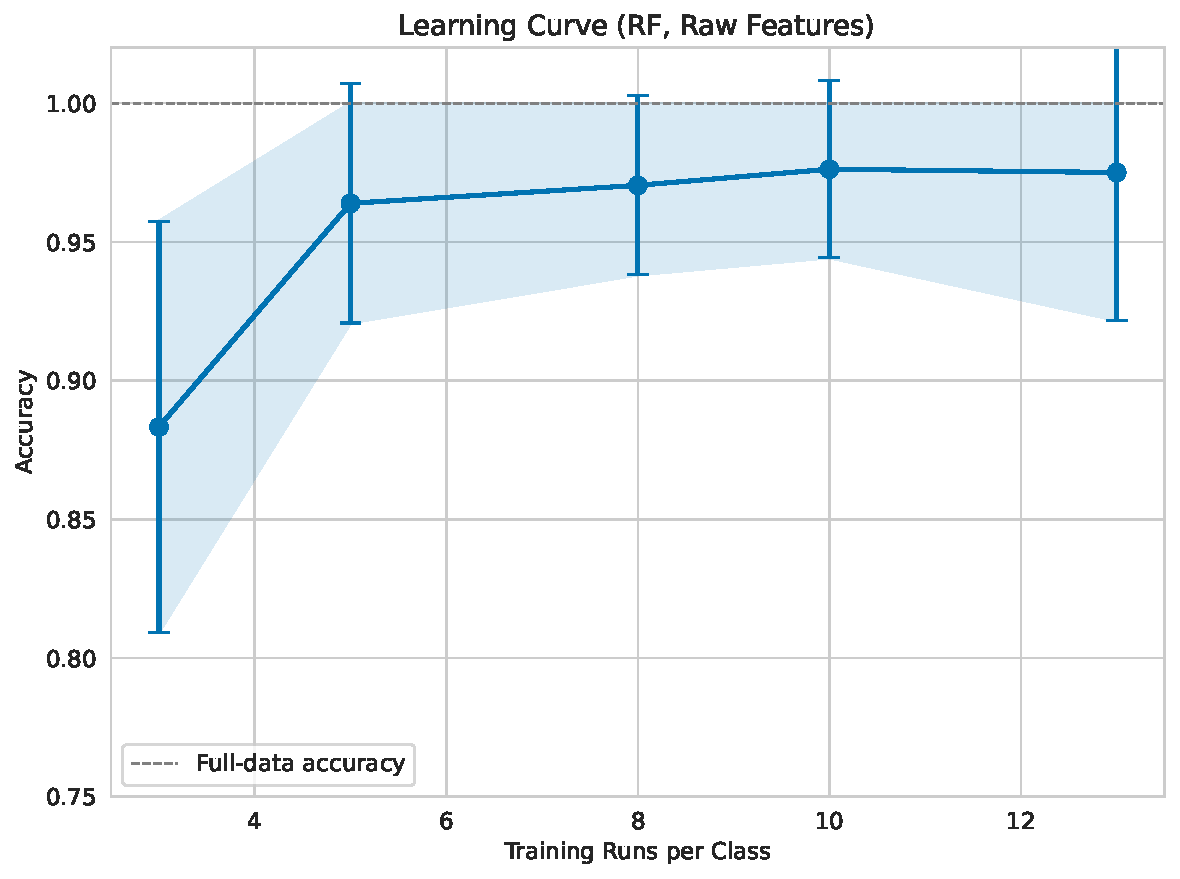
\includegraphics[width=0.7\textwidth]{figures/fig8_learning_curve.pdf}
    \caption{Learning curve: classification accuracy vs.\ number of training runs per class, using RF with raw features. Results are averaged over 10 random subsampling repeats.}
    \label{fig:learning_curve}
\end{figure}

With only 5 training runs per class (15 total), the classifier achieves 96.4\% accuracy. Performance plateaus above 8 runs per class at approximately 97\%. This steep learning curve demonstrates that the toolpath fingerprints are highly distinctive, requiring minimal training data.

\subsection{Sensor Contribution Heatmap}

Figure~\ref{fig:sensor_heatmap} provides a comprehensive view of how each sensor group performs across all four isolation methods.

\begin{figure}[H]
    \centering
    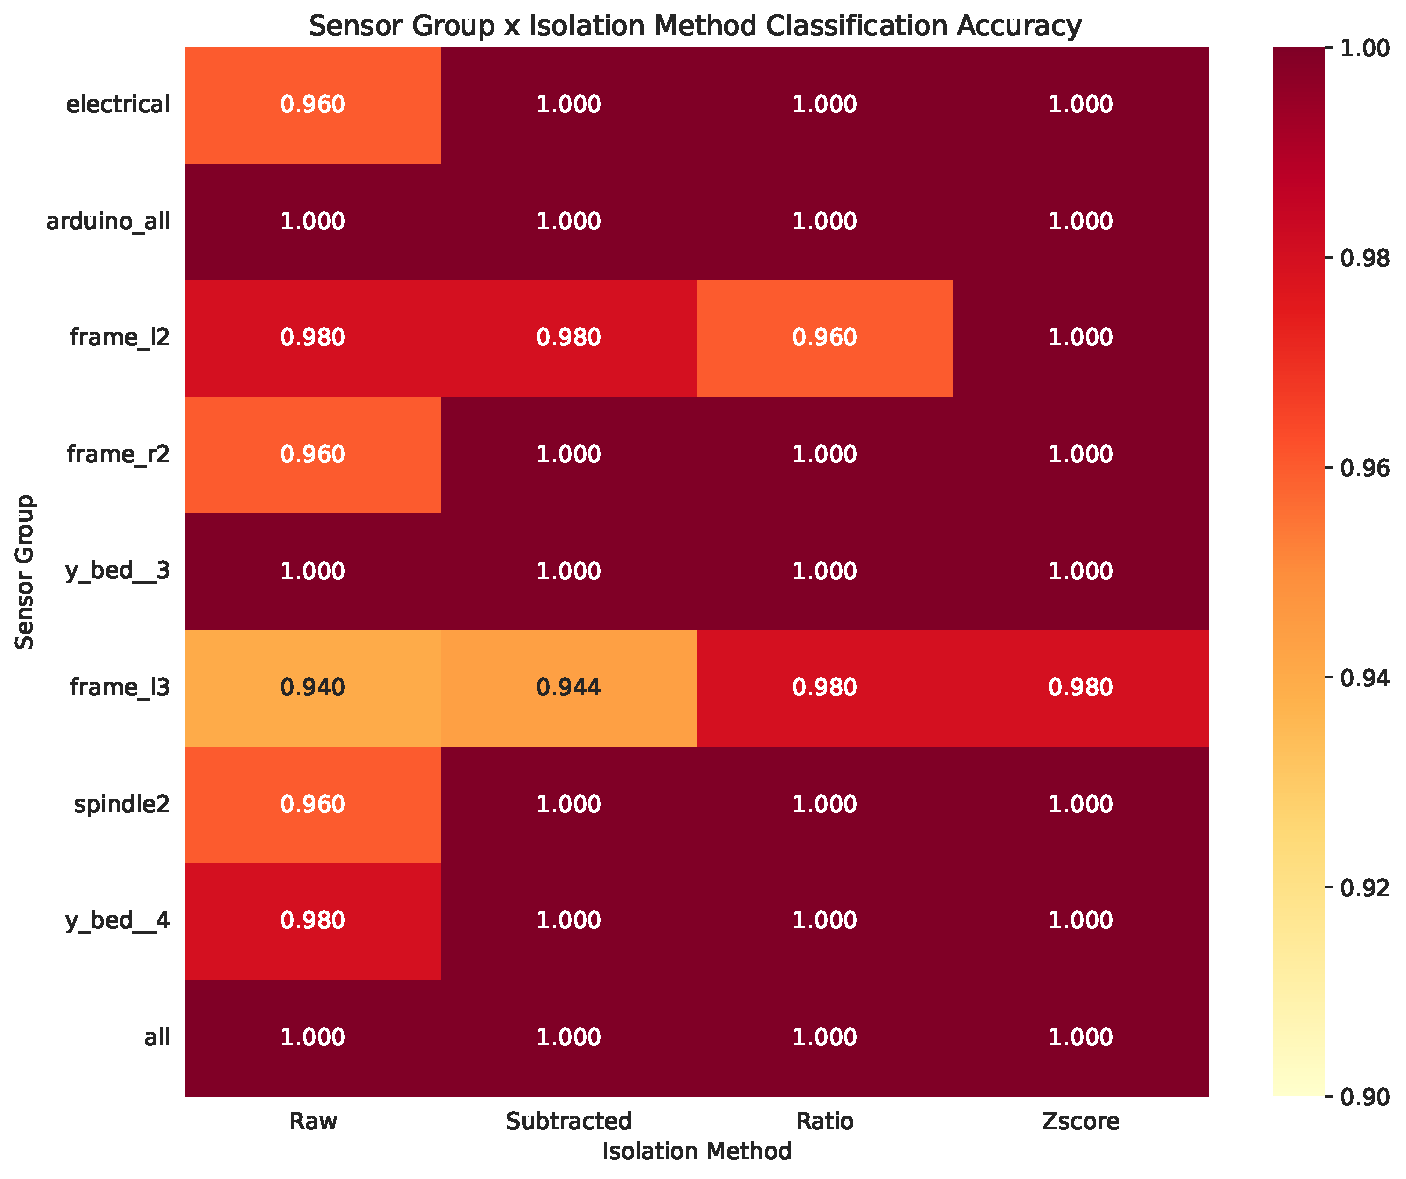
\includegraphics[width=0.85\textwidth]{figures/fig9_sensor_heatmap.pdf}
    \caption{Classification accuracy heatmap by sensor group (rows) and isolation method (columns), using the RF classifier. Darker colors indicate higher accuracy.}
    \label{fig:sensor_heatmap}
\end{figure}

The heatmap reveals that sensor performance is relatively consistent across isolation methods, suggesting that the sensor placement (physical position on the machine) is more important than the signal normalization strategy for this classification task.

\subsection{Noise Robustness}

To assess how sensitive each isolation method is to measurement noise, we add zero-mean Gaussian noise scaled by increasing fractions of the per-feature standard deviation and measure classification accuracy (Figure~\ref{fig:noise_robustness}).

\begin{figure}[H]
    \centering
    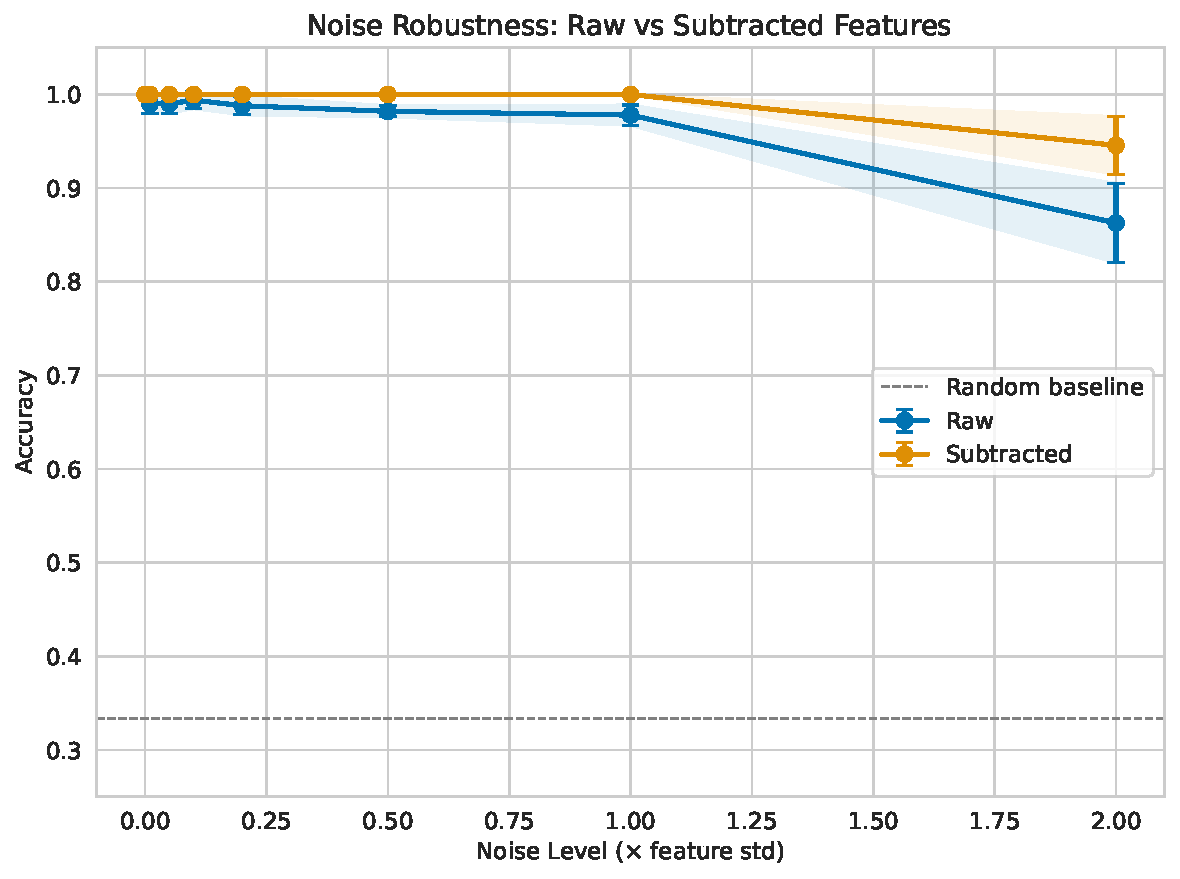
\includegraphics[width=0.7\textwidth]{figures/fig10_noise_robustness.pdf}
    \caption{Noise robustness: classification accuracy vs.\ additive Gaussian noise level (as a fraction of per-feature standard deviation). Subtracted features maintain 100\% accuracy up to $1.0\times$ noise, while raw features degrade to 97.8\%.}
    \label{fig:noise_robustness}
\end{figure}

Subtracted features are dramatically more noise-robust than raw features: they maintain 100\% accuracy up to $1.0\times$ noise (where the added noise equals the feature's natural standard deviation), while raw features degrade to 97.8\% at the same level. At $2.0\times$ noise, subtracted features still achieve 94.6\% vs.\ 86.3\% for raw. This result provides the strongest practical argument for air-cut referencing: the referenced features are substantially more resilient to sensor degradation, calibration drift, and environmental interference.

\subsection{Temporal Bin Importance}

Figure~\ref{fig:bin_importance} shows the accuracy impact of removing each of the 20 temporal bins.

\begin{figure}[H]
    \centering
    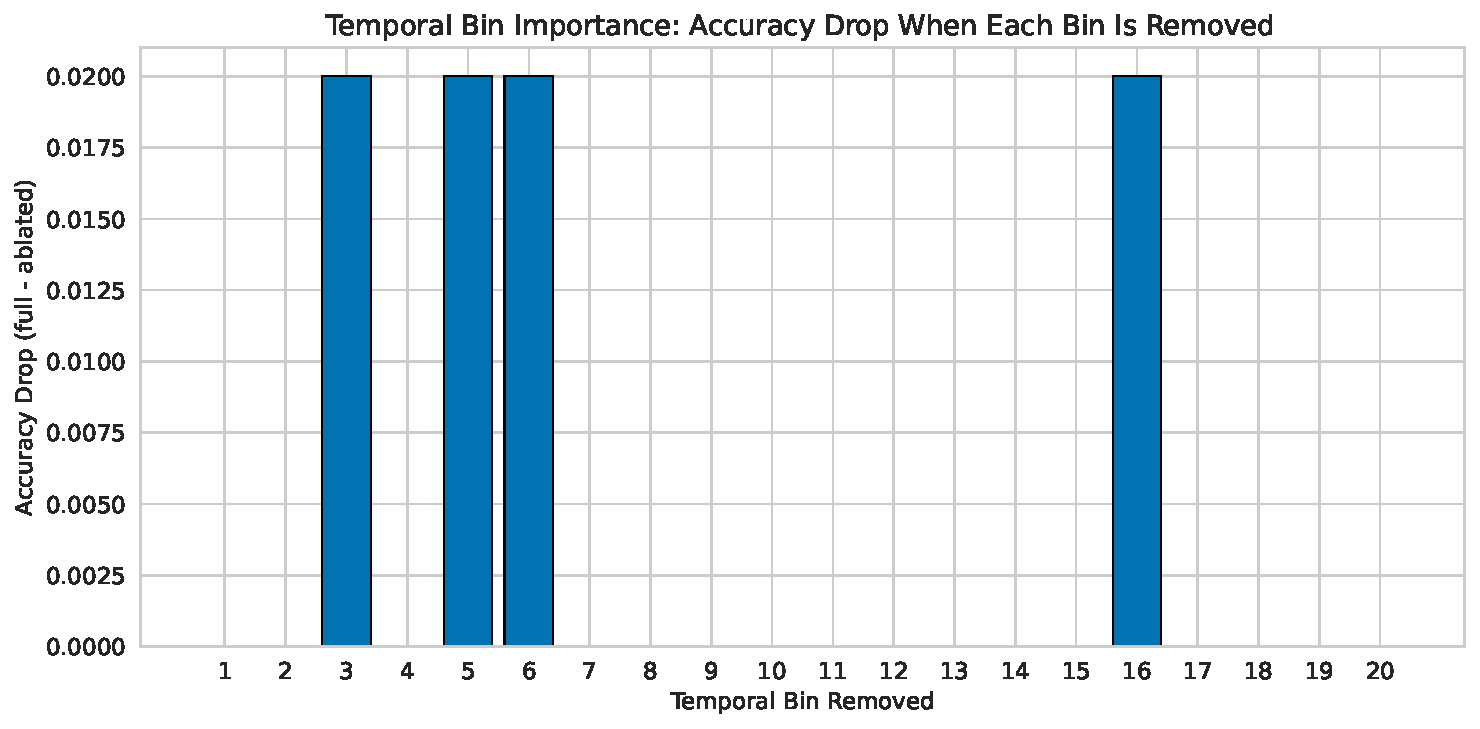
\includegraphics[width=0.85\textwidth]{figures/fig11_bin_importance.pdf}
    \caption{Accuracy drop when each temporal bin is removed (full accuracy minus leave-one-bin-out accuracy). Positive values indicate bins that contribute to classification. Bins 3, 5, 6, and 16 contribute most (each a 2-pp accuracy drop when removed).}
    \label{fig:bin_importance}
\end{figure}

Four bins share the largest impact: bins 3, 5, 6, and 16 (1-indexed), each causing a 2 percentage point drop to 98.0\% when removed. These correspond to approximately 10--30\% of normalized program time (the approach and early cutting phases) and 75--80\% (late cutting phase). The remaining 16 bins can each be removed without any accuracy loss, confirming that the temporal fingerprint's discriminative power is concentrated in specific program phases rather than distributed uniformly across the execution. This finding has practical implications: a coarser binning strategy focused on these critical phases could achieve comparable accuracy with fewer features.

Figure~\ref{fig:ablation_summary} summarizes the core ablation results in a composite figure.

\begin{figure}[H]
    \centering
    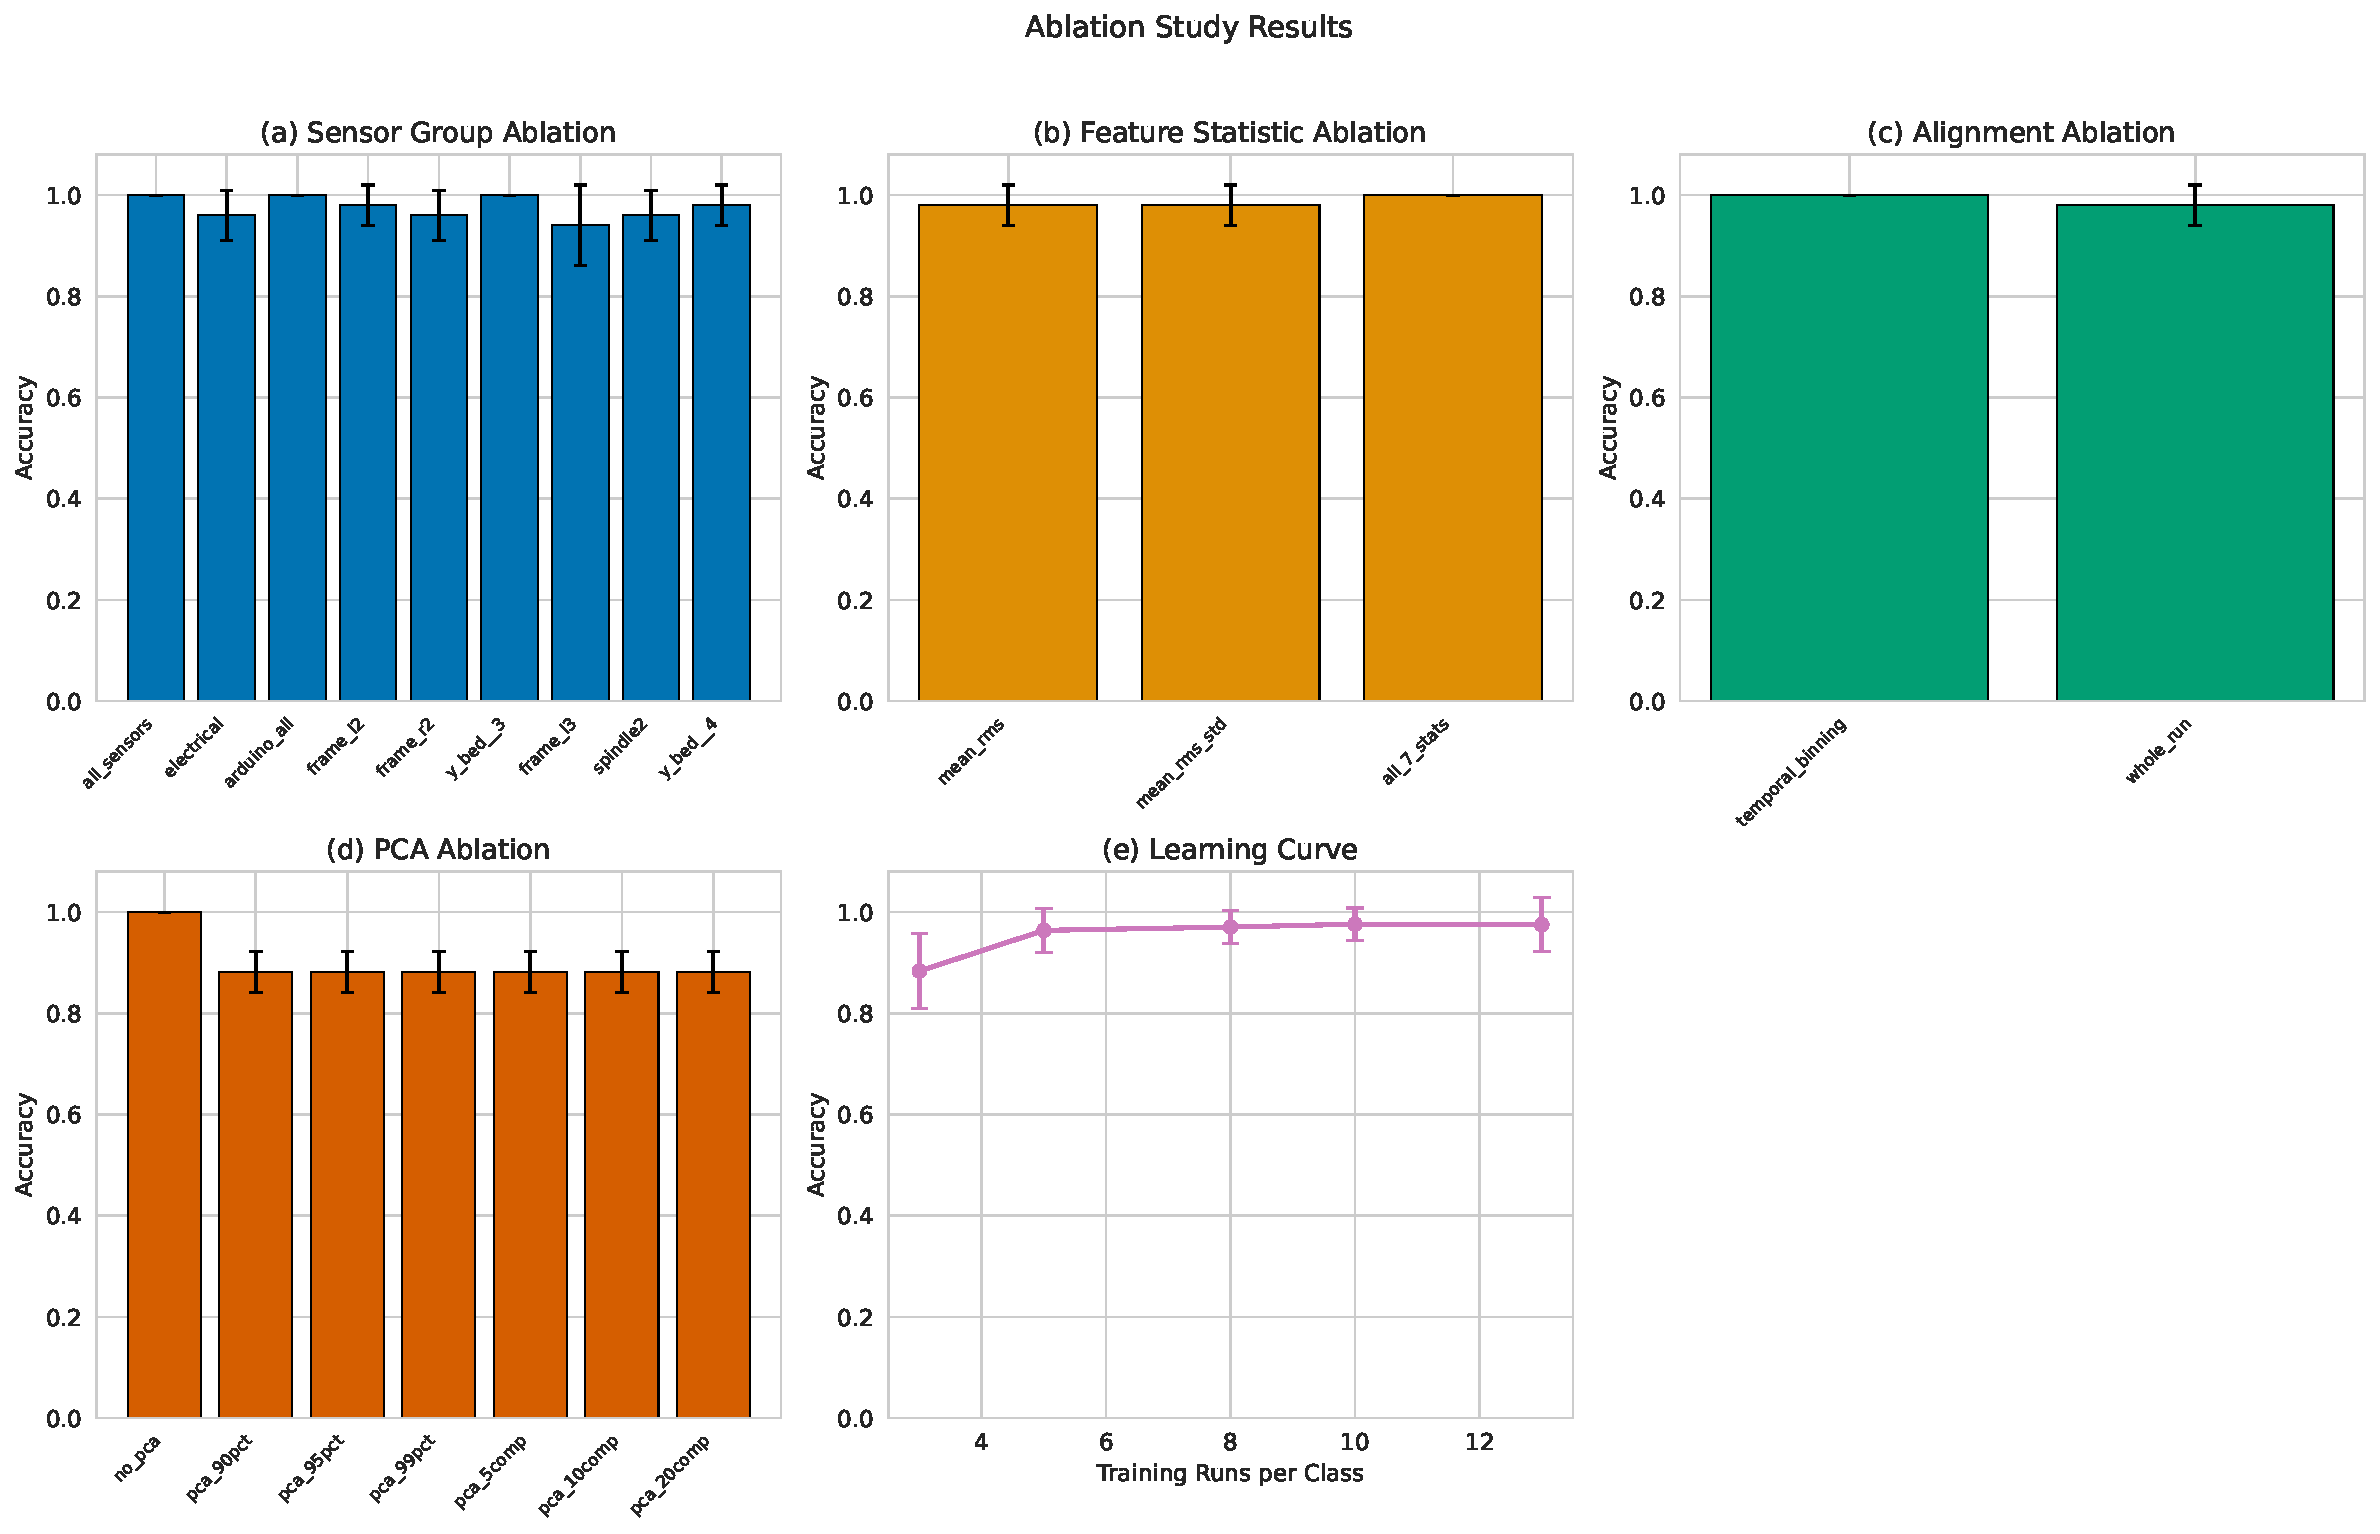
\includegraphics[width=\textwidth]{figures/fig7_ablation.pdf}
    \caption{Summary of core ablation studies: (a)~sensor group, (b)~feature statistics, (c)~alignment method, (d)~PCA configuration, (e)~learning curve.}
    \label{fig:ablation_summary}
\end{figure}


\section{Discussion}\label{sec:discussion}

\subsection{Task Difficulty and the Role of Trivial Baselines}

The trivial baseline analysis (Table~\ref{tab:trivial_baselines}) shows that the three toolpath types are distinguishable from program metadata alone, whether from G-code line range, mean axis position, or even row count. The 100\% RF accuracy achieved by our sensor features, while technically correct, therefore does not by itself demonstrate the value of sensor-based classification or air-cut referencing for this specific three-class task.

We report this finding because it establishes the true difficulty floor for this classification problem and prevents over-claiming. The sensor-based approach remains valuable for three reasons: (1) it works without access to program metadata, which may be unavailable or unreliable in deployment scenarios; (2) it provides the temporal fingerprint representation that offers interpretable physical insight; and (3) it establishes a methodology that transfers to harder discrimination tasks where metadata cannot help. The damaged-spindle detection result (Section~\ref{sec:damage}) demonstrates the third point. There the toolpath strategies are shared, so neither program metadata nor workspace position can separate the classes, yet the sensors reach 98.5\% accuracy using process-dynamics channels rather than the magnetometer position encoder; because the damaged runs are air-cuts, spindle condition and cutting engagement are confounded in that separation, which cannot be attributed to spindle condition alone.

\subsection{Effectiveness of Air-Cut Referencing}

Despite the easy task, three lines of evidence demonstrate a genuine contribution of air-cut referencing.

\textbf{Statistical significance (a consistency check, not the main evidence).} On the full feature set the air-cut effect is small and ceiling-bound. The Friedman test ($\chi^2 = 33.0$, $p < 10^{-6}$, $p_{\mathrm{Bonf}} = 0.011$) is significant, and the bootstrap CIs do not overlap (raw $[0.982, 0.994]$ vs.\ referenced $[1.000, 1.000]$). However, the gap is only $\sim$1~pp at a 100\% ceiling, Cliff's $\delta = 0.022$ is negligible, and the significance traces to a single recurrently-misclassified run. Cohen's $d$ is not meaningful here because the referenced methods have zero variance at the ceiling, so we do not interpret it. We therefore treat the full-feature tests as a consistency check and rest the case for air-cut referencing on the confound-free experiment (raw RF 96.7\% vs.\ subtracted/ratio 100\%) together with the noise-resilience and data-efficiency results below.

\textbf{Robustness.} Across 100 repeated CV evaluations, raw RF features occasionally misclassify (minimum fold accuracy 90\%), while referenced methods maintain perfect accuracy. Per-sample analysis traces this to a single borderline run (pocket150025\_001) that raw RF misclassifies 55\% of the time but all referenced methods classify correctly 100\% of the time.

\textbf{Noise resilience.} Subtracted features maintain 100\% accuracy up to $1.0\times$ additive noise (equal to the feature's natural standard deviation), while raw features degrade to 97.8\% (Figure~\ref{fig:noise_robustness}). At $2.0\times$ noise, the gap widens to 94.6\% vs.\ 86.3\%. This suggests that air-cut referencing would be particularly valuable in production environments with higher sensor noise, calibration drift, or environmental interference.

The two-way ANOVA shows that classifier choice ($\eta^2 = 0.17$) explains approximately $4\times$ more variance than isolation method ($\eta^2 = 0.04$), indicating that for this task, selecting the right classifier matters more than the referencing strategy.

For SVM and MLP classifiers, air-cut referencing provides 4--8 percentage point improvements in mean accuracy and reduces variance, suggesting it removes machine-specific baseline variation that these classifiers are sensitive to.

\subsection{Temporal Structure in Toolpath Fingerprints}

The temporal binning approach outperforms whole-run summary by 2 percentage points (100\% vs.\ 98\%), confirming that temporal structure carries discriminative information. The temporal fingerprint visualizations (Figure~\ref{fig:fingerprint}) reveal characteristic patterns: adaptive clearing produces gradual, continuous signal evolution; facing generates periodic oscillations corresponding to linear passes; and pocketing shows distinct phase transitions from contour passes.

The use of different G-code programs for air and active conditions necessitated temporal binning rather than point-by-point G-code-aligned subtraction. Despite this constraint, the temporal approach captures phase alignment (approach, cutting, retract) through normalized time binning. Future data collection with identical programs would enable a comparison of these approaches.

\subsection{What the Sensors Are Actually Detecting}

The physical interpretation analysis (Section~\ref{sec:physics}) shows that the dominant discriminative features are magnetometer channels that primarily encode \emph{workspace position} (proximity to motors and ferromagnetic structure) rather than \emph{cutting dynamics} (forces, vibrations, torque). This is the sensor-domain equivalent of the trivial position baseline; the classifier can distinguish toolpath types largely because the three programs move through different regions of the machine's workspace.

This observation has three implications:
\begin{itemize}
    \item \textbf{For this study}: the high classification accuracy is partly attributable to program geometry rather than process physics. Future work testing on toolpath variants that traverse the same workspace region would isolate the cutting-dynamics contribution.
    \item \textbf{For sensor selection}: magnetometers on CNC machines are sensitive to position due to motor fields, making them effective for operation identification but poor for process-independent fingerprinting. Accelerometers and current sensors, though less discriminative in this study, capture signals more directly related to cutting mechanics and would likely perform better on within-type discrimination tasks.
    \item \textbf{For air-cut referencing}: the subtracted (active $-$ air) features partially remove position-dependent offsets since the air-cut reference captures the same workspace trajectory. This may explain why the noise robustness analysis (Figure~\ref{fig:noise_robustness}) shows referenced features outperforming raw features, as the subtraction would remove position-correlated noise components.
\end{itemize}

Spindle current, despite being the most direct proxy for cutting torque, shows almost no variation across toolpath types (5.245--5.257~A). This is consistent with the shallow depth of cut (0.025'') producing minimal load relative to the spindle's no-load draw at 12{,}000~RPM. In industrial machines with heavier cuts, spindle current would likely become a more discriminative channel.

\subsection{Sensor Deployment Guidelines}

The ablation study provides guidance for deploying toolpath fingerprinting systems:
\begin{itemize}
    \item A single bed-mounted IMU (y\_bed\_\_3) achieves 100\% accuracy, the best single-sensor placement in this study; we attribute its advantage to proximity to both the workpiece and the Y-axis motor.
    \item Any single IMU module achieves $\geq$94\% accuracy regardless of placement.
    \item Electrical current sensors alone achieve only 76.5\% (the weakest sensor group; an earlier 96.0\% figure was inflated by the spindle2 feature leak, Section~\ref{sec:results}), so IMU-based sensing is preferable where it can be installed.
    \item Two statistics (mean + RMS) per temporal bin achieve 98\%; the full 7-statistic set reaches 100\%.
    \item PCA hurts RF (88.2\% vs.\ 100\%) but helps SVM (94\% at 5 components) and MLP; dimensionality reduction must be matched to the classifier.
\end{itemize}

\subsection{Temporal Drift and Run-Order Effects}

Run-order analysis reveals statistically significant temporal drift in several sensor channels, particularly for the adaptive clearing class. Temperature correlates strongly with run order (Spearman $r = 0.98$, $p < 0.001$), and the bed accelerometer Az shows similar drift ($r = 0.97$). This indicates that the machine warms up over the course of a recording session, producing systematic feature changes correlated with run number rather than toolpath type. Since runs within each toolpath class were collected sequentially, this temperature drift is partially confounded with within-class ordering but does not create between-class confounds (all three types show warming trends).

\subsection{Error Analysis: Borderline Run pocket150025\_001}

Per-sample analysis identified pocket150025\_001 as the single run that raw RF misclassifies in 55\% of repeated CV evaluations. This run deviates from the pocketing class centroid by $> 3.9\sigma$ on 15 features, primarily color sensor variability (ColorR, ColorG, ColorB, ColorA) and frame\_l3 gyroscope statistics. On all 15 deviating features, the sample's value is closer to the facing class centroid than to the pocketing centroid. The color sensor dominance suggests an ambient lighting anomaly during this specific run (e.g., a shadow change). Air-cut referencing resolves this misclassification by normalizing out the session-specific color baseline, demonstrating its value for handling run-level environmental variability.

\subsection{Causal Structure of the Classification Problem}\label{sec:causal_dag}

The causal structure shown in Figure~\ref{fig:causal_dag} explains the empirical findings of this study, namely trivial baselines achieving 100\%, magnetometer dominance via position encoding, and a confound-free pipeline that still benefits from air-cut referencing. The G-code program (an exogenous variable corresponding to the toolpath type) determines both the sequence of motion commands and the workspace region traversed. Workspace region in turn determines magnetometer readings (via proximity to stepper motors and ferromagnetic structure) and motor current dynamics (via different acceleration profiles). Cutting forces are an additional contribution from material removal, which under our shallow-DOC UHMW-PE conditions is small relative to machine-specific signals.

\begin{figure}[H]
\centering
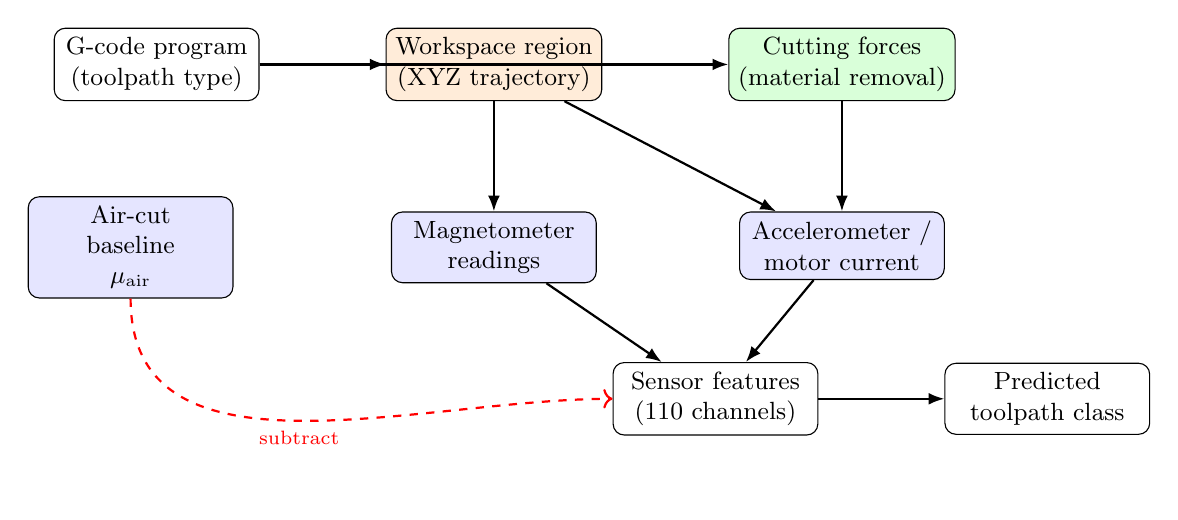
\begin{tikzpicture}[
    node distance=1.4cm and 1.6cm,
    every node/.style={font=\small},
    var/.style={rectangle, draw, rounded corners, minimum width=2.6cm, minimum height=0.8cm, align=center},
    obs/.style={var, fill=blue!10},
    confound/.style={var, fill=orange!15},
    process/.style={var, fill=green!15},
    arrow/.style={-{Latex[length=2mm]}, thick},
    intervene/.style={->, dashed, thick, red},
]
% Top row
\node[var] (gcode) {G-code program\\(toolpath type)};
\node[confound, right=of gcode] (workspace) {Workspace region\\(XYZ trajectory)};
\node[process, right=of workspace] (forces) {Cutting forces\\(material removal)};

% Middle row
\node[obs, below=of workspace] (mag) {Magnetometer\\readings};
\node[obs, below=of forces] (motion) {Accelerometer /\\motor current};

% Bottom row
\node[var, below right=1.0cm and 0.2cm of mag] (features) {Sensor features\\(110 channels)};
\node[var, right=of features] (label) {Predicted\\toolpath class};

% Air-cut reference (off to side)
\node[obs, left=2.0cm of mag] (air) {Air-cut\\baseline\\$\boldsymbol{\mu}_\text{air}$};

% Arrows
\draw[arrow] (gcode) -- (workspace);
\draw[arrow] (gcode) -- (forces);
\draw[arrow] (workspace) -- (mag);
\draw[arrow] (workspace) -- (motion);
\draw[arrow] (forces) -- (motion);
\draw[arrow] (mag) -- (features);
\draw[arrow] (motion) -- (features);
\draw[arrow] (features) -- (label);

% Air-cut intervention
\draw[intervene] (air) to[out=270, in=180] node[below, font=\scriptsize, sloped] {subtract} (features);
\end{tikzpicture}
\caption{Causal structure of the toolpath classification task. Solid arrows represent causal dependencies in the data-generating process. The G-code program is the root cause of both workspace region (a confound) and cutting forces (the process-relevant signal). Magnetometer features are downstream of workspace region only, making them position encoders. Accelerometer and motor-current features are downstream of both workspace region and cutting forces. The dashed red arrow represents the air-cut referencing intervention: subtracting the air-cut baseline from active features removes the workspace-dependent component, leaving the cutting-force component. Because the air-cut and active programs in our dataset traverse \emph{similar but not identical} workspace regions, this subtraction is partial (Section~\ref{sec:results}). Note that under the shallow-DOC UHMW-PE conditions of this study, the cutting-forces $\rightarrow$ motion-features arrow carries a small signal ($\sim$1--2~N at the tool); on metallic workpieces with realistic cutting forces (50--500~N), this arrow would be substantially stronger, shifting the relative balance of position-encoded versus force-encoded discrimination.}
\label{fig:causal_dag}
\end{figure}

This structural model explains four otherwise puzzling observations. First, magnetometer features dominate feature importance because they are directly downstream of the workspace-region confound, which carries nearly all the class signal. Second, removing magnetometer channels does not destroy classification accuracy because accelerometer and motor-current features are also downstream of workspace region (via trajectory-dependent acceleration patterns). Third, air-cut referencing helps even on confound-free features because it removes workspace-dependent components from the accelerometer and current channels as well, isolating their force-relevant residuals. Fourth, cross-condition transfer fails (37\% accuracy) because the air-cut and active-cut conditions used different G-code programs and thus produced different workspace regions, so the position-encoded features do not transfer; the small force-relevant signal would transfer but is dominated by the position component in the raw representation. Together these explain why the paper's headline result (100\% accuracy) is not the contribution. The contribution is identifying the causal structure that makes such results possible and providing a methodology for separating the position-encoded path from the force-relevant path.

\subsection{Limitations and Future Work}

\textbf{No independent test set.} Beyond the single internal held-out split (Section~\ref{sec:results}: 12 of the 51 runs, evaluated once), all evaluations rely on cross-validation (5-fold stratified, 20 repeats) on the same 51 active-cutting runs. That internal split shares the machine, session, and CAM programs of the training data, so it guards against fold-reuse leakage but is \emph{not} an independent test of generalization. With 100 CV evaluations, every sample also appears in many train/test splits. An \emph{independent} test set from a future collection round (a new session, and ideally a second machine) would provide stronger evidence of generalization. Within the existing data, the leave-$K$-runs-out analysis ($K \leq 3$) is the closest approximation.

\textbf{Single machine.} All data is collected from one Bantam Tools Explorer CNC mill. The central hypothesis, that air-cut referencing produces machine-independent fingerprints, cannot be fully validated without cross-machine experiments. The strong generalization results (leave-$K$-out accuracy) suggest robustness to within-machine variation but do not address between-machine variation.

\textbf{Different CAM programs.} The air-cut and active-cutting data used different CAM-generated G-code programs, preventing point-by-point signal subtraction. The temporal binning approach compensates for this, but future data collection should use identical G-code programs for both conditions to enable direct comparison.

\textbf{Limited toolpath diversity.} Three toolpath types with fixed cutting parameters (0.150'' stepover, 0.025'' depth) provide a clean classification task but do not test discrimination between subtle variations within a toolpath type.

\textbf{Workpiece material and cutting forces.} The UHMW-PE workpiece produces extremely low cutting forces ($\sim$1--2~N for a \SI{6.35}{\milli\meter} endmill at \SI{0.635}{\milli\meter} DOC) compared to metals. This means the ``process-specific signal'' isolated by air-cut referencing is dominated by trajectory differences and quasi-static motion dynamics rather than cutting force signatures. On metallic workpieces with higher cutting forces, the sensor signals would contain a larger cutting-force component, potentially making the accelerometer and current channels more discriminative relative to the magnetometer position proxy.

\textbf{Low sampling rate and decimation.} The \SI{4}{\hertz} effective sampling rate (decimated from \SI{119}{\hertz} IMU and \SI{1}{\kilo\hertz} DAQ without explicit anti-aliasing) captures only quasi-static machine motion, not cutting vibration. Higher-rate acquisition retaining the native DAQ bandwidth would enable frequency-domain features (e.g., power spectral density at cutting-relevant frequencies) that are unavailable in this study.

\textbf{Small dataset.} With 51 active-cutting runs and $\leq$19 runs per class, the dataset is adequate for the current three-class problem but may be insufficient for more complex tasks or deep learning approaches.

\textbf{Near-perfect accuracy.} The 100\% RF accuracy across all methods raises concerns about task difficulty. The three toolpath types are structurally quite different (continuous adaptive, back-and-forth facing, concentric pocketing), making them inherently easy to distinguish. Testing on more similar toolpath variants would better evaluate the methods' discriminative power.


\section{Conclusions}\label{sec:conclusion}

This paper introduced air-cut referencing with temporal binning as a methodology for extracting toolpath fingerprints from CNC sensor data. We evaluated four signal isolation methods across three classifiers for three-class toolpath classification (adaptive clearing, facing, pocketing) on a dataset of 51 active-cutting and 55 air-cutting runs from a desktop CNC mill.

The key findings are:

\begin{enumerate}
    \item \textbf{Task difficulty context.} Trivial baseline analysis reveals that the three toolpath types are separable from program metadata alone (G-code line range: 100\%, mean position: 98\%). This contextualizes the high sensor-based accuracy and underscores that the primary contribution is methodological rather than accuracy-driven.

    \item \textbf{Air-cut referencing provides genuine, confound-independent benefit.} When all position-confounded channels (magnetometers, color, pressure, proximity) are excluded (784 features), raw RF drops to 96.7\% with a minimum fold accuracy of 81.8\%, while the subtracted and ratio methods maintain \textbf{perfect 100\% accuracy across all 100 repeated CV evaluations} and z-score remains near-perfect (99.0\%, minimum 90\%). This demonstrates that the referencing benefit is not an artifact of the magnetometer position-encoding confound. The Friedman test ($p < 10^{-6}$) confirms statistical significance, and noise robustness analysis shows referenced features maintain accuracy up to $1.0\times$ noise.

    \item \textbf{Process dynamics are recoverable once position is controlled.} On a damaged-tool detection task using the same G-code programs (so workspace position is held constant), Random Forest reaches 98.5\% accuracy (balanced 0.99, damage-class $F_1 = 0.97$), with discriminative importance shifting from the magnetometer (0.1\%) to the accelerometer and acoustic-RMS channels (74\% combined). This is the most process-relevant result and a direct tool-condition-monitoring application; air-cut referencing is neutral here, consistent with the causal model (referencing helps only when a position confound is present).

    \item \textbf{Temporal structure is informative.} Temporal binning (20 bins) outperforms whole-run summary statistics (100\% vs.\ 98\%), and produces interpretable fingerprint visualizations that reveal toolpath-specific sensor dynamics.

    \item \textbf{Minimal sensor requirements.} A single bed-mounted IMU achieves 100\% accuracy with 238 features. Only 5 training runs per class suffice for 96.4\% accuracy.

    \item \textbf{Competitive with modern methods.} ROCKET-style random convolutional features achieve comparable accuracy (98--100\%), confirming the task's accessibility while validating that our interpretable approach does not sacrifice performance.
\end{enumerate}

A notable limitation is that the air-cut and active-cutting data used different CAM-generated G-code programs, preventing direct G-code-aligned signal subtraction. The temporal binning approach compensates for this, but future data collection should use identical programs.

Future work will focus on: (1)~within-toolpath-type parameter discrimination (e.g., different stepovers), where trivial baselines cannot help and air-cut referencing should provide greater benefit; (2)~cross-machine validation to test transferability of referenced fingerprints; and (3)~higher-rate data acquisition to enable frequency-domain features.


\vspace{6pt}

\authorcontributions{Conceptualization, S.S.E. and R.S.P.; methodology, S.S.E.; software, S.S.E.; validation, S.S.E.; formal analysis, S.S.E.; investigation, S.S.E.; resources, M.S.S.; data curation, S.S.E. and R.S.P.; writing---original draft, S.S.E.; writing---review \& editing, R.S.P. and M.S.S.; visualization, S.S.E.; supervision, R.S.P. and M.S.S.; project administration, R.S.P. All authors have read and agreed to the published version of the manuscript.}

\funding{This material is based upon work partially supported by the Office of Naval Research (ONR) under Contract no. N000142412129.}

\acknowledgments{This material is based upon work partially supported by the Office of Naval Research (ONR) under Contract no. N000142412129. Any opinions, findings, and conclusions or recommendations expressed in this material are those of the author(s) and do not necessarily reflect the view of the ONR. The authors thank the Department of Industrial Systems Engineering at the University of Rhode Island for providing laboratory facilities and computational resources.}

\conflictsofinterest{The authors declare no conflict of interest.}

\newcommand{\dataavailabilitytext}{The sensor datasets and analysis code generated during this study are publicly available at \url{https://github.com/stephenseacuello/gcode_fingerprinting}.}
\ifdefined\dataavailability
  \dataavailability{\dataavailabilitytext}
\else
  \noindent\textbf{Data Availability Statement:} \dataavailabilitytext
\fi

\bibliography{references}

\end{document}
